\documentclass[lineno]{JFM-FLM_Au}

\usepackage{xcolor}
\usepackage{tikz}
\usetikzlibrary{calc,arrows.meta}
\usepackage{xcolor}  % if not already loaded
\newcommand{\tbd}[1]{\textcolor{red}{\ensuremath{\langle\mbox{\small #1}\rangle}}}
\definecolor{jfmblue}{RGB}{0,56,168}

\hypersetup{
  colorlinks=true,
  citecolor=blue,
  linkcolor=jfmblue,
  urlcolor=jfmblue
}

\newtheorem{lemma}{Lemma}
\newtheorem{corollary}{Corollary}

\lefttitle{Author 1 et al.}
\righttitle{Journal of Fluid Mechanics}

\title{Turbulence distortion and the pre-impact spectral tensor in airfoil leading-edge noise}

\author{Author 1\aff{1}, Author 2\aff{1} \and Author 3\aff{2}}

\affiliation{\aff{1}Department, Institution, City, Country
\aff{2}Department, Institution, City, Country}

\corresau{Author 1, email}

\begin{document}
\maketitle

\begin{abstract}
This file contains information for authors planning to submit a paper to the {\it Journal of Fluid Mechanics}. The document was generated in {\LaTeX} using the JFM class file and supporting files provided on the JFM website \href{https://www.cambridge.org/core/journals/journal-of-fluid-mechanics/information/author-instructions/preparing-your-materials}{here}, and the source files can be used as a template for submissions (please note that this is mandatory for {\it JFM Rapids}). Full author instructions can be found on the \href{https://www.cambridge.org/core/journals/journal-of-fluid-mechanics/information/author-instructions}{JFM website}. The present paragraph appears in the \verb}abstract} environment. All papers should feature a single-paragraph abstract of no more than 250 words which must not spill onto the second page of the manuscript.
\end{abstract}

\begin{keywords}
Authors should not enter keywords on the manuscript, as these must be chosen by the author during the online submission process and will then be added during the typesetting process (see \href{https://www.cambridge.org/core/services/aop-file-manager/file/61436b61ff7f3cfab749ce3a/JFM-Keywords-Sept-2021.pdf.}{Keyword PDF} for the full list).  Other classifications will be added at the same time.
\end{keywords}

%{\bf MSC Codes }  {\it(Optional)} Please enter your MSC Codes here

% =========================================================================
% Introduction — Turbulence distortion and the pre-impact spectral tensor
% in airfoil leading-edge noise
% Target journal: Journal of Fluid Mechanics (natbib, \citep / \citet)
% =========================================================================

\section{Introduction}
\label{sec:introduction}

The interaction of free-stream turbulence with the leading edge of a lifting
surface is among the dominant broadband noise mechanisms in low-Mach-number
aeroacoustics, governing the acoustic signature of fans, propellers,
turbomachinery stages operating in wakes or distorted inflow, and wind
turbines in the atmospheric boundary layer
\citep{Amiet1975,PatersonAmiet1976,Moriarty2005,DevenportStaubsGlegg2010}.
As trailing-edge and tonal sources have been progressively attenuated through
geometric optimisation and flow control, turbulence-interaction noise has
become an increasingly binding constraint on low-noise design, and the demand
for predictive — rather than calibrated — models of this source has grown
correspondingly \citep{KimHaeriJoseph2016,SharmaSarradjSchmidt2020,SharmaHerr2024}.

The classical description of the generation mechanism is well established.
An incoming vortical disturbance, decomposed into sinusoidal gusts, induces
an unsteady loading on the airfoil whose linear transfer function was first
derived for incompressible flow by \citet{Sears1941} and generalised to
oblique gusts and subsonic compressible flow by \citet{Graham1970}. The
unsteady surface pressure radiates to the far field by a scattering process
whose theoretical foundations lie in the acoustic analogy of
\citet{Lighthill1952}, its extension to flows containing stationary and
moving surfaces \citep{Curle1955,FfowcsWilliamsHawkings1969}, and the
analysis of scattering by sharp edges \citep{FfowcsWilliamsHall1970}; unified
treatments are given by \citet{Goldstein1976} and, in the vortex-sound
framework, by \citet{Howe2003}. Building on these elements,
\citet{Amiet1975} formulated the canonical leading-edge noise model: the
far-field pressure spectral density is expressed as the product of an
aerodynamic--acoustic transfer function, derived for a semi-infinite flat
plate, and the wavenumber spectrum of the incident velocity fluctuations.
The accompanying experiments of \citet{PatersonAmiet1976} established the
quantitative credibility of this formulation, and subsequent analytical
extensions have refined the finite-chord and back-scattering corrections
while retaining its overall architecture
\citep{RogerMoreau2005,MoreauRoger2009}.

The predictive power of this architecture rests on a specific set of
assumptions about the incident turbulence. The incoming field is taken to be
frozen in the sense of \citet{Taylor1938}, convecting toward the leading edge
at the free-stream velocity without modification by the mean flow; it is
usually modelled as homogeneous and isotropic, so that the full spectral
tensor is parametrised by an intensity and an integral length scale; and, of
the nine tensor components, only the wall-normal (upwash) velocity spectrum
enters the prediction, since for a flat plate at zero incidence only the
upwash produces unsteady loading \citep{Amiet1975,Goldstein1976}. Under
these assumptions the turbulence appears in the model purely as a prescribed
boundary datum: the entire physics of the interaction is delegated to the
acoustic transfer function, and the spectrum evaluated far upstream is
implicitly identified with the spectrum that forces the leading edge.

A substantial body of experimental and computational work has tested this
framework and delineated where it fails. \citet{PatersonAmiet1976} already
noted an overprediction of high-frequency noise for airfoils of finite
thickness, a trend confirmed systematically by \citet{OlsenWagner1982} and
quantified in later studies as a thickness- and frequency-dependent
attenuation relative to the flat-plate result
\citep{Gershfeld2004,Lysak2013,Gill2013}. Measurements of unsteady surface
pressure beneath grid turbulence showed that mean loading and geometry
modify the pressure response in ways not captured by thin-airfoil theory
\citep{MishDevenport2006}, and acoustic measurements on families of real
airfoils demonstrated that the high-frequency noise reduction is not
controlled by a single geometric parameter such as the leading-edge radius or
maximum thickness \citep{DevenportStaubsGlegg2010,Hall2011}. On the
computational side, gust--airfoil interaction in realistic mean flows
\citep{LockardMorris1998}, high-fidelity simulations of
aerofoil--turbulence interaction \citep{KimHaeriJoseph2016}, and, more
recently, lattice Boltzmann simulations of grid-generated turbulence
impinging on a NACA\,0012 airfoil
\citep{Trascinelli2023,Piccolo2024} have resolved both the hydrodynamic
near field and the acoustic radiation, while dedicated aeroacoustic
facilities have characterised the inflow turbulence with increasing care
\citep{Bowen2022}. These studies agree that finite-thickness effects are
real, scale-dependent and acoustically significant.

What they leave less settled is where in the causal chain those effects
should be attributed. Most corrections developed to reconcile flat-plate
theory with thick-airfoil data act at the level of the acoustic response:
streamline-based modifications of the incident gust along the mean-flow
trajectory \citep{Guidati1997,Moriarty2005}, exponential high-frequency
attenuation factors \citep{Gershfeld2004,Lysak2013}, or panel-method
generalisations of the transfer function to realistic geometries
\citep{GleggDevenport2010Panel}. Each of these improves agreement within its
calibration range, but each also absorbs the underlying physics — the
modification of the turbulence itself before it reaches the surface — into
an effective acoustic operator. The causal chain implied by the flow is
longer than the one represented in the models: the upstream turbulence
tensor is first transformed by the decelerating, straining flow ahead of the
stagnation region, and only the resulting pre-impact state is available to
force the unsteady loading. Classical leading-edge noise theories describe
the scattering and acoustic response once an incoming gust or spectrum has
been specified; comparatively little attention has been given to the
transformation that converts the measured upstream turbulence into the
effective state experienced by the leading edge.

The physical and mathematical language appropriate to this earlier stage
exists, and is that of rapid distortion theory (RDT). Following the analysis
of a single Fourier mode under uniform straining by \citet{Taylor1935},
\citet{BatchelorProudman1954} derived the linear response of homogeneous
turbulence to rapid mean deformation, and \citet{Hunt1973} extended the
theory to flow around two-dimensional bluff bodies, identifying the distinct
roles of mean-strain distortion, inviscid blocking by the surface, and the
concentration of vorticity near the stagnation streamline; the blocking
mechanism near a plane boundary was analysed separately by
\citet{HuntGraham1978}. Hot-wire measurements upstream of bluff bodies
confirmed the predicted behaviour, with large-scale wall-normal fluctuations
suppressed by blocking and smaller scales amplified by straining, the
crossover being set by the ratio of eddy size to body dimension
\citep{Bearman1972,BritterHuntMumford1979}. In the aeroacoustic context,
\citet{GoldsteinAtassi1976} showed that the unsteady airfoil response is
fundamentally altered when the distortion of the incident gust by the steady
potential flow is retained, and \citet{Goldstein1978} generalised the
splitting of the disturbance field to arbitrary obstacles;
\citet{HuntCarruthers1990} review the scope and limitations of the linear
theory. These results establish that the quantity transformed by the
leading-edge flow is not a scalar intensity but the full spectral tensor:
the deformation acts differently on different components and different
wavenumbers, generating anisotropy that is naturally described by the
Reynolds-stress anisotropy invariants of \citet{LumleyNewman1977}, and
modified further by pressure--strain redistribution beyond the reach of
linear theory \citep{SpezialeSarkarGatski1991,Pope2000}. Recent work has
begun to import these ideas into noise prediction: RDT-corrected upwash
spectra improve Amiet-type predictions for thick airfoils
\citep{deSantana2016,dosSantos2023}, distortion has been invoked to explain
the noise reduction of porous leading edges \citep{Zamponi2020}, and
combined experimental--numerical studies have measured the one-dimensional
spectral modification directly in the stagnation region \citep{Piccolo2024}.

Taken together, however, the literature characterises this pre-impact
transformation only in reduced form — as a correction to a single velocity
spectrum, a streamline-integrated velocity ratio, or a fitted attenuation
function. Several questions of principle remain open. It has not been
established empirically whether the mapping from the upstream spectral
tensor $\Phi^{\infty}_{ij}$ to the pre-impact tensor $\Phi^{\mathrm{LE}}_{ij}$
can be represented by a scalar, frequency-dependent gain, or whether it is
irreducibly tensorial, coupling components and redistributing energy
anisotropically. The scale dependence of the mapping — in particular,
whether the leading-edge radius $r_{\mathrm{LE}}$ acts as the geometric
filter separating strongly and weakly distorted scales through the
dimensionless wavenumber $\kappa = k\,r_{\mathrm{LE}}$ — has been inferred
from acoustic far-field trends \citep{Gill2013,DevenportStaubsGlegg2010} but
not measured directly on the turbulence field surrounding the leading edge.
Nor is it known to what extent the transformation departs from linear RDT,
through pressure--strain redistribution and finite-time nonlinear effects,
in the regime of practical interest. Until these questions are answered,
the common practice of inserting an upstream-measured spectrum directly into
a leading-edge noise model rests on an assumption whose error is neither
quantified nor even of known sign across frequency.

The present paper addresses these questions by isolating the pre-impact
transformation itself as the object of study. We perform wall-modelled
large-eddy simulations, using a lattice Boltzmann method, of grid-generated
turbulence convecting onto a NACA\,0012 airfoil at chord-based Reynolds
number $Re_c \approx 5.1\times10^{5}$ and free-stream Mach number
$M = 0.059$, and we compare the turbulence state on planar reference patches
upstream of the airfoil with that on a toroidal sampling surface enclosing
the leading edge. The comparison is organised around the hypothesis of a
distortion mapping,
$\Phi^{\mathrm{LE}}_{ij}(\boldsymbol{k},\omega)
 = \mathcal{D}_{ijmn}(\boldsymbol{k},\theta)\,
   \Phi^{\infty}_{mn}(\boldsymbol{k},\omega)$,
in which a fourth-order, scale- and orientation-dependent operator
$\mathcal{D}$, structurally motivated by rapid distortion theory, relates
the two spectral tensors. We emphasise that $\mathcal{D}$ is introduced
here as a diagnostic and organising framework rather than as an established
closed-form model: the simulations provide its diagonal and azimuthally
projected components through component-wise spectral gains $G_q(f)$ and
local-frame distortion maps, together with Reynolds-stress budgets and
Lumley-invariant trajectories that constrain its tensorial structure. A
preliminary account of this approach was given in
\citet{Sharma2026}. The results demonstrate that the transformation is
scale-dependent, with the transition between strong and weak distortion
organised by $\kappa = k\,r_{\mathrm{LE}}$; that it is component-dependent
and therefore not reducible to a scalar correction; and that the invariant
trajectories exhibit a transient eigenvalue reordering inconsistent with
purely linear distortion, implicating pressure--strain redistribution in the
pre-impact dynamics.

The remainder of the paper is organised as follows.
Section~\ref{sec:framework} develops the mathematical framework that casts
turbulence distortion as an operator mapping between spectral tensors and
identifies $\kappa$ and the integrated-strain parameter $\theta$ as the
governing dimensionless groups. Sections~\ref{sec:method}
and~\ref{sec:setup} describe the lattice Boltzmann solver, the subgrid-scale
and wall modelling, and the computational configuration, including the
turbulence-generating grid and the two-surface sampling strategy.
Sections~\ref{sec:flowfield}--\ref{sec:invariants} characterise the
evolution of the mean flow, Reynolds stresses and anisotropy invariants
between the upstream reference and the leading edge.
Section~\ref{sec:spectra} presents the patch-based spectral comparison, the
spectral gains $G_q(f)$ and the local-frame distortion maps that constitute
the empirical characterisation of $\mathcal{D}$. Section~\ref{sec:conclusions}
summarises the findings and discusses their implications for the structure
of predictive leading-edge noise models.

% Standalone-insertable figure for the JFM manuscript.
% Requires in preamble: \usepackage{tikz,graphicx,amsmath}
%                       \usetikzlibrary{calc,arrows.meta}
% (all already present in your new-aiaa preamble)

% \begin{figure}
% \centering
% \begin{tikzpicture}[>=Latex, font=\small]
%   % ---- mean flow ----
%   \foreach \y in {-1.3,-0.65,0.65,1.3}
%     \draw[->,gray] (-5.0,\y) -- (-4.3,\y);
%   \node[gray] at (-4.70,1.98) {$U_\infty\boldsymbol{e}_x$};
%   % ---- upstream reference plane ----
%   \draw[dashed,thick] (-3.6,-1.9) -- (-3.6,2.1);
%   \node at (-3.6,2.40) {$\mathcal{S}_\infty:\;\Phi^{\infty}_{ij}$};
%   % ---- airfoil: nose circle r_LE = 0.85 centred at origin, tail (6.5,0) --
%   \draw[thick,fill=gray!12]
%     (0,0.85) .. controls (2.3,0.60) and (5.0,0.20) .. (6.5,0)
%              .. controls (5.0,-0.20) and (2.3,-0.60) .. (0,-0.85)
%     arc (-90:-270:0.85);
%   \draw[densely dotted] (0,0) circle (0.85);    % osculating nose circle
%   \node[circle,fill,inner sep=0.7pt] at (0,0) {};
%   \draw[->] (0,0) -- (35:0.85);
%   \node at (1.12,0.55) {$r_{\mathrm{LE}}$};
%   % ---- pre-impact surface (conformal, offset delta_n) ----
%   \draw[dashed,thick] (95:1.30) arc (95:265:1.30);
%   \draw[gray!70] (243:1.30) -- (-1.45,-1.55);
%   \node[anchor=east] at (-1.40,-1.62) {$\mathcal{S}_{\mathrm{LE}}:\;\Phi^{\mathrm{LE}}_{ij}$};
%   \draw[<->] (-0.88,-0.16) -- (-1.27,-0.16);
%   \node[below] at (-1.07,-0.20) {$\delta_n$};
%   % ---- stagnation line, azimuth ----
%   \draw[gray] (-3.6,0) -- (-1.35,0);
%   \node[gray,below] at (-2.55,0) {$\theta=0$};
%   \draw[->] (-1.58,0) arc (180:123:1.58);
%   \node at (-1.78,0.72) {$\theta$};
%   % ---- local frame at drawing angle 120 deg (theta = 60 deg) ----
%   \coordinate (P) at (120:1.30);
%   \node[circle,fill,inner sep=0.7pt] at (P) {};
%   \draw[->,thick] (P) -- ++(120:0.60);
%   \node[anchor=south,inner sep=2pt] at ($(P)+(120:0.60)$)
%         {$\boldsymbol{e}_r=\boldsymbol{e}_n$};
%   \draw[->,thick] (P) -- ++(30:0.60);
%   \node[anchor=west,inner sep=2pt] at ($(P)+(30:0.60)$)
%         {$\boldsymbol{e}_\theta=\boldsymbol{e}_t$};
%   % ---- eddy glyphs: sphere -> tangentially elongated ellipse ----
%   \draw[gray!70] (-3.0,0.85) .. controls (-2.3,0.90) and (-1.9,1.05) .. (-1.55,1.35);
%   \draw (-3.0,0.85) circle (0.20);
%   \draw[rotate around={38:(-1.55,1.35)}] (-1.55,1.35) ellipse (0.33 and 0.11);
%   \node[align=center] at (-2.98,1.60)
%         {\footnotesize tangential extension,\\[-3pt]\footnotesize normal compression};
%   % ---- dimensions / plane note ----
%   \draw[<->] (-3.6,-1.95) -- (-0.85,-1.95);
%   \node[below] at (-2.22,-1.95) {$\ell_\infty$};
%   \node[align=left] at (4.7,1.55)
%         {\footnotesize midspan $(x,y)$ plane;\\[-2pt]
%          \footnotesize $\boldsymbol{e}_z$ out of plane};
% \end{tikzpicture}
% \caption{Configuration and definitions of \S\,\ref{sec:framework_states}.
% Turbulence carried by the uniform stream is characterised on the upstream
% reference plane $\mathcal{S}_\infty$ (a distance $\ell_\infty$ ahead of the
% leading edge) and again on the conformal pre-impact surface
% $\mathcal{S}_{\mathrm{LE}}$, offset $\delta_n \ll r_{\mathrm{LE}}$ from the
% nose. The azimuth $\theta$ is measured from the upstream stagnation line
% about the centre of the osculating nose circle (dotted); on that circle
% the cylindrical and surface-aligned frames coincide,
% $\boldsymbol{e}_r = \boldsymbol{e}_n$,
% $\boldsymbol{e}_\theta = \boldsymbol{e}_t$. The eddy glyphs indicate the
% sense of the strain (\ref{eq:strain_local}): tangential extension, normal
% compression.}
% \label{fig:framework_config}
% \end{figure}

% Standalone-insertable figure for the JFM manuscript.
% Requires in preamble: \usepackage{tikz,graphicx,amsmath}
%                       \usetikzlibrary{calc,arrows.meta}
% (all already present in your new-aiaa preamble)



% Standalone-insertable figure for the JFM manuscript.
% Requires in preamble: \usepackage{tikz,graphicx,amsmath}
%                       \usetikzlibrary{calc,arrows.meta}
% (all already present in your new-aiaa preamble)

% =========================================================================
% Section 2 (EXPANDED VERSION) — Theoretical framework: pre-impact
% distortion as a tensorial mapping.
% Target: Journal of Fluid Mechanics (natbib, \citep / \citet).
%
% NOTATION (must propagate through the manuscript):
%   \vartheta : integrated-strain (distortion) parameter  [was θ in conf. §II]
%   \theta    : azimuthal coordinate around the leading edge, in the
%               MIDSPAN (x,y) plane, θ = 0 on the upstream stagnation line.
%   Local cylindrical projection acts on (u,v) in the midspan plane, w
%   unchanged (published-PDF convention). >>> DECISION POINT: if the
%   post-processing projected (v,w) in the (y,z) plane instead, §2.6 and
%   eq. (trace) must be changed to match. <<<
%
% All citations resolve to entries in references.bib +
% references_framework_additions.bib (all verified). No new references.
% =========================================================================

\section{Theoretical framework: pre-impact distortion as a tensorial mapping}
\label{sec:framework}

\subsection{Flow configuration, governing equations, and the two turbulence
states}
\label{sec:framework_states}

We consider statistically stationary turbulence, generated far upstream and
carried by a uniform mean stream $U_\infty\boldsymbol{e}_x$, convecting onto
a symmetric airfoil of chord $c$ and leading-edge radius $r_{\mathrm{LE}}$
at zero incidence. Cartesian coordinates $(x,y,z)$ denote the streamwise,
transverse and spanwise directions; the leading edge lies at
$x = x_{\mathrm{LE}}$, $y = 0$. The statistics are homogeneous in $z$ and
stationary in $t$, and the turbulence is weak,
$\epsilon \equiv u'_\infty/U_\infty \ll 1$, where $u'_\infty$ is the
upstream root-mean-square velocity fluctuation. The velocity and pressure
are decomposed as
$\boldsymbol{u} = \overline{\boldsymbol{U}}(\boldsymbol{x})
+ \boldsymbol{u}'(\boldsymbol{x},t)$,
$p = \overline{P}(\boldsymbol{x}) + p'(\boldsymbol{x},t)$, and at leading
order in $\epsilon$ the mean flow is the steady flow past the airfoil,
unmodified by the fluctuations. Outside the thin attached boundary layer
the mean flow in the nose region may be treated as irrotational; this is a
modelling assumption whose principal consequence --- the absence of mean
vorticity in the fluctuation dynamics below --- simplifies the linear
theory without altering its structure.

Substituting the decomposition into the Navier--Stokes equations and
retaining terms of first order in the fluctuations gives the linearised
disturbance equation
\begin{equation}
  \frac{\mathrm{D}u_i'}{\mathrm{D}t}
  + u_j'\,\frac{\partial \overline{U}_i}{\partial x_j}
  = -\frac{1}{\rho}\frac{\partial p'}{\partial x_i}
  + \nu\nabla^2 u_i',
  \qquad
  \frac{\mathrm{D}}{\mathrm{D}t}
  \equiv \frac{\partial}{\partial t}
  + \overline{U}_j\frac{\partial}{\partial x_j},
  \label{eq:linearised}
\end{equation}
together with $\nabla\cdot\boldsymbol{u}' = 0$. The neglected nonlinear
term is smaller than the retained mean-gradient term by the ratio of the
mean strain rate to the eddy turnover rate; the regime in which
(\ref{eq:linearised}) governs the transformation --- rapid distortion ---
is quantified in \S\,\ref{sec:framework_hypothesis}
\citep{BatchelorProudman1954,HuntCarruthers1990}. Taking the curl of
(\ref{eq:linearised}) for an irrotational mean flow and neglecting
viscosity at the energy-containing scales yields
\begin{equation}
  \frac{\mathrm{D}\omega_i'}{\mathrm{D}t}
  = \omega_j'\,\frac{\partial \overline{U}_i}{\partial x_j},
  \label{eq:vorticity_lin}
\end{equation}
i.e. the fluctuating vorticity is rearranged and reoriented by the mean
velocity gradient exactly as a material line element, with the classical
Cauchy solution
\begin{equation}
  \omega_i'(\boldsymbol{x},t)
  = F_{ij}\,\omega_j'(\boldsymbol{X},0),
  \qquad
  F_{ij} = \frac{\partial x_i}{\partial X_j},
  \label{eq:cauchy}
\end{equation}
where $\mathsf{F}$ is the deformation-gradient tensor of the mean flow
along the trajectory carrying the material point from $\boldsymbol{X}$ to
$\boldsymbol{x}$ \citep{BatchelorProudman1954,HuntCarruthers1990}.
Equations (\ref{eq:vorticity_lin})--(\ref{eq:cauchy}) are the dynamical
core of everything that follows: the mean flow acts on the turbulence
through $\mathsf{F}$, and the pressure acts only to maintain
incompressibility.

The analysis is organised around two turbulence states, defined as
statistical ensembles on control surfaces rather than by reference to a
measurement apparatus. The \emph{upstream state} is the ensemble of
fluctuations on a plane $\mathcal{S}_\infty$ normal to
$\boldsymbol{e}_x$, a distance $\ell_\infty$ ahead of the leading edge,
with $\ell_\infty$ large enough that the mean flow on $\mathcal{S}_\infty$
is uniform to within a prescribed tolerance, yet small enough that free
decay between $\mathcal{S}_\infty$ and the airfoil is negligible compared
with the distortion to be quantified. The \emph{pre-impact state} is the
ensemble on a surface $\mathcal{S}_{\mathrm{LE}}$ conformal to the nose,
displaced from the wall by a fixed offset $\delta_n \ll r_{\mathrm{LE}}$,
on which the fluctuations have traversed the stagnation-region strain but
have not yet participated in the scattering that generates the acoustic
field. The acoustic response is outside the present framework: we
characterise the transformation between $\mathcal{S}_\infty$ and
$\mathcal{S}_{\mathrm{LE}}$ that precedes and conditions the scattering
problem of classical theory \citep{Amiet1975,Goldstein1976}.

Two local frames are attached to $\mathcal{S}_{\mathrm{LE}}$. Because the
nose is locally cylindrical, points on $\mathcal{S}_{\mathrm{LE}}$ in the
midspan plane are parametrised by the azimuth $\theta$ about the centre of
the osculating nose circle, with $\theta = 0$ on the upstream stagnation
line; the associated unit vectors $\boldsymbol{e}_r(\theta)$,
$\boldsymbol{e}_\theta(\theta)$ lie in the $(x,y)$ plane and complete a
right-handed triad with $\boldsymbol{e}_z$. On the nose circle the
surface-aligned frame $(t,n,z)$ coincides with the cylindrical frame,
$\boldsymbol{e}_n = \boldsymbol{e}_r$,
$\boldsymbol{e}_t = \boldsymbol{e}_\theta$, so that `wall-normal' and
`radial' may be used interchangeably there; away from the nose circle the
frames separate and the distinction is retained. The configuration, the two control surfaces and the local frames are
summarised in figure~\ref{fig:framework_config}.
\begin{figure}
\centering
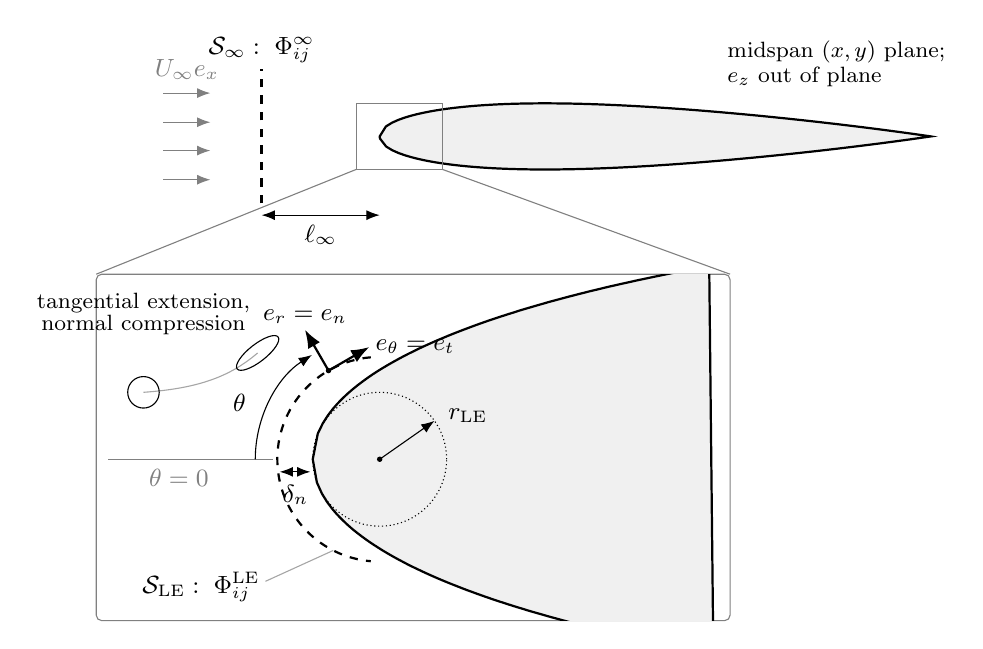
\begin{tikzpicture}[>=Latex, font=\small]
% ===================== GLOBAL VIEW (true NACA 0012, chord 7) ============
\begin{scope}[shift={(0,4.1)}]
  % mean flow
  \foreach \y in {-0.55,-0.18,0.18,0.55}
    \draw[->,gray] (-2.75,\y) -- (-2.15,\y);
  \node[gray] at (-2.45,0.85) {$U_\infty\boldsymbol{e}_x$};
  % upstream reference plane
  \draw[dashed,thick] (-1.5,-0.85) -- (-1.5,0.85);
  \node at (-1.5,1.10) {$\mathcal{S}_\infty:\;\Phi^{\infty}_{ij}$};
  \draw[<->] (-1.5,-1.00) -- (0,-1.00);
  \node[below] at (-0.75,-1.00) {$\ell_\infty$};
  % true NACA 0012, chord c = 7, y = 0.6c*(0.2969 sqrt(x) - 0.1260x
  %   - 0.3516x^2 + 0.2843x^3 - 0.1036x^4), closed trailing edge
  \draw[thick,fill=gray!12]
    plot[domain=0:1,samples=90]
      ({7*\x},{4.2*(0.2969*sqrt(\x)-0.1260*\x-0.3516*\x*\x
               +0.2843*\x*\x*\x-0.1036*\x*\x*\x*\x)})
    -- plot[domain=1:0,samples=90]
      ({7*\x},{-4.2*(0.2969*sqrt(\x)-0.1260*\x-0.3516*\x*\x
               +0.2843*\x*\x*\x-0.1036*\x*\x*\x*\x)})
    -- cycle;
  \node[align=left] at (5.8,0.92)
        {\footnotesize midspan $(x,y)$ plane;\\[-2pt]
         \footnotesize $\boldsymbol{e}_z$ out of plane};
  % zoom box around the nose
  \draw[gray] (-0.30,-0.42) rectangle (0.80,0.42);
\end{scope}
% ---- zoom connection lines ----
\draw[gray,thin] (-0.30,3.68) -- (-3.60,2.35);
\draw[gray,thin] (0.80,3.68) -- (4.45,2.35);
% ===================== MAGNIFIED NOSE REGION ============================
% Osculating-circle centre at local origin; LE (stagnation point) at
% (-0.85,0); magnification such that r_LE = 0.0158c -> 0.85 drawing units,
% i.e. chord = 53.55 units; same NACA 0012 polynomial, x/c in [0,0.095].
\draw[gray,rounded corners=2pt] (-3.60,-2.05) rectangle (4.45,2.35);
\begin{scope}
  \clip (-3.60,-2.05) rectangle (4.45,2.35);
  \draw[thick,fill=gray!12]
    plot[domain=0:0.095,samples=80]
      ({53.55*\x-0.85},{32.13*(0.2969*sqrt(\x)-0.1260*\x-0.3516*\x*\x
               +0.2843*\x*\x*\x-0.1036*\x*\x*\x*\x)})
    -- plot[domain=0.095:0,samples=80]
      ({53.55*\x-0.85},{-32.13*(0.2969*sqrt(\x)-0.1260*\x-0.3516*\x*\x
               +0.2843*\x*\x*\x-0.1036*\x*\x*\x*\x)})
    -- cycle;
\end{scope}
% osculating nose circle, r_LE
\draw[densely dotted] (0,0) circle (0.85);
\node[circle,fill,inner sep=0.7pt] at (0,0) {};
\draw[->] (0,0) -- (35:0.85);
\node at (1.12,0.55) {$r_{\mathrm{LE}}$};
% pre-impact surface (conformal, offset delta_n)
\draw[dashed,thick] (95:1.30) arc (95:265:1.30);
\draw[gray!70] (243:1.30) -- (-1.45,-1.55);
\node[anchor=east] at (-1.40,-1.62) {$\mathcal{S}_{\mathrm{LE}}:\;\Phi^{\mathrm{LE}}_{ij}$};
\draw[<->] (-0.88,-0.16) -- (-1.27,-0.16);
\node[below] at (-1.07,-0.20) {$\delta_n$};
% stagnation line, azimuth
\draw[gray] (-3.45,0) -- (-1.35,0);
\node[gray,below] at (-2.55,0) {$\theta=0$};
\draw[->] (-1.58,0) arc (180:123:1.58);
\node at (-1.78,0.72) {$\theta$};
% local frame at drawing angle 120 deg (theta = 60 deg)
\coordinate (P) at (120:1.30);
\node[circle,fill,inner sep=0.7pt] at (P) {};
\draw[->,thick] (P) -- ++(120:0.60);
\node[anchor=south,inner sep=2pt] at ($(P)+(120:0.60)$)
      {$\boldsymbol{e}_r=\boldsymbol{e}_n$};
\draw[->,thick] (P) -- ++(30:0.60);
\node[anchor=west,inner sep=2pt] at ($(P)+(30:0.60)$)
      {$\boldsymbol{e}_\theta=\boldsymbol{e}_t$};
% eddy glyphs: sphere -> tangentially elongated ellipse
\draw[gray!70] (-3.0,0.85) .. controls (-2.3,0.90) and (-1.9,1.05) .. (-1.55,1.35);
\draw (-3.0,0.85) circle (0.20);
\draw[rotate around={38:(-1.55,1.35)}] (-1.55,1.35) ellipse (0.33 and 0.11);
\node[align=center] at (-3.,1.85)
      {\footnotesize tangential extension,\\[-3pt]\footnotesize normal compression};
\end{tikzpicture}
\caption{Configuration and definitions of \S\,\ref{sec:framework_states}.
Top: turbulence carried by the uniform stream is characterised on the
upstream reference plane $\mathcal{S}_\infty$, a distance $\ell_\infty$
ahead of an airfoil at zero incidence (true profile). Bottom:
magnified nose region. The pre-impact state is sampled on the conformal
surface $\mathcal{S}_{\mathrm{LE}}$, offset
$\delta_n \ll r_{\mathrm{LE}}$ from the nose; the azimuth $\theta$ is
measured from the upstream stagnation line about the centre of the
osculating nose circle (dotted), on which the cylindrical and
surface-aligned frames coincide, $\boldsymbol{e}_r = \boldsymbol{e}_n$,
$\boldsymbol{e}_\theta = \boldsymbol{e}_t$. The eddy glyphs indicate the
sense of the strain (\ref{eq:strain_local}): tangential extension, normal
compression.}
\label{fig:framework_config}
\end{figure}
Near the surface around the nose, the mean rate of strain takes the
approximate plane form
\begin{equation}
  \mathsf{S} \;\approx\;
  a\,(\boldsymbol{e}_t\boldsymbol{e}_t - \boldsymbol{e}_n\boldsymbol{e}_n),
  \qquad a > 0,
  \label{eq:strain_local}
\end{equation}
i.e. extension along the surface tangent, compression along the surface
normal, spanwise neutral. We emphasise that (\ref{eq:strain_local}) is
written in the local surface frame: on the upstream stagnation streamline,
where $\boldsymbol{e}_n = -\boldsymbol{e}_x$, the same tensor describes
streamwise \emph{compression}
($\partial\overline{U}/\partial x < 0$ as the flow decelerates toward the
stagnation point) and transverse extension. For the idealised uniform plane
strain (\ref{eq:strain_local}) sustained over a time $\tau$, the
deformation gradient in the $(t,n,z)$ triad is exactly
\begin{equation}
  \mathsf{F}(\vartheta)
  = \mathrm{diag}\!\left(\mathrm{e}^{\vartheta},\,
                          \mathrm{e}^{-\vartheta},\, 1\right),
  \qquad
  \vartheta = a\tau,
  \label{eq:Fdiag}
\end{equation}
which preserves volume, $\det\mathsf{F} = 1$, as required by
incompressibility of the mean flow. This is the canonical configuration of
rapid distortion theory \citep{BatchelorProudman1954,Hunt1973}, and the
dimensionless accumulated strain $\vartheta$ introduced in
(\ref{eq:Fdiag}) --- generalised to non-uniform trajectories in
\S\,\ref{sec:framework_groups} --- is one of the two governing parameters
of the problem.

\subsection{Spectral, single-point, and invariant descriptions}
\label{sec:framework_descriptions}

Let
$R_{ij}(\boldsymbol{x};\boldsymbol{r},\tau)
= \langle u_i'(\boldsymbol{x},t)\,
          u_j'(\boldsymbol{x}+\boldsymbol{r},t+\tau)\rangle$
denote the two-point, two-time correlation tensor, the average being over
time and span. Where the turbulence may be treated as locally homogeneous
and stationary it admits the spectral (Cram\'er) representation
\begin{equation}
  \boldsymbol{u}'(\boldsymbol{x},t)
  = \int\!\!\int
    \mathrm{e}^{\mathrm{i}(\boldsymbol{k}\cdot\boldsymbol{x} - \omega t)}\,
    \mathrm{d}\boldsymbol{Z}(\boldsymbol{k},\omega),
  \qquad
  \big\langle \mathrm{d}Z_i^{*}\,\mathrm{d}Z_j \big\rangle
  = \Phi_{ij}(\boldsymbol{k},\omega)\,
    \mathrm{d}\boldsymbol{k}\,\mathrm{d}\omega,
  \label{eq:cramer}
\end{equation}
with the wavenumber--frequency spectral tensor normalised so that
\begin{equation}
  \int\!\!\int \Phi_{ij}(\boldsymbol{k},\omega)\,
  \mathrm{d}\boldsymbol{k}\,\mathrm{d}\omega
  = \big\langle u_i' u_j' \big\rangle
  = R_{ij}(\boldsymbol{0},0).
  \label{eq:spectraltensor}
\end{equation}
At every $(\boldsymbol{k},\omega)$, $\Phi_{ij}$ is Hermitian and positive
semi-definite, and incompressibility imposes the solenoidality constraint
\begin{equation}
  k_i\,\Phi_{ij}(\boldsymbol{k},\omega) = 0,
  \label{eq:solenoidal}
\end{equation}
so that the spectral tensor has support only on the two-dimensional
subspace transverse to $\boldsymbol{k}$
\citep{Batchelor1953,Pope2000}. Restricted to that subspace,
$\Phi_{ij}$ at each $(\boldsymbol{k},\omega)$ is a $2\times2$ Hermitian
positive semi-definite matrix and therefore carries four real degrees of
freedom --- two transverse intensities, and the magnitude and phase of one
cross-spectrum. This counting is used in
\S\,\ref{sec:framework_observables} to delimit what the present data can
identify.

The flow at hand is inhomogeneous in $x$ and $y$; the directions of exact
statistical symmetry are $z$ and $t$. The quantities defined without
approximation at every point are therefore the one-sided frequency spectra
and cross-spectra,
\begin{equation}
  \int_0^\infty \Phi_{qq}(f)\,\mathrm{d}f = \big\langle q'^2 \big\rangle,
  \qquad q \in \{u,v,w,p\},
  \label{eq:freqspec}
\end{equation}
with superscripts $\infty$ and $\mathrm{LE}$ indicating evaluation on
$\mathcal{S}_\infty$ and $\mathcal{S}_{\mathrm{LE}}$. The passage from
frequency to wavenumber, required to confront the data with
wavenumber-space theory, is a distinct modelling step and is formalised in
\S\,\ref{sec:framework_observables}.

The single-point state is summarised by the Reynolds-stress tensor
$R_{ij} = \langle u_i'u_j'\rangle$, the kinetic energy
$k = \tfrac{1}{2}R_{ii}$, and the anisotropy tensor with its invariants,
\begin{equation}
  b_{ij} = \frac{R_{ij}}{2k} - \frac{1}{3}\delta_{ij},
  \qquad
  II = -\tfrac{1}{2}\,b_{ij}b_{ji},
  \qquad
  III = \tfrac{1}{3}\,b_{ij}b_{jk}b_{ki}.
  \label{eq:anisotropy}
\end{equation}
Writing the eigenvalues of $b_{ij}$ as $\lambda_1\ge\lambda_2\ge\lambda_3$
with $\sum\lambda_i = 0$, one has
$-II = \tfrac{1}{2}\sum\lambda_i^2$ and
$III = \tfrac{1}{3}\sum\lambda_i^3$, and every realisable state lies in
the region of the $(III,-II)$ plane bounded by the two axisymmetric
branches and the two-component line \citep{LumleyNewman1977,Banerjee2007}.
The axisymmetric branches, on which two eigenvalues coincide, satisfy
\begin{equation}
  -II = 3\left(\frac{|III|}{2}\right)^{2/3},
  \label{eq:lumley_boundary}
\end{equation}
\begin{figure}
\centering
\begin{tikzpicture}[>=Latex, font=\small, xscale=52, yscale=11.5]
  % ---- axes ----
  \draw[->] (-0.018,0) -- (0.092,0) node[right] {$III$};
  \draw[->] (0,-0.006) -- (0,0.385) node[above] {$-II$};
  % ---- realisable boundary ----
  \draw[thick] plot[domain=0:0.3333,samples=60] ({2*\x*\x*\x},{3*\x*\x});
  \draw[thick] plot[domain=0:0.1667,samples=40] ({-2*\x*\x*\x},{3*\x*\x});
  \draw[thick] (-0.00926,0.0833) -- (0.0741,0.3333);
  % ---- marked states (nodes: immune to axis scaling) ----
  \node[circle,fill,inner sep=1.0pt] at (0,0) {};
  \node[anchor=north east,inner sep=2pt] at (0.0005,-0.004) {isotropic};
  \node[circle,fill,inner sep=1.0pt] at (0.0741,0.3333) {};
  \node[anchor=west,inner sep=3pt] at (0.0750,0.3333)
        {one-component $\left(\tfrac{2}{27},\tfrac{1}{3}\right)$};
  \node[circle,fill,inner sep=1.0pt] at (-0.00926,0.0833) {};
  \node[anchor=east,inner sep=3pt] at (-0.0105,0.0900) {two-component};
  % ---- branch annotations (leaders, unrotated text) ----
  \draw[gray!60] (0.0125,0.100) -- (0.0270,0.100);
  \node[anchor=west,inner sep=2pt] at (0.0280,0.100)
        {\footnotesize axisymmetric, $\lambda_1>\lambda_2=\lambda_3$};
  \draw[gray!60] (-0.0046,0.052) -- (-0.0130,0.040);
  \node[anchor=east,inner sep=2pt] at (-0.0135,0.038)
        {\footnotesize $\lambda_1=\lambda_2>\lambda_3$};
  % ---- anticipated trajectories ----
  \draw[->,very thick,gray]
        plot[domain=0.285:0.115,samples=30] ({2*\x*\x*\x+0.005},{3*\x*\x});
  \node[gray,anchor=west,align=left] at (0.0500,0.2350)
        {\footnotesize linear plane strain:\\[-2pt]
         \footnotesize along axisymmetric branch};
  \draw[->,dashed,thick]
        (0.0065,0.043) .. controls (-0.0015,0.060) and (-0.0060,0.052)
        .. (-0.0042,0.034);
  \node[anchor=west,align=left,inner sep=2pt] at (0.0110,0.0500)
        {\footnotesize pressure--strain excursion,\\[-2pt]
         \footnotesize $III<0$ (prediction iii)};
\end{tikzpicture}
\caption{The invariant state space of \S\,\ref{sec:framework_descriptions}.
Every realisable single-point state lies within the region bounded by the
axisymmetric branches (\ref{eq:lumley_boundary}) and the two-component
line. A dominant plane strain acting on a state with one dominant
eigenvalue drives motion along the $III>0$ branch (grey arrow,
cf.\ Eq.~\ref{eq:production_local}); an excursion off the branch toward
$III<0$ (dashed) is the signature of pressure--strain redistribution
beyond the linear operator, prediction~(iii) of
\S\,\ref{sec:framework_observables}. The diagram is a state space:
position records tensorial structure, not physical location.}
\label{fig:framework_invariantmap}
\end{figure}
the branch $III>0$ corresponding to one dominant eigenvalue
($\lambda_1 > \lambda_2 = \lambda_3$) and terminating at the
one-component limit
$(III,-II) = (2/27,\,1/3)$, and the branch $III<0$ to one deficient
eigenvalue ($\lambda_1 = \lambda_2 > \lambda_3$); the isotropic state is
the origin. We stress that $(III,-II)$ is a \emph{state} space: a
trajectory traced by sampling successive streamwise stations records the
structural evolution of the stress tensor, normalised free of amplitude,
and is logically distinct from any path in physical space. The spectral
description (\ref{eq:cramer}) resolves the transformation by scale and
component; the invariant description (\ref{eq:anisotropy}) resolves it by
tensorial structure integrated over all scales. Both are required, since
a mapping may preserve single-point invariants while redistributing energy
across scales, and conversely.

\subsection{The distortion-operator hypothesis and its admissibility
constraints}
\label{sec:framework_hypothesis}

The central proposition of this paper --- a proposed formulation, not an
established result --- is that the action of the leading-edge mean flow on
the incident turbulence is usefully represented as a linear mapping between
the two spectral tensors,
\begin{equation}
  \Phi^{\mathrm{LE}}_{ij}(\boldsymbol{k},\omega;\theta)
  = \mathcal{D}_{ijmn}(\boldsymbol{k},\vartheta;\theta)\,
    \Phi^{\infty}_{mn}(\boldsymbol{k},\omega),
  \label{eq:operator}
\end{equation}
with summation over repeated indices, $\vartheta$ the integrated-strain
parameter of \S\,\ref{sec:framework_groups}, and the parametric dependence
on $\theta$ recording the inhomogeneity of the pre-impact state along
$\mathcal{S}_{\mathrm{LE}}$. Since the two spectral tensors share
dimensions, $\mathcal{D}$ is dimensionless. Admissibility imposes three
structural constraints on any candidate $\mathcal{D}$, stated here because
they discipline both the modelling and the diagnostics:
\begin{equation}
\begin{aligned}
\text{(C1)}\quad
&\Phi^{\mathrm{LE}}
 = \Phi^{\mathrm{LE}\,\dagger} \succeq 0
 &&\text{whenever}\quad
 \Phi^{\infty}
 = \Phi^{\infty\,\dagger} \succeq 0,
\\[2mm]
\text{(C2)}\quad
&k_i\,\Phi^{\mathrm{LE}}_{ij} = 0,
\\[2mm]
\text{(C3)}\quad
&\mathcal{D} \to \mathcal{I}
 &&\text{as}\quad \vartheta \to 0 .
\end{aligned}
\label{eq:admissibility}
\end{equation}
where $\dagger$ denotes the conjugate transpose, $\succeq 0$ positive
semi-definiteness, and
$\mathcal{I}_{ijmn} = \delta_{im}\delta_{jn}$. Constraint (C1) is
realisability: the operator must map the cone of physical spectral tensors
into itself. A sufficient condition, satisfied automatically by the linear
theory of \S\,\ref{sec:framework_rdt}, is that $\mathcal{D}$ act by
congruence,
$\Phi^{\mathrm{LE}} = \mathsf{M}\,\Phi^{\infty}\,\mathsf{M}^{\dagger}$ for
some matrix $\mathsf{M}(\boldsymbol{k},\vartheta)$, since congruence
preserves Hermitian positive semi-definiteness. (C2) restates
incompressibility; (C3) states that no distortion occurs without
accumulated strain.

The hypothesis rests on assumptions we state explicitly.
\emph{(i) Stationarity}: both states are statistically stationary, so the
mapping is time-independent. \emph{(ii) Linearity in $\Phi^{\infty}$}:
each spectral component transforms independently of the amplitudes of the
others. This is the rapid-distortion approximation: comparing the retained
mean-gradient term in (\ref{eq:linearised}) with the neglected
self-interaction gives the validity condition
\begin{equation}
  \frac{|\boldsymbol{u}'\!\cdot\!\nabla\boldsymbol{u}'|}
       {|\boldsymbol{u}'\!\cdot\!\nabla\overline{\boldsymbol{U}}|}
  \sim \frac{u'_\infty/L_\infty}{a} \ll 1
  \qquad\Longleftrightarrow\qquad
  \tau_{\mathrm{t}} \ll \frac{L_\infty}{u'_\infty}
  \;\;\text{for}\;\; \vartheta = \mathcal{O}(1),
  \label{eq:rdt_condition}
\end{equation}
where $L_\infty$ is the upstream integral scale and $\tau_{\mathrm{t}}$
the transit time from $\mathcal{S}_\infty$ to $\mathcal{S}_{\mathrm{LE}}$
\citep{BatchelorProudman1954,HuntCarruthers1990}. The condition is
scale-dependent: the turnover rate of eddies of size $\ell$ increases as
$\ell$ decreases, so linear theory is most secure for the large,
energy-containing scales and degrades toward small scales --- a fact used
in interpreting the high-wavenumber limit in
\S\,\ref{sec:framework_groups}. \emph{(iii) Frozen mean geometry}: the
steady mean flow is the sole agent of the transformation, free decay over
the transit being neglected under the same time-scale separation.
Assumption~(ii) is the one whose breakdown is itself of scientific
interest: the diagnostics of \S\,\ref{sec:framework_observables} are
constructed so that finite-time nonlinear effects --- in particular
pressure--strain redistribution
\citep{SpezialeSarkarGatski1991,DurbinReif2017} --- appear as identifiable
departures from the linear predictions rather than being absorbed
invisibly.

Equation (\ref{eq:operator}) deliberately relocates the modelling burden.
In Amiet-type formulations the incident spectrum is prescribed and the
interaction is carried entirely by an aerodynamic--acoustic transfer
function \citep{Amiet1975}; finite-thickness corrections then modify that
transfer function or append fitted attenuation factors. Here the transfer
function is untouched and the modification is assigned to the turbulence
itself, following the precedent of rapid-distortion corrections to the
incident upwash spectrum \citep{deSantana2016} but generalised from a
corrected scalar spectrum to a mapping of the full tensor. We do not claim
that (\ref{eq:operator}) constitutes a closure: $\mathcal{D}$ is an
organising and diagnostic framework, to be constrained empirically within
the identifiability limits stated in
\S\,\ref{sec:framework_observables}.

\subsection{Linear theory: straining, blocking, and their competition}
\label{sec:framework_rdt}

Linear theory supplies the expected structure of $\mathcal{D}$ and ---
decisive for the interpretation of the results --- it supplies \emph{two}
physically distinct contributions of opposite tendency for the wall-normal
component.

\subsubsection{Distortion by the mean strain}

For weak turbulence in a smoothly varying mean flow, each Fourier mode
evolves independently along mean trajectories
\citep{BatchelorProudman1954}. Conservation of phase under the deformation
$\boldsymbol{x} = \mathsf{F}\boldsymbol{X}$, i.e.
$\boldsymbol{k}\cdot\boldsymbol{x} = \boldsymbol{k}_0\cdot\boldsymbol{X}$,
implies that an upstream mode of wavevector $\boldsymbol{k}_0$ arrives
with
\begin{equation}
  \boldsymbol{k} = \mathsf{F}^{-\top}\boldsymbol{k}_0
  \qquad\Longleftrightarrow\qquad
  \boldsymbol{k}_0 = \mathsf{F}^{\top}\boldsymbol{k},
  \label{eq:kvec}
\end{equation}
so that spectral support is redistributed in wavenumber space. The
velocity amplitude follows from the Cauchy solution (\ref{eq:cauchy}) in
Fourier space,
$\hat{\boldsymbol{\omega}} = \mathsf{F}\hat{\boldsymbol{\omega}}_0$,
together with the exact inversion for a solenoidal field,
\begin{equation}
  \hat{\boldsymbol{\omega}}
  = \mathrm{i}\boldsymbol{k}\times\hat{\boldsymbol{u}}
  \qquad\Longrightarrow\qquad
  \hat{\boldsymbol{u}}
  = \frac{\mathrm{i}\,\boldsymbol{k}\times\hat{\boldsymbol{\omega}}}
         {\|\boldsymbol{k}\|^{2}},
  \label{eq:biot_savart}
\end{equation}
which defines a linear map
$\hat{\boldsymbol{u}} = \mathsf{M}(\boldsymbol{k},\vartheta)\,
\hat{\boldsymbol{u}}_0$ and hence, by (\ref{eq:cramer}), the congruence
\begin{equation}
\begin{aligned}
\mathcal{D}(\boldsymbol{k},\vartheta)\big[\Phi^{\infty}\big]
&=
\mathsf{M}(\boldsymbol{k},\vartheta)\,
\Phi^{\infty}\!\big(\mathsf{F}^{\top}\boldsymbol{k},\,\omega\big)\,
\mathsf{M}^{\dagger}(\boldsymbol{k},\vartheta),
\\[1mm]
\mathsf{M}(\boldsymbol{k},\vartheta)
&\sim
\Pi(\boldsymbol{k})\,\mathsf{F}(\vartheta),
\\[1mm]
\Pi_{ij}(\boldsymbol{k})
&=
\delta_{ij}
-
\frac{k_i k_j}{\|\boldsymbol{k}\|^{2}} .
\end{aligned}
\label{eq:rdt_structure}
\end{equation}
where the solenoidal projector $\Pi$ makes the incompressibility
constraint explicit. Being a congruence, (\ref{eq:rdt_structure})
satisfies the realisability constraint (C1) automatically, and (C2) holds
because $\Pi(\boldsymbol{k})$ annihilates the longitudinal direction. We
use (\ref{eq:rdt_structure}) throughout as a structural guide --- it fixes
which couplings between components and wavevectors are admissible at
linear order --- and not as a closed predictive model: for the
inhomogeneous flow at hand, $\mathsf{F}$ varies along trajectories and the
mode-wise solution holds only locally.

One exactly solvable mode anchors the physics and is worth recording,
because it concerns precisely the component that drives leading-edge
noise. Consider, under the uniform plane strain (\ref{eq:Fdiag}), an
upstream mode whose wavevector is aligned with the surface tangent,
$\boldsymbol{k}_0 = k_0\boldsymbol{e}_t$, so that its velocity lies in the
$(n,z)$ plane,
$\hat{\boldsymbol{u}}_0 = \hat{u}_{0n}\boldsymbol{e}_n
+ \hat{u}_{0z}\boldsymbol{e}_z$ --- the configuration of a transverse
gust. From (\ref{eq:kvec}),
$\boldsymbol{k} = \mathrm{e}^{-\vartheta}k_0\boldsymbol{e}_t$: the
wavelength is stretched by the tangential extension. Applying
(\ref{eq:cauchy}) componentwise and inverting with
(\ref{eq:biot_savart}) gives, after elementary algebra,
\begin{equation}
  \hat{u}_n = \mathrm{e}^{\vartheta}\,\hat{u}_{0n},
  \qquad
  \hat{u}_z = \hat{u}_{0z},
  \qquad
  \hat{u}_t = 0,
  \label{eq:worked_mode}
\end{equation}
so that the power spectral density of the wall-normal component of such
modes is amplified by the factor $\mathrm{e}^{2\vartheta} > 1$, while the
spanwise component is unchanged. Free-space straining therefore
\emph{amplifies} the upwash carried by tangentially aligned gusts ---
the velocity component aligned with the compressive principal axis grows
at the expense of nothing, the energy being supplied by the mean flow.
The single-point counterpart is obtained from the rapid (production) term
of the Reynolds-stress transport equation,
\begin{equation}
  P_{ij}
  = -R_{ik}\frac{\partial\overline{U}_j}{\partial x_k}
    -R_{jk}\frac{\partial\overline{U}_i}{\partial x_k},
  \label{eq:production}
\end{equation}
which under the strain (\ref{eq:strain_local}) reduces to the purely
diagonal exchange
\begin{equation}
  P_{tt} = -2a\,R_{tt},
  \qquad
  P_{nn} = +2a\,R_{nn},
  \qquad
  P_{zz} = 0,
  \qquad
  P_{tn} = 0,
  \label{eq:production_local}
\end{equation}
i.e. exponential depletion of the tangential stress and growth of the
normal stress at rate $2a$ --- in exact agreement with the mode result
(\ref{eq:worked_mode}) when integrated over a strain interval
$\vartheta$. Two remarks follow. First, on the upstream stagnation
streamline, where $\boldsymbol{e}_n \parallel -\boldsymbol{e}_x$,
(\ref{eq:production_local}) predicts positive production of the
\emph{streamwise} stress during the deceleration --- the single-point
expression of the same mechanism, and the linear-theory anticipation of
the amplification of $R_{11}$ observed on approach in
\S\,\ref{sec:invariants}. Secondly, and centrally: free-space linear
theory, by either route, predicts \emph{amplification} of the wall-normal
component. Any observed suppression of that component cannot be produced
by the strain mechanism and must be attributed to the second contribution,
to which we now turn.

\subsubsection{Inviscid blocking by the surface}

The strained free-stream solution does not satisfy impermeability.
Following \citet{Hunt1973}, the fluctuation field near the body is
decomposed as
$\boldsymbol{u}' = \boldsymbol{u}^{(d)} + \nabla\phi^{(s)}$, where
$\boldsymbol{u}^{(d)}$ is the strained (distorted) free-stream
contribution and the blocking potential $\phi^{(s)}$ is harmonic,
$\nabla^2\phi^{(s)} = 0$, with
\begin{equation}
  \frac{\partial\phi^{(s)}}{\partial n}\bigg|_{\mathrm{wall}}
  = -\,\boldsymbol{u}^{(d)}\!\cdot\boldsymbol{n},
  \label{eq:blocking}
\end{equation}
so that the total normal velocity vanishes on the surface. Because
$\phi^{(s)}$ is harmonic, the correction induced by a fluctuation of
wavenumber $k$ along the surface decays into the fluid like
$\mathrm{e}^{-k n}$: the blocking layer of each spectral component has a
thickness of order its own wavelength. For a plane boundary this is the
shear-free boundary layer of \citet{HuntGraham1978}, in which the variance
of the surface-normal component at a distance $n$ from the wall is
suppressed for all eddies of scale exceeding $n$, the suppressed energy
reappearing in the tangential components. For a body of finite scale the
additional question is whether an eddy sees the body as a wall at all:
\citet{Hunt1973} showed for a circular cylinder of radius
$a_{\mathrm{cyl}}$, and \citet{Bearman1972} and
\citet{BritterHuntMumford1979} confirmed by hot-wire measurement, that on
the stagnation line the variance of the body-normal component of eddies
large compared with $a_{\mathrm{cyl}}$ is reduced on approach
(blocking-dominated), while sufficiently small-scale content is amplified
(strain-dominated), the crossover being set by the ratio of eddy size to
body radius.

\subsubsection{The competition and its transposition to the airfoil nose}
\begin{figure}
\centering
\resizebox{\textwidth}{!}{%
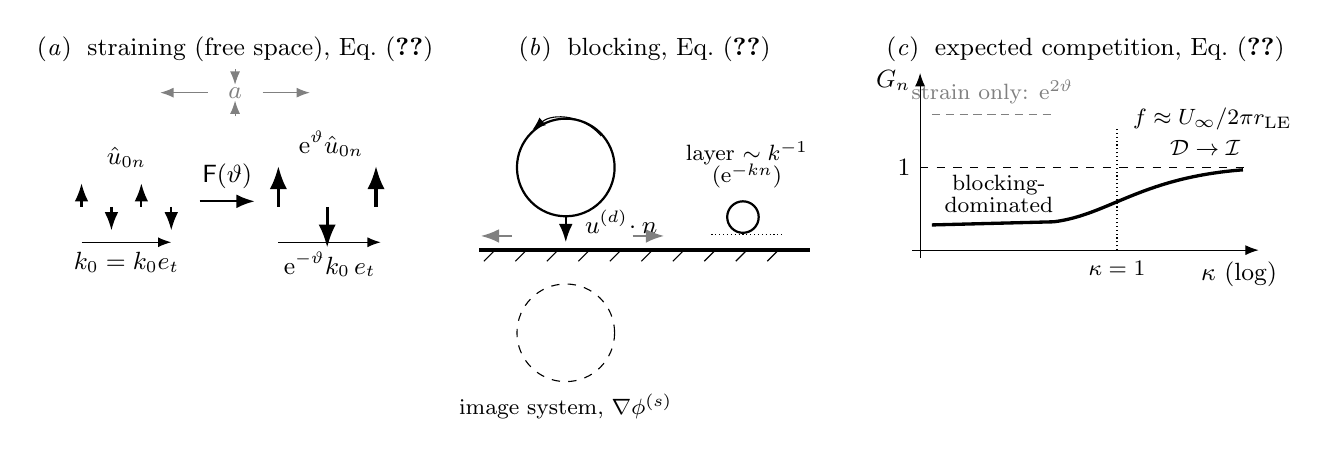
\begin{tikzpicture}[>=Latex, font=\small]
% ================= panel (a): free-space straining ======================
\begin{scope}[shift={(0,0)}]
  \node at (2.2,2.55) {(\textit{a})\; straining (free space), Eq.~(\ref{eq:worked_mode})};
  % strain cross
  \draw[->,gray] (1.85,2.0) -- (1.25,2.0);
  \draw[->,gray] (2.55,2.0) -- (3.15,2.0);
  \draw[->,gray] (2.2,2.30) -- (2.2,2.10);
  \draw[->,gray] (2.2,1.70) -- (2.2,1.90);
  \node[gray] at (2.2,2.0) {$a$};
  % BEFORE: short-wavelength gust, k0 along e_t, small u_n arrows
  \foreach \i/\s in {0/1,1/-1,2/1,3/-1}
    \draw[->,thick] ({0.25+0.38*\i},0.55) -- ++(0,{0.30*\s});
  \draw[->] (0.25,0.10) -- (1.39,0.10);
  \node[below] at (0.82,0.10) {$\boldsymbol{k}_0 = k_0\boldsymbol{e}_t$};
  \node at (0.82,1.18) {$\hat{u}_{0n}$};
  % mapping arrow
  \draw[->,thick] (1.75,0.62) -- (2.45,0.62);
  \node[above] at (2.10,0.65) {$\mathsf{F}(\vartheta)$};
  % AFTER: stretched wavelength, amplified u_n
  \foreach \i/\s in {0/1,1/-1,2/1}
    \draw[->,very thick] ({2.75+0.62*\i},0.55) -- ++(0,{0.52*\s});
  \draw[->] (2.75,0.10) -- (4.05,0.10);
  \node[below] at (3.40,0.10) {$\mathrm{e}^{-\vartheta}k_0\,\boldsymbol{e}_t$};
  \node at (3.42,1.35) {$\mathrm{e}^{\vartheta}\hat{u}_{0n}$};
\end{scope}
% ================= panel (b): blocking ==================================
\begin{scope}[shift={(5.3,0)}]
  \node at (2.1,2.55) {(\textit{b})\; blocking, Eq.~(\ref{eq:blocking})};
  % wall
  \draw[very thick] (0,0) -- (4.2,0);
  \foreach \xx in {0.2,0.6,...,4.0}
    \draw ({\xx},0) -- ({\xx-0.14},-0.14);
  % large eddy + cancelled normal velocity
  \draw[thick] (1.1,1.05) circle (0.62);
  \draw[->] (1.55,1.45) arc (40:130:0.62);
  \draw[->,thick] (1.1,0.43) -- (1.1,0.10);
  \node[anchor=west] at (1.22,0.36) {$\boldsymbol{u}^{(d)}\!\cdot\boldsymbol{n}$};
  % image (blocking) system
  \draw[dashed] (1.1,-1.05) circle (0.62);
  \node[below] at (1.1,-1.70) {\footnotesize image system, $\nabla\phi^{(s)}$};
  % tangential redistribution near wall
  \draw[->,gray,thick] (0.42,0.18) -- (0.02,0.18);
  \draw[->,gray,thick] (1.95,0.18) -- (2.35,0.18);
  % small eddy with thin blocking layer
  \draw[thick] (3.35,0.42) circle (0.20);
  \draw[densely dotted] (2.95,0.20) -- (3.85,0.20);
  \node[above,align=center] at (3.40,0.66)
        {\footnotesize layer $\sim k^{-1}$\\[-3pt]\footnotesize ($\mathrm{e}^{-kn}$)};
\end{scope}
% ================= panel (c): expected competition vs kappa =============
\begin{scope}[shift={(10.9,0)}]
  \node at (2.1,2.55) {(\textit{c})\; expected competition, Eq.~(\ref{eq:limits})};
  % axes
  \draw[->] (0,-0.1) -- (0,2.25);
  \node[left] at (0,2.15) {$G_n$};
  \draw[->] (-0.1,0) -- (4.3,0);
  \node[below] at (4.05,-0.02) {$\kappa$ (log)};
  % G = 1 reference
  \draw[dashed] (0,1.05) -- (4.2,1.05);
  \node[left] at (0,1.05) {$1$};
  % strain-only benchmark
  \draw[densely dashed,gray] (0.15,1.72) -- (1.7,1.72);
  \node[gray,above] at (0.92,1.74) {\footnotesize strain only: $\mathrm{e}^{2\vartheta}$};
  % kappa = 1 marker
  \draw[densely dotted] (2.5,0) -- (2.5,1.55);
  \node[below] at (2.5,-0.02) {\footnotesize $\kappa=1$};
  \node[anchor=west,align=left] at (2.58,1.66)
        {\footnotesize $f \approx U_\infty/2\pi r_{\mathrm{LE}}$};
  % expected G_n(kappa): suppressed plateau -> recovery to identity
  \draw[very thick]
        (0.15,0.32) -- (1.7,0.36)
        .. controls (2.4,0.45) and (2.8,0.92) .. (4.1,1.02);
  % regime labels
  \node[align=center] at (1.0,0.72)
        {\footnotesize blocking-\\[-3pt]\footnotesize dominated};
  \node[align=center] at (3.62,1.30) {\footnotesize $\mathcal{D}\to\mathcal{I}$};
\end{scope}
\end{tikzpicture}%
}
\caption{The two linear mechanisms of \S\,\ref{sec:framework_rdt} and
their expected competition. (\textit{a})~Free-space plane strain acting on
a tangentially aligned transverse gust stretches the wavelength and
amplifies the wall-normal amplitude by $\mathrm{e}^{\vartheta}$
(Eq.~\ref{eq:worked_mode}). (\textit{b})~Impermeability requires a
harmonic blocking correction whose layer thickness scales with the eddy
wavelength, suppressing the surface-normal component of large eddies and
redistributing energy tangentially (Eq.~\ref{eq:blocking};
\citealp{Hunt1973,HuntGraham1978}). (\textit{c})~Expected (schematic, not
measured) wall-normal gain: suppression below the strain-only benchmark
$\mathrm{e}^{2\vartheta}$ at $\kappa \lesssim 1$, recovery toward the
identity at $\kappa \gg 1$, crossover at $\kappa = \mathcal{O}(1)$
(Eq.~\ref{eq:limits}).}
\label{fig:framework_mechanisms}
\end{figure}
The two linear mechanisms thus act on the wall-normal component with
opposite sign: straining amplifies it, cf. (\ref{eq:worked_mode}), and
blocking suppresses it, cf. (\ref{eq:blocking}) \emph{ff}. Their relative
weight is controlled by the eddy-to-body-scale ratio, which for the airfoil
nose we write as $\kappa = k\,r_{\mathrm{LE}}$. The transposition of the
cylinder result to the airfoil nose --- with $r_{\mathrm{LE}}$, rather than
chord or thickness, as the controlling geometric scale --- is a hypothesis
of the present work. It is consistent with, though not established by, the
documented sensitivity of high-frequency leading-edge noise to nose
geometry \citep{Gill2013,DevenportStaubsGlegg2010} and with the success of
rapid-distortion corrections applied to measured upwash spectra
\citep{deSantana2016,dosSantos2023}. Verifying it, and locating the
crossover, is one task of the diagnostics defined in
\S\,\ref{sec:framework_observables}. The quantitative implication of
(\ref{eq:worked_mode}) is worth stating: where suppression of the
wall-normal component is observed at large scales, the blocking
contribution does not merely exceed the strain contribution --- it must
overcome an exponential amplification $\mathrm{e}^{2\vartheta}$, so that
the measured deficit underestimates the blocking effect in isolation.

\subsection{Dimensionless groups, integrated strain, and limiting regimes}
\label{sec:framework_groups}

Two dimensionless groups govern the linear problem. The first compares the
turbulent scale with the geometric scale of the nose,
\begin{equation}
  \kappa = k\,r_{\mathrm{LE}},
  \qquad k = \|\boldsymbol{k}\|.
  \label{eq:kappa}
\end{equation}
The second is the strain accumulated along the mean trajectory
$\boldsymbol{X}(t')$ terminating at the station $\theta$ on
$\mathcal{S}_{\mathrm{LE}}$,
\begin{equation}
  \vartheta(\theta)
  = \int_{0}^{\tau_{\mathrm{t}}}
    a\big(\boldsymbol{X}(t')\big)\,\mathrm{d}t'.
  \label{eq:vartheta}
\end{equation}
Two exact kinematic facts fix its magnitude and structure. First, for
plane flow the integrated strain along the symmetry streamline is
expressible in closed form: a material element convecting along a
streamline on which the speed falls from $U_1$ to $U_2$ is compressed
streamwise by the factor $U_2/U_1$ and extended laterally by $U_1/U_2$, so
that
\begin{equation}
  \vartheta\big|_{\theta=0}
  = \ln\!\frac{U_\infty}{U(\delta_n)},
  \label{eq:vartheta_exact}
\end{equation}
where $U(\delta_n)$ is the mean speed at the sampling offset on the
stagnation line. The integrated strain therefore diverges logarithmically
as the stagnation point is approached and is regularised by the finite
offset $\delta_n$; equivalently, $\vartheta$ is largest on the stagnation
line and decreases with $|\theta|$ as trajectories accelerate around the
nose, which is the kinematic origin of the azimuthal dependence carried by
$\mathcal{D}$ in (\ref{eq:operator}). Secondly, an elementary
potential-flow estimate fixes the local strain rate: for irrotational flow
past a circular cylinder of radius $r_{\mathrm{LE}}$ the tangential strain
rate at the stagnation point is $2U_\infty/r_{\mathrm{LE}}$, so that
$a = \mathcal{O}(U_\infty/r_{\mathrm{LE}})$, concentrated within a region
of extent $\mathcal{O}(r_{\mathrm{LE}})$ around the nose. The residence
time of a parcel in that region is
$\mathcal{O}(r_{\mathrm{LE}}/U_\infty)$, consistent with
$\vartheta = \mathcal{O}(1)$ off the stagnation line and larger on it,
per (\ref{eq:vartheta_exact}).

The operator structure then implies two limiting regimes, stated as
expectations to be tested rather than as established results for this
geometry:
\begin{equation}
\begin{aligned}
\kappa \lesssim 1:\quad
&\mathcal{D} \;\text{far from}\; \mathcal{I},
\qquad
\text{blocking-dominated for the normal component},
\\
\kappa \gg 1:\quad
&\mathcal{D} \to \mathcal{I}.
\end{aligned}
\label{eq:limits}
\end{equation}
The first limit follows from the blocking analysis: modes with wavelengths
exceeding $r_{\mathrm{LE}}$ cannot satisfy impermeability without a
blocking correction that pervades the entire pre-impact region, and their
surface-normal content is suppressed there notwithstanding the
$\mathrm{e}^{2\vartheta}$ strain amplification of
(\ref{eq:worked_mode}). The second limit reflects three compounding
facts: the blocking layer of a mode of wavenumber $k$ has thickness
$\mathcal{O}(k^{-1})$ and so, for $k\delta_n \gg 1$, lies below the
sampling surface; the strain accumulated by a small, rapidly convected
eddy during its $\mathcal{O}(r_{\mathrm{LE}}/U_\infty)$ residence in the
strain region is small; and the rapid-distortion condition
(\ref{eq:rdt_condition}) itself fails at small scales, where fast
turnover restores the upstream statistics --- so the identity limit is
approached partly for reasons outside linear theory. The crossover is
expected at $\kappa = \mathcal{O}(1)$, identifying $r_{\mathrm{LE}}$ as
the geometric filter separating strongly and weakly distorted classes of
motion.

\subsection{Observable projections, frequency--wavenumber assignment, and
identifiability}
\label{sec:framework_observables}

The data to be presented are pointwise frequency spectra and cross-plane
statistics on the two surfaces. The diagnostics are defined now, as
projections of $\mathcal{D}$, so that the results sections evaluate
pre-declared quantities.

The primary diagnostic is the component-wise spectral gain
\begin{equation}
  G_q(f)
  = \frac{\Phi^{\mathrm{LE}}_{qq}(f)}{\Phi^{\infty}_{qq}(f)},
  \qquad q \in \{u,v,w,p\}
  \quad\text{(no summation)},
  \label{eq:gain}
\end{equation}
a ratio of like-component power spectral densities. Departures of $G_q$
from unity measure the amplitude of the transformation at each scale;
inequality among the $G_q$ at fixed $f$ is the signature that the mapping
is tensorial, i.e. not expressible as
$\Phi^{\mathrm{LE}} = \alpha(f)\,\Phi^{\infty}$ for any scalar
$\alpha(f)$. Because (\ref{eq:gain}) is already a ratio of power spectral
densities, any acoustic quantity \emph{linear} in the incident spectrum
--- such as the far-field pressure spectral density of Amiet-type models,
which is proportional to the incident upwash spectrum
\citep{Amiet1975} --- inherits the factor $G$ linearly, not
quadratically; the corresponding level error is $10\log_{10}G$ decibels.

Azimuthal structure is resolved by projecting the midspan-plane velocity
components onto the cylindrical frame of \S\,\ref{sec:framework_states},
\begin{equation}
  u_r = u\cos\theta + v\sin\theta,
  \qquad
  u_\theta = -\,u\sin\theta + v\cos\theta,
  \qquad
  u_z = w,
  \label{eq:projection}
\end{equation}
an orthogonal rotation in the $(x,y)$ plane which preserves the in-plane
trace,
\begin{equation}
  \Phi_{uu} + \Phi_{vv} = \Phi_{rr} + \Phi_{\theta\theta},
  \qquad
  \Phi_{zz} = \Phi_{ww},
  \label{eq:trace}
\end{equation}
so that any inequality between $\Phi_{rr}$ and $\Phi_{\theta\theta}$
reflects genuine directional redistribution rather than a frame artefact.
The azimuthally resolved distortion and its rotation-invariant reductions
are
\begin{gather}
  \Delta_{qq}(St_c,\theta)
  = \log_{10}
    \frac{\widetilde{\Phi}^{\mathrm{LE}}_{qq}(St_c,\theta)}
         {\widetilde{\Phi}^{\infty}_{qq}(St_c,\theta)},
  \qquad q \in \{r,\theta\},
  \qquad
  \widetilde{\Phi}_{qq} = St_c\,\Phi_{qq},
  \label{eq:delta}
  \\[2pt]
  G_\perp(St_c,\theta)
  = \frac{\widetilde{\Phi}^{\mathrm{LE}}_{rr}
        + \widetilde{\Phi}^{\mathrm{LE}}_{\theta\theta}}
         {\widetilde{\Phi}^{\infty}_{rr}
        + \widetilde{\Phi}^{\infty}_{\theta\theta}},
  \qquad\quad
  \chi
  = \frac{\Phi_{rr} - \Phi_{\theta\theta}}
         {\Phi_{rr} + \Phi_{\theta\theta}},
  \qquad
  \Delta\chi = \chi^{\mathrm{LE}} - \chi^{\infty},
  \label{eq:tracegain_chi}
\end{gather}
with $St_c = fc/U_\infty$. By (\ref{eq:trace}), $G_\perp$ is invariant
under rotations in the projection plane and isolates the net in-plane
energy change, while $\chi \in [-1,1]$ isolates directional
redistribution independently of energy level. The single-point
counterpart of these scale-resolved diagnostics is the trajectory of
$(III,-II)$ along the approach, which records the structural
transformation integrated over all scales; the linear-theory reference
for that trajectory follows from
(\ref{eq:production_local}): a dominant plane strain acting on a state
with one dominant eigenvalue drives motion along the axisymmetric branch
(\ref{eq:lumley_boundary}), and pressure--strain redistribution --- absent
from (\ref{eq:rdt_structure}) in its congruence form --- is the
established mechanism for departures from it
\citep{SpezialeSarkarGatski1991,DurbinReif2017}.

Comparison with the wavenumber-space theory requires assigning a
wavenumber to each measured frequency. Under frozen convection
\citep{Taylor1938}, a point frequency spectrum and the streamwise
wavenumber spectrum are related by
$\Phi_{qq}(f) = (2\pi/U_c)\,E_{qq}(k_x)$ evaluated at
$k_x = 2\pi f/U_c$, which motivates the assignment
\begin{equation}
  \kappa(f) = \frac{2\pi f\,r_{\mathrm{LE}}}{U_c(f)},
  \label{eq:kappa_f}
\end{equation}
with $U_c(f)$ the convection velocity estimated from the phase of
streamwise cross-spectra between adjacent upstream probes. This step
carries known caveats, stated as limitations rather than resolved: frozen
convection is least secure precisely where the distortion is strongest,
since the mean flow decelerates and the convection velocity is
scale-dependent in inhomogeneous turbulence
\citep{WyngaardClifford1977,DelAlamoJimenez2009}. Accordingly
(\ref{eq:kappa_f}) is applied with $U_c$ evaluated on the upstream side,
$\kappa$ values quoted near the leading edge are nominal, and no
conclusion below rests on the precise location of the
$\kappa = \mathcal{O}(1)$ crossover --- only on its existence and on the
component ordering across it. With $U_c \approx U_\infty$,
(\ref{eq:kappa_f}) places $\kappa = 1$ at
$f \approx U_\infty/(2\pi r_{\mathrm{LE}})$, equivalently
$St_c \approx c/(2\pi r_{\mathrm{LE}})$, a single arithmetic link that
ties the frequency-domain gains (\ref{eq:gain}) and the Strouhal-domain
maps (\ref{eq:delta}) to a common scale.

Finally, identifiability. By the solenoidality constraint
(\ref{eq:solenoidal}), the spectral tensor at each
$(\boldsymbol{k},\omega)$ is a $2\times2$ Hermitian positive
semi-definite matrix on the transverse subspace, carrying four real
degrees of freedom; a general real-linear, realisability-preserving map of
such matrices carries of order sixteen real parameters at each
$(\boldsymbol{k},\vartheta,\theta)$. The diagnostics
(\ref{eq:gain})--(\ref{eq:tracegain_chi}) constrain a handful of scalar
combinations: the diagonal action in two frames, and two
rotation-invariant in-plane reductions. They do not constrain the
components of $\mathcal{D}_{ijmn}$ that generate or destroy cross-spectra
($\Phi_{ij}$, $i\ne j$), nor any phase information, and they sample
$\mathcal{S}_{\mathrm{LE}}$ on a single offset surface rather than
resolving the $\mathrm{e}^{-kn}$ wall-normal structure of the blocking
layer. The full reconstruction of
$\mathcal{D}_{ijmn}(\kappa,\vartheta;\theta)$ would require co-spectral
measurements in a consistently surface-aligned frame and is beyond the
scope of this paper. Within these limits, the linear framework yields
three falsifiable expectations that organise the results:
(i)~at $\kappa \lesssim 1$ the gains are unequal, with the wall-normal
(radial) component the most strongly suppressed --- the blocking
signature, made quantitative by the observation following
(\ref{eq:worked_mode}) that suppression there implies blocking strong
enough to overcome an $\mathrm{e}^{2\vartheta}$ strain amplification;
(ii)~the transition between distorted and undistorted behaviour occurs at
$\kappa = \mathcal{O}(1)$ in every component, at the frequency fixed by
(\ref{eq:kappa_f}); and
(iii)~the invariant-space trajectory follows the axisymmetric branch
(\ref{eq:lumley_boundary}) under the dominant plane strain, any excursion
off that branch --- in particular toward $III<0$ --- constituting direct
evidence of contributions, such as pressure--strain redistribution, beyond
the linear operator (\ref{eq:rdt_structure}).

% =========================================================================
% Section 3 — Numerical method and computational set-up
% Target: Journal of Fluid Mechanics (natbib, \citep / \citet).
%
% PLACEHOLDERS: every value not verifiable from the conference paper or
% the simulation context is written as \tbd{...} and listed in the audit.
% Define in the preamble while drafting:
% and delete the command once all values are filled.
%
% ADOPTED RESOLUTIONS (flagged, not silent):
%   Re_c = 5.1e5  -- consistent with U=20 m/s, c=0.4 m in air; the 1.1e6
%                    in the journal draft is dimensionally inconsistent
%                    with those values. CONFIRM operating point.
%   x_LE = 0.875 m -- consistent with x* = -2.19 grid station and the
%                    495+380 mm dimension chain in Fig. 3.
%   Projection plane: midspan (x,y), matching §2.6. CONFIRM vs scripts.
% =========================================================================

\section{Numerical method and computational set-up}
\label{sec:method}

\subsection{Lattice Boltzmann solver and turbulence modelling}
\label{sec:method_solver}

The simulations are performed with the lattice Boltzmann method (LBM)
implemented in the solver ProLB (version 3.3.1). The method evolves
particle distribution functions $f_i(\boldsymbol{x},t)$ on a Cartesian
lattice according to
\begin{equation}
  f_i(\boldsymbol{x} + \boldsymbol{\xi}_i\Delta t,\, t + \Delta t)
  = f_i(\boldsymbol{x},t) + \Omega_i(\boldsymbol{x},t),
  \label{eq:lbm}
\end{equation}
where $\boldsymbol{\xi}_i$ are the discrete lattice velocities,
$\Delta t$ the time step, and $\Omega_i$ the collision operator;
density and momentum are recovered as the zeroth and first moments of
$f_i$. The collision operator is the hybrid recursive regularised
Bhatnagar--Gross--Krook (HRR-BGK) model of \citet{Jacob2018}, which
combines a recursive regularisation of the non-equilibrium distributions
with a hybrid evaluation of the velocity-gradient contributions, providing
numerical stability at high Reynolds number while retaining the low
intrinsic dissipation and dispersion that make the LBM attractive for
time-domain aeroacoustics, in which hydrodynamic structures and acoustic
propagation are resolved within a single framework. \textcolor{teal}{The simulation of
grid-generated turbulence by lattice Boltzmann methods has been validated
against classical wind-tunnel data by \citet{Djenidi2006}.}

Subgrid-scale motions are represented by a large-eddy simulation (LES)
closure through an effective viscosity,
\begin{equation}
  \nu_{\mathrm{eff}} = \nu + \nu_{\mathrm{turb}},
  \label{eq:visc}
\end{equation}
with $\nu_{\mathrm{turb}}$ obtained from a Smagorinsky-type model
\citep{Smagorinsky1963} with dynamic evaluation of the model coefficient.
Near-wall behaviour is represented by a logarithmic wall model applied at
the first off-wall cell, incorporating corrections for streamwise pressure
gradient and surface curvature; the first-cell-centre height satisfies
$y^+ = \mathcal{O}(1)$ in the stagnation region
%% TODO: a referee may query the combination "wall model" + y+ = O(1)
%% (wall models are usually motivated by y+ >> 1). One clarifying sentence
%% on the role of the wall model at this resolution -- taken from the
%% ProLB documentation or the solver-team praxis -- would pre-empt this.
. Wall-model-based broadband-noise predictions with this methodology have
    been benchmarked within the BANC framework \citep{Herr2015}.

\subsection{Computational configuration and turbulence generation}
\label{sec:method_configuration}

% =====================================================================
% Values without flags: published AIAA/CEAS 2026 conference paper.
% [VALUE TO BE CONFIRMED]: absent from it; supply from run records.
% Fixed here: conference figure caption places the LE at x/c = 1.875
% (legacy 0.75 m configuration); correct value is x = 0.875 m.
% A-priori kinematic estimates (a, tau, vartheta) are derived purely
% from the configuration and are admissible in a methods section.
% NO measured turbulence quantities appear here.
% =====================================================================

\subsubsection{Geometry and coordinate system}

The computational arrangement reproduces the canonical configuration for
the study of turbulence--airfoil interaction: a passive
turbulence-generating grid placed upstream of a NACA~0012 airfoil held at
zero geometric incidence. A global Cartesian frame is adopted in which
$x$ denotes the streamwise, $y$ the transverse and $z$ the spanwise
direction, with the origin located in the plane of the turbulence grid.
The airfoil leading edge lies at $x_{\mathrm{LE}} = 0.875$~m, that is,
$2.19$ chord lengths downstream of the grid. Positions referenced to the
airfoil are expressed throughout via the shifted coordinate
\begin{equation}
  x^{\star} = \frac{x - x_{\mathrm{LE}}}{c},
  \label{eq:xstar_def}
\end{equation}
so that the grid plane corresponds to $x^{\star} = -2.19$ and the leading
and trailing edges to $x^{\star} = 0$ and $x^{\star} = 1$, respectively.

The airfoil has chord $c = 0.400$~m and occupies the full lateral extent
of the domain, with span $L_z = 0.800$~m, giving an aspect ratio
$L_z/c = 2$. This span was selected so that the largest energy-containing
structures of the incident turbulence decorrelate within the
computational span, a requirement for the spanwise statistics near the
leading edge to be free of artificial periodic (or wall-induced)
self-correlation; whether the chosen span satisfies this requirement is
verified a posteriori in \S\ref{sec:midspan_TI_corr_spectra}. For the
NACA~0012 section, the maximum thickness is $t = 0.12\,c = 48$~mm and
the geometric leading-edge radius follows from the thickness ratio
$t_c = 0.12$ as
\begin{equation}
  r_{\mathrm{LE}} = 1.1019\,t_c^{2}\,c \approx 6.3~\mathrm{mm},
  \label{eq:rLE_def}
\end{equation}
\citep{AbbottDoenhoff1959}, so that
$r_{\mathrm{LE}}/c = 1.6\times10^{-2}$.

\subsubsection{Non-dimensional parameters and characteristic scales}

The leading-edge radius constitutes the geometric inner scale of the
interaction problem and enters the analysis through the dimensionless
wavenumber
\begin{equation}
  \kappa = k\,r_{\mathrm{LE}},
  \label{eq:kappa_def}
\end{equation}
which compares the scale of an incident turbulent structure with the
scale of the nose geometry it encounters. The chord-based Strouhal
number, $St_c = fc/U_{\infty}$, provides the complementary outer-scale
frequency parameter. Throughout this paper the symbol $\kappa$ is
reserved exclusively for $k\,r_{\mathrm{LE}}$; streamwise distances
scaled by the nose radius are written $x/r_{\mathrm{LE}}$, and the
azimuthal coordinate on the nose-conforming sampling surfaces is denoted
$\phi$, to avoid any collision of symbols.

The free-stream velocity is $U_{\infty} = 20$~m\,s$^{-1}$, corresponding
to a Mach number $M \approx 0.059$ and a chord-based Reynolds number
$Re_c = U_{\infty}c/\nu \approx 5.1\times10^{5}$; the implied kinematic
viscosity, $\nu \approx 1.6\times10^{-5}$~m$^{2}$\,s$^{-1}$, represents
air at approximately ambient conditions. At this Mach number the flow is
effectively incompressible at the level of the turbulence dynamics,
while the weakly compressible formulation of the solver
(\S\ref{sec:numerical}) retains the acoustic degrees of freedom.

Two kinematic scales follow directly from the configuration and are
recorded here because they parameterise the theoretical framework of
\S\ref{sec:3}. First, an ideal stagnation flow about a nose of radius
$r_{\mathrm{LE}}$ possesses the characteristic strain-rate scale
\begin{equation}
  a \sim \frac{U_{\infty}}{2\,r_{\mathrm{LE}}}
    \approx 1.6\times10^{3}~\mathrm{s}^{-1},
  \label{eq:strain_scale}
\end{equation}
and, second, the convection time across one nose radius is
$\tau \sim r_{\mathrm{LE}}/U_{\infty} \approx 3.2\times10^{-4}$~s, so
that the a~priori estimate of the integrated distortion parameter is
\begin{equation}
  \vartheta = a\tau = \mathcal{O}(1/2).
  \label{eq:vartheta_estimate}
\end{equation}
These are geometric estimates, independent of the turbulence realised in
the computation; the strain field actually established in the stagnation
region, and the validity of the rapid-distortion approximation that
Eq.~(\ref{eq:vartheta_estimate}) presupposes, are assessed from the data
in \S\ref{sec:results}.

\subsubsection{Computational domain and boundary conditions}

The domain extends [VALUE TO BE CONFIRMED] upstream of the turbulence
grid and [VALUE TO BE CONFIRMED] downstream of the trailing edge, with a
transverse extent of [VALUE TO BE CONFIRMED] in $y$, corresponding to a
geometric blockage of the airfoil section of
[VALUE TO BE CONFIRMED]\,\%. The streamwise extents are dictated by two
competing requirements: the inflow boundary must be sufficiently remote
that the imposed uniform inflow does not constrain the development of
the grid wakes, while the outflow must be far enough downstream that the
wake of the airfoil leaves the region of interest without upstream
contamination. The spanwise boundary condition is
[VALUE TO BE CONFIRMED: periodic or slip]. At all remaining far-field
boundaries, characteristic non-reflecting conditions are combined with
sponge layers of thickness [VALUE TO BE CONFIRMED], in which the
fluctuating fields are progressively damped toward the imposed far-field
state; this treatment suppresses the spurious reflection of both
hydrodynamic and acoustic disturbances, the latter being of particular
concern for a compressible time-domain method in which outgoing waves
are explicitly resolved.
% Old working notes give [-5c, x_LE+10c], y = +-0.6 m, sponge over
% [x_LE+8c, x_LE+10c] -- superseded 0.75 m / 40 m/s configuration.
% Do not reuse without confirmation.

\subsubsection{Turbulence generation}

Turbulence is generated by an explicitly resolved passive grid rather
than by a synthetic inflow condition. This choice is deliberate and
central to the purpose of the study. Synthetic methods prescribe the
spectral content and componentality of the inflow by construction and
therefore presuppose precisely the statistical state whose
transformation is under investigation; an explicitly resolved grid, by
contrast, produces an incident field that carries the spatial structure,
inter-component anisotropy and decay history of physical grid turbulence
\citep{ComteBellotCorrsin1971,Roach1987}, at the cost of leaving the
inflow state to be determined empirically rather than imposed. No
assumption of homogeneity or isotropy is made at any point; the
statistical state of the field arriving at the airfoil is established
from the data in \S\ref{sec:midspan_TI_corr_spectra} and serves there as
the upstream reference state $\Phi^{\infty}_{ij}$ of the distortion
analysis.

The grid is a biplane arrangement of square bars
[CONFIGURATION DETAIL TO BE CONFIRMED] with mesh size
$M_g = $ [VALUE TO BE CONFIRMED], bar width
$d_g = $ [VALUE TO BE CONFIRMED] and solidity
\begin{equation}
  \sigma = \frac{d_g}{M_g}\left(2 - \frac{d_g}{M_g}\right)
         = [\mathrm{VALUE~TO~BE~CONFIRMED}],
  \label{eq:solidity}
\end{equation}
chosen below the threshold $\sigma \lesssim 0.4$ above which grid wakes
are known to coalesce into unstable jets and the downstream field loses
spatial uniformity \citep{Corrsin1963}. The grid-to-leading-edge
separation of $2.19\,c = [\mathrm{VALUE~TO~BE~CONFIRMED}]\,M_g$ reflects
the classical compromise of turbulence-interaction experiments: the
development length must be long enough, in grid-mesh units, for the
discrete bar wakes to merge and break down into a spatially
decorrelated broadband field --- conventionally
$x/M_g \gtrsim 10$--$20$ \citep{ComteBellotCorrsin1971} --- yet short
enough that the energy-containing scales remain energetic on arrival,
in particular over the range $\kappa \lesssim 1$ in which the strongest
interaction with the nose geometry is anticipated on dimensional
grounds (Eq.~\ref{eq:kappa_def}).
% If the nozzle (exit plane near x* = -0.95 in the project records) is
% part of the final configuration, insert here a geometry-only
% description: exit position, exit dimensions, contraction ratio.
% No statement about its effect on statistics -- that is results.
% [CONFIGURATION ITEM TO BE CONFIRMED]

\subsubsection{Spatial resolution}

The lattice is block-refined, with the finest resolution concentrated in
two regions: around the bars of the turbulence grid, where the wakes
that seed the turbulence must be resolved at their origin, and around
the airfoil nose, where the strongest mean-flow gradients of the
configuration occur over distances of order $r_{\mathrm{LE}}$. The
refinement criterion is formulated in terms of the scientific objective
rather than a wall-based quantity alone: structures at the geometric
crossover scale, $\kappa = \mathcal{O}(1)$, i.e.\ wavelengths
$\lambda = 2\pi r_{\mathrm{LE}} \approx 40$~mm and below, must be
resolved by at least [VALUE TO BE CONFIRMED] lattice points per
wavelength throughout the region traversed between the upstream
reference surfaces and the nose. The finest lattice spacing is
$\Delta x_{\min} = $ [VALUE TO BE CONFIRMED], corresponding to
$r_{\mathrm{LE}}/\Delta x_{\min} = $ [VALUE TO BE CONFIRMED] cells
across the nose radius, and the first off-wall cell in the stagnation
region lies at $y^{+} = \mathcal{O}(1)$ as required by the wall
treatment described in \S\ref{sec:numerical}. The complete mesh
comprises approximately $557\times10^{6}$ fluid nodes
[VALUE TO BE CONFIRMED], distributed over
[VALUE TO BE CONFIRMED] refinement levels.

\subsubsection{Time advancement, statistical sampling and record length}

The time step is fixed by the acoustic Courant condition of the lattice
Boltzmann scheme at the finest refinement level,
$\Delta t = $ [VALUE TO BE CONFIRMED], and the simulation is advanced
for a total of [VALUE TO BE CONFIRMED] flow-through times
$T_{\mathrm{ft}} = c/U_{\infty} = 0.02$~s, of which the first
[VALUE TO BE CONFIRMED] are discarded to eliminate the initial
transient associated with the establishment of the grid wakes and the
airfoil boundary layers. Statistical stationarity of the retained
record is verified by comparison of statistics over its first and
second halves; the result of this check is reported alongside the
corresponding quantities in \S\S\ref{sec:results}--\ref{sec:invariants}.

Velocity and pressure time series are recorded synchronously, at a
sampling rate of [VALUE TO BE CONFIRMED], at the vertices of the
sampling surfaces and along the probe lines described below. All
spectral estimates employ a frequency resolution
$\Delta f = U_{\infty}/(10c) = 5$~Hz, chosen to resolve the range
$St_c \in [0.1,\,200]$: the lower bound encompasses the largest
energy-containing scales expected from the grid spacing, while the
upper bound extends well beyond the frequency at which
$\kappa = \mathcal{O}(1)$ for any plausible convection velocity, so
that the geometric crossover region is bracketed with margin on both
sides.

Three families of recording locations are employed: (i) a
one-dimensional midspan probe line at fixed $(y,z)$ spanning the full
streamwise extent between grid and wake, on which mean profiles,
Reynolds stresses and anisotropy invariants are evaluated as functions
of $x^{\star}$; (ii) three planar patches located between the grid and
the airfoil, which establish the upstream reference state and, through
their mutual streamwise separation, permit an estimate of the
convection velocity from cross-spectral phase; and (iii) a
geometry-matched pair of toroidal surfaces of identical topology
conforming to the nose, one offset upstream and one enclosing the
pre-impact region. The geometric construction of these surfaces, and
the rationale for comparing like-with-like topologies, are given in
\S\ref{sec:sampling}; the spectral-estimation procedure, including the
robust patch aggregation and the reliability thresholds applied to all
spectral ratios, is given in \S\ref{sec:methodology_gain}.
% Planar patch coordinates per the analysis records:
% x = 0.435, 0.460, 0.475 m (x* = -1.10, -1.04, -1.00).
% [POSITIONS TO BE CONFIRMED] -- the conference paper instead says "one
% leading-edge radius upstream", inconsistent with these coordinates;
% resolve before submission.

\begin{table}
  \begin{center}
  \def~{\hphantom{0}}
  \begin{tabular}{lll}
    Quantity & Symbol & Value \\[3pt]
    Airfoil section                  & ---                & NACA~0012, zero incidence \\
    Chord                            & $c$                & $0.400$~m \\
    Span                             & $L_z$              & $0.800$~m \quad ($L_z/c = 2$) \\
    Leading-edge radius              & $r_{\mathrm{LE}}$  & $6.3$~mm \quad ($r_{\mathrm{LE}}/c = 1.6\times10^{-2}$) \\
    Grid--leading-edge separation    & $x_{\mathrm{LE}}$  & $0.875$~m \quad ($2.19\,c$) \\
    Free-stream velocity             & $U_{\infty}$       & $20$~m\,s$^{-1}$ \\
    Mach number                      & $M$                & $0.059$ \\
    Chord Reynolds number            & $Re_c$             & $5.1\times10^{5}$ \\
    Stagnation strain-rate scale     & $a$                & $\approx 1.6\times10^{3}$~s$^{-1}$ (Eq.~\ref{eq:strain_scale}) \\
    Distortion parameter (estimate)  & $\vartheta$        & $\mathcal{O}(1/2)$ (Eq.~\ref{eq:vartheta_estimate}) \\
    Grid mesh size                   & $M_g$              & [VALUE TO BE CONFIRMED] \\
    Grid solidity                    & $\sigma$           & [VALUE TO BE CONFIRMED] \\
    Finest lattice spacing           & $\Delta x_{\min}$  & [VALUE TO BE CONFIRMED] \\
    Fluid nodes                      & ---                & $\approx 557\times10^{6}$ [TO BE CONFIRMED] \\
    Record length                    & ---                & [VALUE TO BE CONFIRMED] $\times\, c/U_{\infty}$ \\
    Frequency resolution             & $\Delta f$         & $5$~Hz \quad ($St_c \in [0.1, 200]$) \\
  \end{tabular}
  \caption{Summary of the computational configuration. Bracketed entries
  are stated in the simulation records and reproduced here pending
  confirmation.}
  \label{tab:config}
  \end{center}
\end{table}

\subsection{Computational configuration and turbulence generation}
\label{sec:method_configuration}
% =========================================================================
% fig_domain3d.tex — 3D schematic of the computational domain (§3.2)
% Cavalier projection: (x,y,z) -> (x + 0.42 z, y + 0.26 z).
% All coordinates absolute; \pxy{x}{y}{z} is the projection macro.
% Requires: tikz (calc, arrows.meta), xcolor, amsmath. NOT to scale —
% stated in the caption; true dimensions appear as callouts.
%
% Splice into §3.2 after the first paragraph:
%   "The configuration is summarised in figure~\ref{fig:domain3d}."
% =========================================================================
\begin{figure}
\centering
\newcommand{\pxy}[3]{({(#1)+0.42*(#3)},{(#2)+0.26*(#3)})}
\resizebox{\textwidth}{!}{%
\begin{tikzpicture}[>=Latex, font=\small, line join=round]
% ---------------- domain box (hidden edges light) --------------------
% corners: x in {-3.2,10.5}, y in {-2.2,2.2}, z in {0,2.2}
\draw[gray!50] \pxy{-3.2}{-2.2}{2.2} -- \pxy{10.5}{-2.2}{2.2}
               -- \pxy{10.5}{2.2}{2.2} -- \pxy{-3.2}{2.2}{2.2} -- cycle;
\draw[gray!50] \pxy{-3.2}{-2.2}{0} -- \pxy{-3.2}{-2.2}{2.2};
\draw[gray!50] \pxy{10.5}{-2.2}{0} -- \pxy{10.5}{-2.2}{2.2};
\draw[gray!50] \pxy{10.5}{2.2}{0}  -- \pxy{10.5}{2.2}{2.2};
\draw[gray!50] \pxy{-3.2}{2.2}{0}  -- \pxy{-3.2}{2.2}{2.2};
\draw[black]   \pxy{-3.2}{-2.2}{0} -- \pxy{10.5}{-2.2}{0}
               -- \pxy{10.5}{2.2}{0} -- \pxy{-3.2}{2.2}{0} -- cycle;
% ---------------- inflow ---------------------------------------------
\foreach \y in {-1.0,-0.35,0.35,1.0}
  \draw[->,thick,gray] \pxy{-4.05}{\y}{1.1} -- \pxy{-3.35}{\y}{1.1};
\node[gray,anchor=west] at \pxy{-3.05}{1.55}{1.1} {uniform inflow $U_\infty$};
% ---------------- turbulence grid at x = 0 ---------------------------
\foreach \z in {0.2,0.65,1.1,1.55,2.0}
  \draw[thick] \pxy{0}{-1.5}{\z} -- \pxy{0}{1.5}{\z};
\foreach \y in {-1.5,-1.0,-0.5,0,0.5,1.0,1.5}
  \draw[thick] \pxy{0}{\y}{0.2} -- \pxy{0}{\y}{2.0};
\node[anchor=south] at \pxy{-0.9}{2.45}{1.1} {turbulence grid ($x=0$)};
\draw[gray!70] \pxy{-0.75}{2.42}{1.1} -- \pxy{0}{1.6}{1.1};
% ---------------- nozzle contraction ----------------------------------
% top and bottom walls, front (z=0.2) solid, back (z=2.0) light
\draw[thick]    \pxy{0.3}{1.5}{0.2}  -- \pxy{2.2}{0.95}{0.2};
\draw[thick]    \pxy{0.3}{-1.5}{0.2} -- \pxy{2.2}{-0.95}{0.2};
\draw[gray!60]  \pxy{0.3}{1.5}{2.0}  -- \pxy{2.2}{0.95}{2.0};
\draw[gray!60]  \pxy{0.3}{-1.5}{2.0} -- \pxy{2.2}{-0.95}{2.0};
\draw[gray!60]  \pxy{0.3}{1.5}{0.2}  -- \pxy{0.3}{1.5}{2.0};
\draw[gray!60]  \pxy{0.3}{-1.5}{0.2} -- \pxy{0.3}{-1.5}{2.0};
% nozzle exit plane (dashed rectangle)
\draw[dashed]   \pxy{2.2}{-0.95}{0.2} -- \pxy{2.2}{0.95}{0.2}
             -- \pxy{2.2}{0.95}{2.0}  -- \pxy{2.2}{-0.95}{2.0} -- cycle;
\node[anchor=south] at \pxy{3.2}{2.45}{1.1} {nozzle exit};
\draw[gray!70] \pxy{3.1}{2.42}{1.1} -- \pxy{2.25}{1.05}{1.1};
\node at \pxy{1.25}{-1.85}{0.2} {nozzle};
% ---------------- planar patches P1, P2, P3 ---------------------------
\definecolor{cP1}{RGB}{34,160,80}
\definecolor{cP2}{RGB}{110,110,220}
\definecolor{cP3}{RGB}{225,120,20}
\foreach \xp/\cc/\nm in {2.45/cP1/P1, 2.70/cP2/P2, 2.95/cP3/P3}{
  \draw[\cc, thick, fill=\cc, fill opacity=0.13]
    \pxy{\xp}{-0.85}{0.35} -- \pxy{\xp}{0.85}{0.35}
    -- \pxy{\xp}{0.85}{1.85} -- \pxy{\xp}{-0.85}{1.85} -- cycle;
}
\node[anchor=west] at \pxy{0.45}{-2.40}{0}
  {\footnotesize upstream patches \textcolor{cP1}{P1}, \textcolor{cP2}{P2},
   \textcolor{cP3}{P3}\; (P3 $\to \Phi^{\infty}_{ij}$)};
% ---------------- NACA 0012 wing (extruded) ---------------------------
% chord c = 2.4 units, LE at x = 4.6; span z in [0.3, 1.9]
% y(x) = 2.4*0.6*poly(t), t in [0,1]
% back-face profile first (light), then connectors, then front face
\draw[gray!60]
  plot[domain=0:1,samples=70]
    ({4.6+2.4*\x+0.42*1.9},{1.44*(0.2969*sqrt(\x)-0.1260*\x-0.3516*\x*\x+0.2843*\x*\x*\x-0.1036*\x*\x*\x*\x)+0.26*1.9})
  -- plot[domain=1:0,samples=70]
    ({4.6+2.4*\x+0.42*1.9},{-1.44*(0.2969*sqrt(\x)-0.1260*\x-0.3516*\x*\x+0.2843*\x*\x*\x-0.1036*\x*\x*\x*\x)+0.26*1.9})
  -- cycle;
\draw[gray!70] \pxy{4.6}{0}{0.3} -- \pxy{4.6}{0}{1.9};   % LE line
\draw[gray!70] \pxy{7.0}{0}{0.3} -- \pxy{7.0}{0}{1.9};   % TE line
\draw[thick,fill=gray!15]
  plot[domain=0:1,samples=70]
    ({4.6+2.4*\x+0.42*0.3},{1.44*(0.2969*sqrt(\x)-0.1260*\x-0.3516*\x*\x+0.2843*\x*\x*\x-0.1036*\x*\x*\x*\x)+0.26*0.3})
  -- plot[domain=1:0,samples=70]
    ({4.6+2.4*\x+0.42*0.3},{-1.44*(0.2969*sqrt(\x)-0.1260*\x-0.3516*\x*\x+0.2843*\x*\x*\x-0.1036*\x*\x*\x*\x)+0.26*0.3})
  -- cycle;
\node[anchor=north] at \pxy{6.1}{-0.32}{0.3} {NACA 0012};
% ---------------- toroidal pre-impact patch (exaggerated) -------------
\definecolor{cTor}{RGB}{200,30,30}
\draw[cTor, very thick] ([shift={(100:0.24)}]{4.6+0.42*0.3},{0.26*0.3})
  arc (100:260:0.24);
\draw[cTor, very thick] ([shift={(100:0.24)}]{4.6+0.42*1.9},{0.26*1.9})
  arc (100:260:0.24);
\draw[cTor] ([shift={(100:0.24)}]{4.6+0.42*0.3},{0.26*0.3})
  -- ([shift={(100:0.24)}]{4.6+0.42*1.9},{0.26*1.9});
\draw[cTor] ([shift={(260:0.24)}]{4.6+0.42*0.3},{0.26*0.3})
  -- ([shift={(260:0.24)}]{4.6+0.42*1.9},{0.26*1.9});
\node[cTor, anchor=east, align=right] at \pxy{4.28}{-1.10}{0.3}
  {\footnotesize toroidal patch\\[-2pt]
   \footnotesize $\mathcal{S}_{\mathrm{LE}} \to \Phi^{\mathrm{LE}}_{ij}$};
\draw[cTor!70] \pxy{4.34}{-1.02}{0.3} -- \pxy{4.56}{-0.26}{0.3};
% ---------------- microphone array (midspan plane) --------------------
\draw[densely dotted] \pxy{5.8}{0}{1.1} circle (2.45);
\foreach \a in {15,55,95,140,220,265,305,345}
  \fill ([shift={(\a:2.45)}]{5.8+0.42*1.1},{0.26*1.1}) circle (1.6pt);
\node[anchor=west] at \pxy{7.95}{1.62}{1.1} {\footnotesize microphone array};
% ---------------- outlet / sponge annotation --------------------------
\node[anchor=west, align=left] at \pxy{10.75}{0.6}{1.1}
  {\footnotesize pressure outlet};
\node[anchor=west, align=left] at \pxy{10.75}{-0.1}{1.1}
  {\footnotesize non-reflecting +\\[-2pt]\footnotesize sponge layers\\[-2pt]
   \footnotesize (all outer faces)};
% ---------------- dimension callouts (front-bottom baseline) ----------
\newcommand{\dimtick}[1]{\draw \pxy{#1}{-2.45}{0} -- \pxy{#1}{-2.75}{0};}
\dimtick{-3.2}\dimtick{0}\dimtick{2.2}\dimtick{4.6}\dimtick{7.0}\dimtick{10.5}
\draw[<->] \pxy{-3.2}{-2.6}{0} -- \pxy{0}{-2.6}{0};
\node[below] at \pxy{-1.6}{-2.62}{0} {\footnotesize $15\,c$};
\draw[<->] \pxy{0}{-2.6}{0} -- \pxy{2.2}{-2.6}{0};
\node[below] at \pxy{1.1}{-2.62}{0} {\footnotesize $495$~mm};
\draw[<->] \pxy{2.2}{-2.6}{0} -- \pxy{4.6}{-2.6}{0};
\node[below] at \pxy{3.4}{-2.62}{0} {\footnotesize $380$~mm};
\draw[<->] \pxy{4.6}{-2.6}{0} -- \pxy{7.0}{-2.6}{0};
\node[below] at \pxy{5.8}{-2.62}{0} {\footnotesize $c=400$~mm};
\draw[<->] \pxy{7.0}{-2.6}{0} -- \pxy{10.5}{-2.6}{0};
\node[below] at \pxy{8.75}{-2.62}{0} {\footnotesize $20\,c$};
% lateral extent (left, outside)
\draw[<->] \pxy{-3.55}{-2.2}{0} -- \pxy{-3.55}{2.2}{0};
\node[rotate=90, above] at \pxy{-3.62}{0}{0} {\footnotesize $50\,c$};
% span (above wing, along z)
\draw[<->] \pxy{7.35}{0.45}{0.3} -- \pxy{7.35}{0.45}{1.9};
\node[anchor=south west] at \pxy{7.45}{0.55}{1.25} {\footnotesize $L_z = 2\,c$};
% ---------------- coordinate triad ------------------------------------
\draw[->,thick] \pxy{-2.7}{-1.7}{0.25} -- \pxy{-1.9}{-1.7}{0.25} node[right] {$x$};
\draw[->,thick] \pxy{-2.7}{-1.7}{0.25} -- \pxy{-2.7}{-0.9}{0.25} node[above] {$y$};
\draw[->,thick] \pxy{-2.7}{-1.7}{0.25} -- \pxy{-2.7}{-1.7}{1.15} node[above right] {$z$};
\end{tikzpicture}%
}
\caption{Three-dimensional schematic of the computational domain (not to
scale; true dimensions as callouts). Uniform inflow passes the passive
turbulence-generating grid at $x=0$ and the nozzle contraction; the
NACA\,0012 airfoil is mounted at zero incidence with its leading edge
$380$~mm downstream of the nozzle exit. The three planar patches P1--P3
sample the upstream state, with P3 providing the operational reference
$\Phi^{\infty}_{ij}$ (\S\,\ref{sec:method_states}); the toroidal patch
(radius exaggerated for visibility) wraps the leading edge across the
span and samples the pre-impact state $\Phi^{\mathrm{LE}}_{ij}$. The
microphone array lies in the midspan plane. Non-reflecting conditions
and sponge layers are applied on all outer faces.}
\label{fig:domain3d}
\end{figure}
The configuration reproduces an open-jet aeroacoustic test section. A
uniform inflow enters a nozzle whose exit plane is located $495$~mm
downstream of a passive turbulence-generating grid placed at $x = 0$; a
NACA\,0012 airfoil of chord $c = 0.4$~m and span $L_z = 0.8$~m is mounted
at zero geometric incidence with its leading edge at
$x_{\mathrm{LE}} = 0.875$~m, i.e. $2.19\,c$ downstream of the grid and
$380$~mm downstream of the nozzle exit. The geometric leading-edge radius
is $r_{\mathrm{LE}} \approx 6.3$~mm, consistent with the analytical value
$1.1019\,t^2 c = 0.0159\,c$ for a four-digit section of thickness ratio
$t = 0.12$. The free-stream velocity is $U_\infty = 20$~m\,s$^{-1}$,
giving a Mach number $M \approx 0.059$ and a chord-based Reynolds number
$Re_c = U_\infty c/\nu \approx 5.1\times10^{5}$.
%% FLAG: the working journal draft states 1.1e6 in the abstract, set-up
%% and conclusion; that value is inconsistent with U = 20 m/s, c = 0.4 m
%% in air. Confirm the operating point and make the manuscript uniform.
The turbulence-generating grid has mesh size
$M_g = \tbd{grid mesh size}$, bar thickness $d_g = \tbd{bar thickness}$ and solidity
$\sigma = \tbd{solidity}$. The computational domain extends
$\tbd{upstream extent}$ upstream of the grid and $20\,c$ downstream of
the airfoil, with a lateral extent of $50\,c$; the spanwise boundaries
are $\tbd{spanwise BC: periodic / frictionless}$, and non-reflecting
characteristic conditions combined with sponge layers are applied at all
far-field boundaries to suppress spurious acoustic reflections.

The grid--airfoil separation of $2.19\,c$ is chosen so that the
grid-generated turbulence attains a statistically developed, spatially
decorrelated state before reaching the airfoil while retaining
significant energy at the scales $\kappa \lesssim 1$ for which the
distortion of \S\,\ref{sec:framework} is expected to be strongest; at the
upstream reference location the turbulence intensities are
$u'_\infty/U_\infty = 4.1\%$ and $v'_\infty/U_\infty = 2.0\%$ with
$R_{11}/R_{22} = 4.2$ (patch-averaged values, \S\,\ref{sec:method_states}).
The statistics presented in
\S\S\,\ref{sec:flowfield}--\ref{sec:spectra} are accumulated over a
physical time $T = \tbd{record length}$ after the discarding of an
initial transient of $\tbd{transient}$ flow-through times.

\subsection{Instantiation of the two turbulence states}
\label{sec:method_states}

The abstract surfaces of \S\,\ref{sec:framework_states} are realised as
sampling patches on which velocity and pressure time series are recorded
at every surface vertex.

The upstream state is sampled on three parallel planar patches
P1--P3, normal to the mean flow and located at
$x = \tbd{x P1}, \tbd{x P2}, \tbd{x P3}$
%% DECISION POINT: two readings of the patch stations coexist in the
%% source material -- the conference Fig. 13 legends (x = 0.435, 0.460,
%% 0.475 m, i.e. inside the nozzle) and the working analysis (at/after
%% the nozzle exit, x* = -0.95 to -0.75). Take the values from the
%% post-processing scripts, not from either document.
, each of transverse extent $\tbd{patch extent}$ and
$N_v = \tbd{vertex count}$ vertices. Three planes rather than one serve
two purposes: their mutual collapse establishes the spectral stationarity
of the reference family, and their separation provides a local estimate
of the streamwise decay rate used below. The patch furthest downstream,
P3, defines the operational reference spectra $\Phi^{\infty}_{qq}(f)$.
The pre-impact state is sampled on a toroidal patch conformal to the
airfoil nose at a wall offset $\delta_n = \tbd{offset value}$
($\delta_n/r_{\mathrm{LE}} = \tbd{ratio}$), spanning azimuthal stations
$\theta \in [-100^\circ, 100^\circ]$
%% TODO: confirm the azimuthal extent against the patch definition; the
%% value above is read from the distortion maps of the conference paper.
and the full span. An intermediate planar patch one leading-edge radius
ahead of the nose is retained as a near-field control surface; it is
emphasised that this surface lies within the blocking zone of all eddies
with $\kappa \lesssim 1$ (\S\,\ref{sec:framework_rdt}) and therefore
cannot serve as the upstream reference. Velocities on the toroidal patch
are decomposed in the cylindrical frame of
\S\,\ref{sec:framework_states} by the midspan-plane rotation
(\ref{eq:projection}).
%% DECISION POINT: midspan-(x,y) projection adopted, matching §2.6 and
%% the published figure geometry; the working journal draft contains a
%% contradictory (v,w) version. Confirm against the analysis scripts.

The transit from P3 to the toroidal patch decomposes into two segments
with sharply different physics, and the distinction governs how the
operator of \S\,\ref{sec:framework_hypothesis} is evaluated from the
data. Over the first segment, of length
$\ell_\infty \approx \tbd{value}\,c \approx \tbd{value}\,r_{\mathrm{LE}}$
and transit time $\tau_1 = \ell_\infty/U_\infty \approx
\tbd{value}$~ms, the mean strain is negligible but the grid turbulence
decays freely; a preliminary estimate based on classical decay exponents
$u'^2 \propto x^{-n}$ with $n = 1.25$--$1.4$
\citep{ComteBellotCorrsin1971,Roach1987} gives a variance reduction by a
factor of $0.4$--$0.6$ ($2$--$4$~dB) over this segment, which is not
negligible against the measured gains. Over the second segment, the final
few leading-edge radii, the residence time is
$\mathcal{O}(r_{\mathrm{LE}}/U_\infty) \approx 0.3$~ms --- shorter than
the turnover time of the energy-containing eddies by more than an order
of magnitude for any integral scale exceeding a few millimetres --- so
that the rapid-distortion condition (\ref{eq:rdt_condition}) is
comfortably satisfied precisely where the strain and blocking act, while
free decay over this segment is negligible.

The measured transformation between P3 and the toroidal patch is
therefore a composition,
\begin{equation}
  \mathcal{D}_{\mathrm{total}}
  = \mathcal{D}(\boldsymbol{k},\vartheta;\theta)
    \circ
    \mathcal{D}_{\mathrm{decay}}(f),
  \label{eq:composition}
\end{equation}
in which only the first factor is the body-induced operator of
\S\,\ref{sec:framework}. To isolate it, the reference spectra are
extrapolated to the leading-edge station: the spectra
$\Phi_{qq}(f;x)$ at the midspan stations between the nozzle exit and the
onset of the blocking zone
($x^\star \in [\tbd{lo}, \tbd{hi}]$, chosen to exclude the nozzle-exit
signature on the upstream side and to remain at least one integral scale
ahead of the nose on the downstream side) are fitted, frequency by
frequency, to a power-law decay in $x$, and evaluated at
$x^\star = 0$ to define the baseline
\begin{equation}
  \widehat{\Phi}^{\infty}_{qq}(f)
  \;=\;
  \left[\Phi_{qq}(f;x)\right]_{\mathrm{extrapolated\ to\ }
  x = x_{\mathrm{LE}}\ \mathrm{in\ the\ absence\ of\ the\ airfoil}},
  \label{eq:baseline}
\end{equation}
i.e. the spectrum that would arrive at the leading-edge station were the
airfoil absent. The primary spectral gains of
\S\,\ref{sec:spectra} are computed against this baseline,
$G_q(f) = \Phi^{\mathrm{LE}}_{qq}(f)/\widehat{\Phi}^{\infty}_{qq}(f)$,
so that departures of $G_q$ from unity measure the body-induced
transformation alone; the raw, P3-referenced gains are reported alongside
for transparency, the difference between the two quantifying the decay
factor directly.
%% NOTE: this is the new methodological element relative to the
%% conference paper, motivated by the transit-length analysis. If the
%% per-station spectra are not yet computed, they are obtainable from the
%% existing midspan probe time series (the autocorrelation stations).
Two properties make the conclusions robust to the residual uncertainty of
the extrapolation: free decay is component-blind at leading order, so the
component-differential structure of $G_q$ --- the tensorial signature ---
is unaffected by the choice of baseline; and to the extent that decaying
grid turbulence returns toward isotropy, the correction raises the
wall-normal gain relative to the streamwise one, so that the wall-normal
suppression reported in \S\,\ref{sec:spectra} is, if anything,
conservative.

The framework parameters take the following values in this configuration.
The geometric crossover (\ref{eq:kappa_f}) with $U_c \approx U_\infty$
places $\kappa = 1$ at
$f_1 = U_\infty/(2\pi r_{\mathrm{LE}}) \approx 5.1\times10^{2}$~Hz,
equivalently $St_c = c/(2\pi r_{\mathrm{LE}}) \approx 10$, linking the
frequency-domain gains and the Strouhal-domain distortion maps to a
common scale; the corresponding wavelength, $2\pi r_{\mathrm{LE}} \approx
40$~mm, sets the resolution requirement of
\S\,\ref{sec:method_resolution}. The integrated strain on the stagnation
line follows from the exact kinematic relation
(\ref{eq:vartheta_exact}) as
$\vartheta|_{\theta=0} = \ln\!\big(U_\infty/U(\delta_n)\big)
= \tbd{value}$,
%% TODO: evaluate with the measured mean speed at the sampling offset;
%% the midspan profile suggests U(delta_n) of order 7-8 m/s, giving
%% vartheta ~ 0.9-1.0 and a strain-only benchmark e^{2 vartheta} ~ 6-7.
%% CONFIRM from the data before quoting.
so that the strain-only benchmark of \S\,\ref{sec:framework_rdt} is
$\mathrm{e}^{2\vartheta} = \tbd{value}$ for tangentially aligned gusts
arriving on the stagnation line.

\subsection{Spectral estimation and statistical convergence}
\label{sec:method_spectra}

At each patch vertex the temporal mean and the instantaneous
patch-averaged fluctuation are removed before spectral estimation,
\begin{equation}
  q''_j(t)
  = q_j(t) - \overline{q_j}
  - \frac{1}{N_v}\sum_{m=1}^{N_v}\big(q_m(t)-\overline{q_m}\big),
  \qquad q \in \{u,v,w,p\},
  \quad j = 1,\dots,N_v,
  \label{eq:patch_fluct}
\end{equation}
which suppresses spatially uniform, patch-scale contributions such as
slow facility-mode oscillations. One-sided spectra are computed at each
vertex by the Welch method \citep{Welch1967} with Hann windowing, $50\%$
overlap and segment length $\tbd{segment length}$ samples, giving a frequency
resolution $\Delta f = U_\infty/(10c) = 5$~Hz over the resolved range
$St_c \in [0.1, 200]$. The vertex spectra are aggregated by a median,
\begin{equation}
  \widetilde{\Phi}^{P}_{qq}(f)
  = \operatorname{median}_{j\in P}\big[\Phi^{(j)}_{qq}(f)\big],
  \label{eq:patch_spectrum}
\end{equation}
in preference to the arithmetic mean, because the vertex population
contains localised high-amplitude members associated with near-wall
intermittency and geometric clustering on the toroidal surface; the
median is robust to these without biasing the bulk of the distribution,
and the mean estimator was verified to preserve the same qualitative
trends. Statistical convergence is assessed in two ways: the record
length corresponds to $\tbd{value}$ integral time scales of the upstream
turbulence ($\tbd{value}$ Welch segments), and the segment-to-segment
scatter provides a confidence band on each spectrum which, propagated
through the ratio, yields the uncertainty estimate displayed with the
gains $G_q$ in \S\,\ref{sec:spectra}.
%% TODO: the conference paper asserts convergence without showing it; a
%% JFM referee will ask how converged a RATIO of spectra is. The
%% segment-bootstrap band proposed here is cheap and defuses the
%% objection; it requires only re-running the Welch aggregation.
The convection velocity $U_c(f)$ entering the frequency--wavenumber
assignment (\ref{eq:kappa_f}) is estimated from the phase slope of the
streamwise cross-spectrum between adjacent upstream probes
\citep{DelAlamoJimenez2009}. Finally, the gain diagnostics are
interpreted only where the reference spectrum exceeds a reliability
threshold of $\tbd{value}$
%% TODO: state the criterion actually used for the shaded regions
%% (e.g. a fixed margin above the high-frequency noise floor of the
%% upstream spectra); it must be DEFINED here, before any G_q figure.
above the numerical noise floor; frequencies failing this criterion are
shaded in the corresponding figures and excluded from interpretation.

\subsection{Resolution and validation}
\label{sec:method_resolution}

The lattice spacing is refined in successive embedded regions toward the
airfoil, with the finest resolution
$\Delta x_{\min} = \tbd{value}$ ($r_{\mathrm{LE}}/\Delta x_{\min}
= \tbd{value}$) in a region enclosing the nose and the toroidal patch,
so that the geometric crossover scale $2\pi r_{\mathrm{LE}} \approx
40$~mm is resolved by $\tbd{value}$ cells and the stagnation-region
velocity gradients of \S\,\ref{sec:framework_states} are captured
directly rather than modelled. In the grid-development region the
resolution is $\Delta x = \tbd{value}$, resolving the energy-containing
scales of the inflow; the dissipative range is represented by the LES
closure of \S\,\ref{sec:method_solver}, and the spectral tail beyond
$\kappa \approx \tbd{value}$ is excluded from interpretation by the
reliability criterion of \S\,\ref{sec:method_spectra}.
%% TODO: if a grid-refinement or sensitivity study exists (even partial),
%% summarise it here in two sentences; if not, the resolution argument
%% rests on the cell counts above plus the validation below.

The inflow turbulence is validated against classical grid-turbulence
behaviour: the streamwise decay of intensity and the growth of the
integral scale follow power laws with constants
$C_u = \tbd{value}$, $C_\Lambda = \tbd{value}$ and exponents within the
range established for static grids
\citep{ComteBellotCorrsin1971,Roach1987,Ertunc2010}, and the measured
upstream anisotropy ($u'_\infty > v'_\infty \approx w'_\infty$, with the
invariant state adjacent to the axisymmetric branch near the
one-component corner) is consistent with the documented large-scale
anisotropy of passive-grid turbulence \citep{ComteBellotCorrsin1971,
Ertunc2010}. The wall resolution satisfies $y^+ = \mathcal{O}(1)$ over
the nose region
%% TODO: quote the y+ map or its range over the toroidal-patch footprint.
, and the sponge layers were verified to suppress boundary reflections to
below $\tbd{value}$ of the incident amplitude across the resolved
frequency range.
%% TODO: replace with whatever reflection check exists; if none, delete
%% the clause rather than leave an unsupported claim.

\newpage
\subsection{Computational configuration and turbulence generation}
\label{sec:method_configuration}

% =====================================================================
% Values without flags: published AIAA/CEAS 2026 conference paper.
% [VALUE TO BE CONFIRMED]: absent from it; supply from run records.
% Fixed here: conference figure caption places the LE at x/c = 1.875
% (legacy 0.75 m configuration); correct value is x = 0.875 m.
% A-priori kinematic estimates (a, tau, vartheta) are derived purely
% from the configuration and are admissible in a methods section.
% NO measured turbulence quantities appear here.
% =====================================================================

\subsubsection{Geometry and coordinate system}

The computational arrangement reproduces the canonical configuration for
the study of turbulence--airfoil interaction: a passive
turbulence-generating grid placed upstream of a NACA~0012 airfoil held at
zero geometric incidence. A global Cartesian frame is adopted in which
$x$ denotes the streamwise, $y$ the transverse and $z$ the spanwise
direction, with the origin located in the plane of the turbulence grid.
The airfoil leading edge lies at $x_{\mathrm{LE}} = 0.875$~m, that is,
$2.19$ chord lengths downstream of the grid. Positions referenced to the
airfoil are expressed throughout via the shifted coordinate
\begin{equation}
  x^{\star} = \frac{x - x_{\mathrm{LE}}}{c},
  \label{eq:xstar_def}
\end{equation}
so that the grid plane corresponds to $x^{\star} = -2.19$ and the leading
and trailing edges to $x^{\star} = 0$ and $x^{\star} = 1$, respectively.

The airfoil has chord $c = 0.400$~m and occupies the full lateral extent
of the domain, with span $L_z = 0.800$~m, giving an aspect ratio
$L_z/c = 2$. This span was selected so that the largest energy-containing
structures of the incident turbulence decorrelate within the
computational span, a requirement for the spanwise statistics near the
leading edge to be free of artificial periodic (or wall-induced)
self-correlation; whether the chosen span satisfies this requirement is
verified a posteriori in \S\ref{sec:midspan_TI_corr_spectra}. For the
NACA~0012 section, the maximum thickness is $t = 0.12\,c = 48$~mm and
the geometric leading-edge radius follows from the thickness ratio
$t_c = 0.12$ as
\begin{equation}
  r_{\mathrm{LE}} = 1.1019\,t_c^{2}\,c \approx 6.3~\mathrm{mm},
  \label{eq:rLE_def}
\end{equation}
\citep{AbbottDoenhoff1959}, so that
$r_{\mathrm{LE}}/c = 1.6\times10^{-2}$.

\subsubsection{Non-dimensional parameters and characteristic scales}

The leading-edge radius constitutes the geometric inner scale of the
interaction problem and enters the analysis through the dimensionless
wavenumber
\begin{equation}
  \kappa = k\,r_{\mathrm{LE}},
  \label{eq:kappa_def}
\end{equation}
which compares the scale of an incident turbulent structure with the
scale of the nose geometry it encounters. The chord-based Strouhal
number, $St_c = fc/U_{\infty}$, provides the complementary outer-scale
frequency parameter. Throughout this paper the symbol $\kappa$ is
reserved exclusively for $k\,r_{\mathrm{LE}}$; streamwise distances
scaled by the nose radius are written $x/r_{\mathrm{LE}}$, and the
azimuthal coordinate on the nose-conforming sampling surfaces is denoted
$\phi$, to avoid any collision of symbols.

The free-stream velocity is $U_{\infty} = 20$~m\,s$^{-1}$, corresponding
to a Mach number $M \approx 0.059$ and a chord-based Reynolds number
$Re_c = U_{\infty}c/\nu \approx 5.1\times10^{5}$; the implied kinematic
viscosity, $\nu \approx 1.6\times10^{-5}$~m$^{2}$\,s$^{-1}$, represents
air at approximately ambient conditions. At this Mach number the flow is
effectively incompressible at the level of the turbulence dynamics,
while the weakly compressible formulation of the solver
(\S\ref{sec:numerical}) retains the acoustic degrees of freedom.

Two kinematic scales follow directly from the configuration and are
recorded here because they parameterise the theoretical framework of
\S\ref{sec:3}. First, an ideal stagnation flow about a nose of radius
$r_{\mathrm{LE}}$ possesses the characteristic strain-rate scale
\begin{equation}
  a \sim \frac{U_{\infty}}{2\,r_{\mathrm{LE}}}
    \approx 1.6\times10^{3}~\mathrm{s}^{-1},
  \label{eq:strain_scale}
\end{equation}
and, second, the convection time across one nose radius is
$\tau \sim r_{\mathrm{LE}}/U_{\infty} \approx 3.2\times10^{-4}$~s, so
that the a~priori estimate of the integrated distortion parameter is
\begin{equation}
  \vartheta = a\tau = \mathcal{O}(1/2).
  \label{eq:vartheta_estimate}
\end{equation}
These are geometric estimates, independent of the turbulence realised in
the computation; the strain field actually established in the stagnation
region, and the validity of the rapid-distortion approximation that
Eq.~(\ref{eq:vartheta_estimate}) presupposes, are assessed from the data
in \S\ref{sec:results}.

\subsubsection{Computational domain and boundary conditions}

The domain extends [VALUE TO BE CONFIRMED] upstream of the turbulence
grid and [VALUE TO BE CONFIRMED] downstream of the trailing edge, with a
transverse extent of [VALUE TO BE CONFIRMED] in $y$, corresponding to a
geometric blockage of the airfoil section of
[VALUE TO BE CONFIRMED]\,\%. The streamwise extents are dictated by two
competing requirements: the inflow boundary must be sufficiently remote
that the imposed uniform inflow does not constrain the development of
the grid wakes, while the outflow must be far enough downstream that the
wake of the airfoil leaves the region of interest without upstream
contamination. The spanwise boundary condition is
[VALUE TO BE CONFIRMED: periodic or slip]. At all remaining far-field
boundaries, characteristic non-reflecting conditions are combined with
sponge layers of thickness [VALUE TO BE CONFIRMED], in which the
fluctuating fields are progressively damped toward the imposed far-field
state; this treatment suppresses the spurious reflection of both
hydrodynamic and acoustic disturbances, the latter being of particular
concern for a compressible time-domain method in which outgoing waves
are explicitly resolved.
% Old working notes give [-5c, x_LE+10c], y = +-0.6 m, sponge over
% [x_LE+8c, x_LE+10c] -- superseded 0.75 m / 40 m/s configuration.
% Do not reuse without confirmation.

\subsubsection{Turbulence generation}

Turbulence is generated by an explicitly resolved passive grid rather
than by a synthetic inflow condition. This choice is deliberate and
central to the purpose of the study. Synthetic methods prescribe the
spectral content and componentality of the inflow by construction and
therefore presuppose precisely the statistical state whose
transformation is under investigation; an explicitly resolved grid, by
contrast, produces an incident field that carries the spatial structure,
inter-component anisotropy and decay history of physical grid turbulence
\citep{ComteBellotCorrsin1971,Roach1987}, at the cost of leaving the
inflow state to be determined empirically rather than imposed. No
assumption of homogeneity or isotropy is made at any point; the
statistical state of the field arriving at the airfoil is established
from the data in \S\ref{sec:midspan_TI_corr_spectra} and serves there as
the upstream reference state $\Phi^{\infty}_{ij}$ of the distortion
analysis.

The grid is a biplane arrangement of square bars
[CONFIGURATION DETAIL TO BE CONFIRMED] with mesh size
$M_g = $ [VALUE TO BE CONFIRMED], bar width
$d_g = $ [VALUE TO BE CONFIRMED] and solidity
\begin{equation}
  \sigma = \frac{d_g}{M_g}\left(2 - \frac{d_g}{M_g}\right)
         = [\mathrm{VALUE~TO~BE~CONFIRMED}],
  \label{eq:solidity}
\end{equation}
chosen below the threshold $\sigma \lesssim 0.4$ above which grid wakes
are known to coalesce into unstable jets and the downstream field loses
spatial uniformity \citep{Corrsin1963}. The grid-to-leading-edge
separation of $2.19\,c = [\mathrm{VALUE~TO~BE~CONFIRMED}]\,M_g$ reflects
the classical compromise of turbulence-interaction experiments: the
development length must be long enough, in grid-mesh units, for the
discrete bar wakes to merge and break down into a spatially
decorrelated broadband field --- conventionally
$x/M_g \gtrsim 10$--$20$ \citep{ComteBellotCorrsin1971} --- yet short
enough that the energy-containing scales remain energetic on arrival,
in particular over the range $\kappa \lesssim 1$ in which the strongest
interaction with the nose geometry is anticipated on dimensional
grounds (Eq.~\ref{eq:kappa_def}).
% If the nozzle (exit plane near x* = -0.95 in the project records) is
% part of the final configuration, insert here a geometry-only
% description: exit position, exit dimensions, contraction ratio.
% No statement about its effect on statistics -- that is results.
% [CONFIGURATION ITEM TO BE CONFIRMED]

\subsubsection{Spatial resolution}

The lattice is block-refined, with the finest resolution concentrated in
two regions: around the bars of the turbulence grid, where the wakes
that seed the turbulence must be resolved at their origin, and around
the airfoil nose, where the strongest mean-flow gradients of the
configuration occur over distances of order $r_{\mathrm{LE}}$. The
refinement criterion is formulated in terms of the scientific objective
rather than a wall-based quantity alone: structures at the geometric
crossover scale, $\kappa = \mathcal{O}(1)$, i.e.\ wavelengths
$\lambda = 2\pi r_{\mathrm{LE}} \approx 40$~mm and below, must be
resolved by at least [VALUE TO BE CONFIRMED] lattice points per
wavelength throughout the region traversed between the upstream
reference surfaces and the nose. The finest lattice spacing is
$\Delta x_{\min} = $ [VALUE TO BE CONFIRMED], corresponding to
$r_{\mathrm{LE}}/\Delta x_{\min} = $ [VALUE TO BE CONFIRMED] cells
across the nose radius, and the first off-wall cell in the stagnation
region lies at $y^{+} = \mathcal{O}(1)$ as required by the wall
treatment described in \S\ref{sec:numerical}. The complete mesh
comprises approximately $557\times10^{6}$ fluid nodes
[VALUE TO BE CONFIRMED], distributed over
[VALUE TO BE CONFIRMED] refinement levels.

\subsubsection{Time advancement, statistical sampling and record length}

The time step is fixed by the acoustic Courant condition of the lattice
Boltzmann scheme at the finest refinement level,
$\Delta t = $ [VALUE TO BE CONFIRMED], and the simulation is advanced
for a total of [VALUE TO BE CONFIRMED] flow-through times
$T_{\mathrm{ft}} = c/U_{\infty} = 0.02$~s, of which the first
[VALUE TO BE CONFIRMED] are discarded to eliminate the initial
transient associated with the establishment of the grid wakes and the
airfoil boundary layers. Statistical stationarity of the retained
record is verified by comparison of statistics over its first and
second halves; the result of this check is reported alongside the
corresponding quantities in \S\S\ref{sec:results}--\ref{sec:invariants}.

Velocity and pressure time series are recorded synchronously, at a
sampling rate of [VALUE TO BE CONFIRMED], at the vertices of the
sampling surfaces and along the probe lines described below. All
spectral estimates employ a frequency resolution
$\Delta f = U_{\infty}/(10c) = 5$~Hz, chosen to resolve the range
$St_c \in [0.1,\,200]$: the lower bound encompasses the largest
energy-containing scales expected from the grid spacing, while the
upper bound extends well beyond the frequency at which
$\kappa = \mathcal{O}(1)$ for any plausible convection velocity, so
that the geometric crossover region is bracketed with margin on both
sides.

Three families of recording locations are employed: (i) a
one-dimensional midspan probe line at fixed $(y,z)$ spanning the full
streamwise extent between grid and wake, on which mean profiles,
Reynolds stresses and anisotropy invariants are evaluated as functions
of $x^{\star}$; (ii) three planar patches located between the grid and
the airfoil, which establish the upstream reference state and, through
their mutual streamwise separation, permit an estimate of the
convection velocity from cross-spectral phase; and (iii) a
geometry-matched pair of toroidal surfaces of identical topology
conforming to the nose, one offset upstream and one enclosing the
pre-impact region. The geometric construction of these surfaces, and
the rationale for comparing like-with-like topologies, are given in
\S\ref{sec:sampling}; the spectral-estimation procedure, including the
robust patch aggregation and the reliability thresholds applied to all
spectral ratios, is given in \S\ref{sec:methodology_gain}.
% Planar patch coordinates per the analysis records:
% x = 0.435, 0.460, 0.475 m (x* = -1.10, -1.04, -1.00).
% [POSITIONS TO BE CONFIRMED] -- the conference paper instead says "one
% leading-edge radius upstream", inconsistent with these coordinates;
% resolve before submission.

\begin{table}
  \begin{center}
  \def~{\hphantom{0}}
  \begin{tabular}{lll}
    Quantity & Symbol & Value \\[3pt]
    Airfoil section                  & ---                & NACA~0012, zero incidence \\
    Chord                            & $c$                & $0.400$~m \\
    Span                             & $L_z$              & $0.800$~m \quad ($L_z/c = 2$) \\
    Leading-edge radius              & $r_{\mathrm{LE}}$  & $6.3$~mm \quad ($r_{\mathrm{LE}}/c = 1.6\times10^{-2}$) \\
    Grid--leading-edge separation    & $x_{\mathrm{LE}}$  & $0.875$~m \quad ($2.19\,c$) \\
    Free-stream velocity             & $U_{\infty}$       & $20$~m\,s$^{-1}$ \\
    Mach number                      & $M$                & $0.059$ \\
    Chord Reynolds number            & $Re_c$             & $5.1\times10^{5}$ \\
    Stagnation strain-rate scale     & $a$                & $\approx 1.6\times10^{3}$~s$^{-1}$ (Eq.~\ref{eq:strain_scale}) \\
    Distortion parameter (estimate)  & $\vartheta$        & $\mathcal{O}(1/2)$ (Eq.~\ref{eq:vartheta_estimate}) \\
    Grid mesh size                   & $M_g$              & [VALUE TO BE CONFIRMED] \\
    Grid solidity                    & $\sigma$           & [VALUE TO BE CONFIRMED] \\
    Finest lattice spacing           & $\Delta x_{\min}$  & [VALUE TO BE CONFIRMED] \\
    Fluid nodes                      & ---                & $\approx 557\times10^{6}$ [TO BE CONFIRMED] \\
    Record length                    & ---                & [VALUE TO BE CONFIRMED] $\times\, c/U_{\infty}$ \\
    Frequency resolution             & $\Delta f$         & $5$~Hz \quad ($St_c \in [0.1, 200]$) \\
  \end{tabular}
  \caption{Summary of the computational configuration. Bracketed entries
  are stated in the simulation records and reproduced here pending
  confirmation.}
  \label{tab:config}
  \end{center}
\end{table}


\begin{figure}
\centering
\newcommand{\pxy}[3]{({(#1)+0.42*(#3)},{(#2)+0.26*(#3)})}
\resizebox{\textwidth}{!}{%
\begin{tikzpicture}[>=Latex, font=\small, line join=round]
% ---------------- domain box (hidden edges light) --------------------
% corners: x in {-3.2,10.5}, y in {-2.2,2.2}, z in {0,2.2}
\draw[gray!50] \pxy{-3.2}{-2.2}{2.2} -- \pxy{10.5}{-2.2}{2.2}
               -- \pxy{10.5}{2.2}{2.2} -- \pxy{-3.2}{2.2}{2.2} -- cycle;
\draw[gray!50] \pxy{-3.2}{-2.2}{0} -- \pxy{-3.2}{-2.2}{2.2};
\draw[gray!50] \pxy{10.5}{-2.2}{0} -- \pxy{10.5}{-2.2}{2.2};
\draw[gray!50] \pxy{10.5}{2.2}{0}  -- \pxy{10.5}{2.2}{2.2};
\draw[gray!50] \pxy{-3.2}{2.2}{0}  -- \pxy{-3.2}{2.2}{2.2};
\draw[black]   \pxy{-3.2}{-2.2}{0} -- \pxy{10.5}{-2.2}{0}
               -- \pxy{10.5}{2.2}{0} -- \pxy{-3.2}{2.2}{0} -- cycle;
% ---------------- inflow ---------------------------------------------
\foreach \y in {-1.0,-0.35,0.35,1.0}
  \draw[->,thick,gray] \pxy{-4.05}{\y}{1.1} -- \pxy{-3.35}{\y}{1.1};
\node[gray,anchor=west] at \pxy{-3.05}{1.55}{1.1} {uniform inflow $U_\infty$};
% ---------------- turbulence grid at x = 0 ---------------------------
\foreach \z in {0.2,0.65,1.1,1.55,2.0}
  \draw[thick] \pxy{0}{-1.5}{\z} -- \pxy{0}{1.5}{\z};
\foreach \y in {-1.5,-1.0,-0.5,0,0.5,1.0,1.5}
  \draw[thick] \pxy{0}{\y}{0.2} -- \pxy{0}{\y}{2.0};
\node[anchor=south] at \pxy{-0.9}{2.45}{1.1} {turbulence grid ($x=0$)};
\draw[gray!70] \pxy{-0.75}{2.42}{1.1} -- \pxy{0}{1.6}{1.1};
% ---------------- nozzle contraction ----------------------------------
% top and bottom walls, front (z=0.2) solid, back (z=2.0) light
\draw[thick]    \pxy{0.3}{1.5}{0.2}  -- \pxy{2.2}{0.95}{0.2};
\draw[thick]    \pxy{0.3}{-1.5}{0.2} -- \pxy{2.2}{-0.95}{0.2};
\draw[gray!60]  \pxy{0.3}{1.5}{2.0}  -- \pxy{2.2}{0.95}{2.0};
\draw[gray!60]  \pxy{0.3}{-1.5}{2.0} -- \pxy{2.2}{-0.95}{2.0};
\draw[gray!60]  \pxy{0.3}{1.5}{0.2}  -- \pxy{0.3}{1.5}{2.0};
\draw[gray!60]  \pxy{0.3}{-1.5}{0.2} -- \pxy{0.3}{-1.5}{2.0};
% nozzle exit plane (dashed rectangle)
\draw[dashed]   \pxy{2.2}{-0.95}{0.2} -- \pxy{2.2}{0.95}{0.2}
             -- \pxy{2.2}{0.95}{2.0}  -- \pxy{2.2}{-0.95}{2.0} -- cycle;
\node[anchor=south] at \pxy{3.2}{2.45}{1.1} {nozzle exit};
\draw[gray!70] \pxy{3.1}{2.42}{1.1} -- \pxy{2.25}{1.05}{1.1};
\node at \pxy{1.25}{-1.85}{0.2} {nozzle};
% ---------------- planar patches P1, P2, P3 ---------------------------
\definecolor{cP1}{RGB}{34,160,80}
\definecolor{cP2}{RGB}{110,110,220}
\definecolor{cP3}{RGB}{225,120,20}
\foreach \xp/\cc/\nm in {2.45/cP1/P1, 2.70/cP2/P2, 2.95/cP3/P3}{
  \draw[\cc, thick, fill=\cc, fill opacity=0.13]
    \pxy{\xp}{-0.85}{0.35} -- \pxy{\xp}{0.85}{0.35}
    -- \pxy{\xp}{0.85}{1.85} -- \pxy{\xp}{-0.85}{1.85} -- cycle;
}
\node[anchor=west] at \pxy{0.45}{-2.40}{0}
  {\footnotesize upstream patches \textcolor{cP1}{P1}, \textcolor{cP2}{P2},
   \textcolor{cP3}{P3}\; (P3 $\to \Phi^{\infty}_{ij}$)};
% ---------------- NACA 0012 wing (extruded) ---------------------------
% chord c = 2.4 units, LE at x = 4.6; span z in [0.3, 1.9]
% y(x) = 2.4*0.6*poly(t), t in [0,1]
% back-face profile first (light), then connectors, then front face
\draw[gray!60]
  plot[domain=0:1,samples=70]
    ({4.6+2.4*\x+0.42*1.9},{1.44*(0.2969*sqrt(\x)-0.1260*\x-0.3516*\x*\x+0.2843*\x*\x*\x-0.1036*\x*\x*\x*\x)+0.26*1.9})
  -- plot[domain=1:0,samples=70]
    ({4.6+2.4*\x+0.42*1.9},{-1.44*(0.2969*sqrt(\x)-0.1260*\x-0.3516*\x*\x+0.2843*\x*\x*\x-0.1036*\x*\x*\x*\x)+0.26*1.9})
  -- cycle;
\draw[gray!70] \pxy{4.6}{0}{0.3} -- \pxy{4.6}{0}{1.9};   % LE line
\draw[gray!70] \pxy{7.0}{0}{0.3} -- \pxy{7.0}{0}{1.9};   % TE line
\draw[thick,fill=gray!15]
  plot[domain=0:1,samples=70]
    ({4.6+2.4*\x+0.42*0.3},{1.44*(0.2969*sqrt(\x)-0.1260*\x-0.3516*\x*\x+0.2843*\x*\x*\x-0.1036*\x*\x*\x*\x)+0.26*0.3})
  -- plot[domain=1:0,samples=70]
    ({4.6+2.4*\x+0.42*0.3},{-1.44*(0.2969*sqrt(\x)-0.1260*\x-0.3516*\x*\x+0.2843*\x*\x*\x-0.1036*\x*\x*\x*\x)+0.26*0.3})
  -- cycle;
\node[anchor=north] at \pxy{6.1}{-0.32}{0.3} {NACA 0012};
% ---------------- toroidal pre-impact patch (exaggerated) -------------
\definecolor{cTor}{RGB}{200,30,30}
\draw[cTor, very thick] ([shift={(100:0.24)}]{4.6+0.42*0.3},{0.26*0.3})
  arc (100:260:0.24);
\draw[cTor, very thick] ([shift={(100:0.24)}]{4.6+0.42*1.9},{0.26*1.9})
  arc (100:260:0.24);
\draw[cTor] ([shift={(100:0.24)}]{4.6+0.42*0.3},{0.26*0.3})
  -- ([shift={(100:0.24)}]{4.6+0.42*1.9},{0.26*1.9});
\draw[cTor] ([shift={(260:0.24)}]{4.6+0.42*0.3},{0.26*0.3})
  -- ([shift={(260:0.24)}]{4.6+0.42*1.9},{0.26*1.9});
\node[cTor, anchor=east, align=right] at \pxy{4.28}{-1.10}{0.3}
  {\footnotesize toroidal patch\\[-2pt]
   \footnotesize $\mathcal{S}_{\mathrm{LE}} \to \Phi^{\mathrm{LE}}_{ij}$};
\draw[cTor!70] \pxy{4.34}{-1.02}{0.3} -- \pxy{4.56}{-0.26}{0.3};
% ---------------- microphone array (midspan plane) --------------------
\draw[densely dotted] \pxy{5.8}{0}{1.1} circle (2.45);
\foreach \a in {15,55,95,140,220,265,305,345}
  \fill ([shift={(\a:2.45)}]{5.8+0.42*1.1},{0.26*1.1}) circle (1.6pt);
\node[anchor=west] at \pxy{7.95}{1.62}{1.1} {\footnotesize microphone array};
% ---------------- outlet / sponge annotation --------------------------
\node[anchor=west, align=left] at \pxy{10.75}{0.6}{1.1}
  {\footnotesize pressure outlet};
\node[anchor=west, align=left] at \pxy{10.75}{-0.1}{1.1}
  {\footnotesize non-reflecting +\\[-2pt]\footnotesize sponge layers\\[-2pt]
   \footnotesize (all outer faces)};
% ---------------- dimension callouts (front-bottom baseline) ----------
\newcommand{\dimtick}[1]{\draw \pxy{#1}{-2.45}{0} -- \pxy{#1}{-2.75}{0};}
\dimtick{-3.2}\dimtick{0}\dimtick{2.2}\dimtick{4.6}\dimtick{7.0}\dimtick{10.5}
\draw[<->] \pxy{-3.2}{-2.6}{0} -- \pxy{0}{-2.6}{0};
\node[below] at \pxy{-1.6}{-2.62}{0} {\footnotesize $15\,c$};
\draw[<->] \pxy{0}{-2.6}{0} -- \pxy{2.2}{-2.6}{0};
\node[below] at \pxy{1.1}{-2.62}{0} {\footnotesize $495$~mm};
\draw[<->] \pxy{2.2}{-2.6}{0} -- \pxy{4.6}{-2.6}{0};
\node[below] at \pxy{3.4}{-2.62}{0} {\footnotesize $380$~mm};
\draw[<->] \pxy{4.6}{-2.6}{0} -- \pxy{7.0}{-2.6}{0};
\node[below] at \pxy{5.8}{-2.62}{0} {\footnotesize $c=400$~mm};
\draw[<->] \pxy{7.0}{-2.6}{0} -- \pxy{10.5}{-2.6}{0};
\node[below] at \pxy{8.75}{-2.62}{0} {\footnotesize $20\,c$};
% lateral extent (left, outside)
\draw[<->] \pxy{-3.55}{-2.2}{0} -- \pxy{-3.55}{2.2}{0};
\node[rotate=90, above] at \pxy{-3.62}{0}{0} {\footnotesize $50\,c$};
% span (above wing, along z)
\draw[<->] \pxy{7.35}{0.45}{0.3} -- \pxy{7.35}{0.45}{1.9};
\node[anchor=south west] at \pxy{7.45}{0.55}{1.25} {\footnotesize $L_z = 2\,c$};
% ---------------- coordinate triad ------------------------------------
\draw[->,thick] \pxy{-2.7}{-1.7}{0.25} -- \pxy{-1.9}{-1.7}{0.25} node[right] {$x$};
\draw[->,thick] \pxy{-2.7}{-1.7}{0.25} -- \pxy{-2.7}{-0.9}{0.25} node[above] {$y$};
\draw[->,thick] \pxy{-2.7}{-1.7}{0.25} -- \pxy{-2.7}{-1.7}{1.15} node[above right] {$z$};
\end{tikzpicture}%
}
\caption{Three-dimensional schematic of the computational domain (not to
scale; true dimensions as callouts). Uniform inflow passes the passive
turbulence-generating grid at $x=0$ and the nozzle contraction; the
NACA\,0012 airfoil is mounted at zero incidence with its leading edge
$380$~mm downstream of the nozzle exit. The three planar patches P1--P3
sample the upstream state, with P3 providing the operational reference
$\Phi^{\infty}_{ij}$ (\S\,\ref{sec:method_states}); the toroidal patch
(radius exaggerated for visibility) wraps the leading edge across the
span and samples the pre-impact state $\Phi^{\mathrm{LE}}_{ij}$. The
microphone array lies in the midspan plane. Non-reflecting conditions
and sponge layers are applied on all outer faces.}
\label{fig:domain3d}
\end{figure}

\newpage
% ======================================================================
% COMPUTATIONAL CONFIGURATION -- values extracted from problem.pbu
% (model U20_biggerDomain_likesquareTest, lbpre 3.3.1, 2025/12/09)
% and from the run statistics (pieceDetailedStatistics.txt).
% Remaining flags are marked [CONFIRM]. NO measured turbulence
% quantities appear in this section.
%
% DISCREPANCIES FOUND (do not delete until resolved):
%  1. Re_c: with nu = 1.49e-5 m^2/s from problem.pbu,
%     Re_c = 20*0.4/1.49e-5 = 5.4e5, NOT the 5.1e5 of the conference
%     paper (which implies nu ~ 1.57e-5). The .pbu is authoritative
%     for the simulation; the conference value should be corrected.
%  2. NO nozzle geometry exists in this configuration. Geometries:
%     airfoil, grid, slip-wall box, inlet, outlet, refinement boxes
%     only. Any earlier interpretation of upstream-rms features as a
%     "nozzle-exit signature at x* = -0.95" cannot refer to THIS
%     simulation and must be re-examined (experimental origin? older
%     run?). The results discussion must be made consistent.
%  3. Conference statement "patches one leading-edge radius upstream"
%     is wrong: patches are at x = 0.435/0.460/0.475 m
%     (x* = -1.10/-1.04/-1.00). The nose-conforming toroidal surface
%     approaches to 4 mm = 0.63 r_LE from the LE.
%  4. Legacy artefacts in the .pbu: initial velocity field 30 m/s and
%     run-length normalisation "/30" inherited from the U30 case.
%     Harmless (transient discarded) but worth noting internally.
% ======================================================================

\subsection{Computational configuration and turbulence generation}
\label{sec:method_configuration}

\subsubsection{Geometry and coordinate system}

The computational arrangement reproduces the turbulence--airfoil
interaction configuration of the AWB experiment
(\S\ref{sec:ExpSetup}): a passive turbulence grid placed upstream of a
NACA~0012 airfoil at zero geometric incidence. A global Cartesian
frame is adopted in which $x$ denotes the streamwise, $y$ the
transverse and $z$ the spanwise direction, with the origin in the
plane of the turbulence grid. The airfoil leading edge lies at
$x_{\mathrm{LE}} = 0.875$~m, i.e.\ $2.19$ chord lengths downstream of
the grid --- the same grid-to-reference-station distance as in the
experiment, where the cross-wire probes occupy this location.
Positions referenced to the airfoil are expressed via
\begin{equation}
  x^{\star} = \frac{x - x_{\mathrm{LE}}}{c},
  \label{eq:xstar_def}
\end{equation}
so that the grid plane corresponds to $x^{\star} = -2.19$ and the
leading and trailing edges to $x^{\star} = 0$ and $x^{\star} = 1$.

The airfoil has chord $c = 0.400$~m and spans the full distance
between the spanwise boundaries, $L_z = 0.800$~m, giving an aspect
ratio $L_z/c = 2$. The maximum thickness is $t = 0.12\,c = 48$~mm and
the geometric leading-edge radius follows from the thickness ratio
$t_c = 0.12$ as
\begin{equation}
  r_{\mathrm{LE}} = 1.1019\,t_c^{2}\,c \approx 6.3~\mathrm{mm}
  \label{eq:rLE_def}
\end{equation}
\citep{AbbottDoenhoff1959}, so that
$r_{\mathrm{LE}}/c = 1.6\times10^{-2}$. The turbulence grid replicates
the experimental geometry of \S\ref{sec:ExpSetup}, with bar width
$d_g = 20$~mm and mesh size $M_g = 60$~mm.
% [CONFIRM: STL "Grid_NACA0012_ascii - Part1-2" -- verify the bar
%  cross-section and pitch in the STL match the experimental
%  d_g = 20 mm, M_g = 60 mm]
The grid-to-leading-edge separation thus corresponds to
$x_{\mathrm{LE}}/M_g \approx 14.6$ mesh sizes, beyond the conventional
minimum of about $10\,M_g$ for the bar wakes to merge into a
spatially decorrelated field \citep{Roach1987,ComteBellotCorrsin1971},
yet short enough that the energy-containing scales remain energetic
on arrival. The wind-tunnel nozzle is not modelled: grid and airfoil
are immersed in a single free domain, so that the incident turbulence
develops in a nominally uniform stream rather than within the
experimental contraction and jet.

\subsubsection{Non-dimensional parameters and characteristic scales}

The leading-edge radius constitutes the geometric inner scale of the
interaction and enters the analysis through the dimensionless
wavenumber
\begin{equation}
  \kappa = k\,r_{\mathrm{LE}},
  \label{eq:kappa_def}
\end{equation}
which compares the scale of an incident turbulent structure with the
scale of the nose geometry it encounters; the chord-based Strouhal
number $St_c = fc/U_{\infty}$ provides the complementary outer-scale
frequency parameter. Throughout this paper $\kappa$ is reserved
exclusively for $k\,r_{\mathrm{LE}}$; streamwise distances scaled by
the nose radius are written $x/r_{\mathrm{LE}}$, and the azimuthal
coordinate on the nose-conforming sampling surfaces is denoted
$\phi$.

The free-stream velocity is $U_{\infty} = 20$~m\,s$^{-1}$. With the
reference sound speed $c_0 = 343.2$~m\,s$^{-1}$ and kinematic
viscosity $\nu = 1.49\times10^{-5}$~m$^2$\,s$^{-1}$ (air at
$p_0 = 101\,325$~Pa, $T_0 = 293.15$~K, $\rho_0 = 1.204$~kg\,m$^{-3}$),
the Mach number is $M = 0.058$ and the chord-based Reynolds number
$Re_c = U_{\infty}c/\nu \approx 5.4\times10^{5}$.
% [NOTE: the conference paper states 5.1e5; the problem definition
%  gives nu = 1.49e-5, hence 5.4e5. Correct the published value or
%  identify the nu used there.]
At this Mach number the flow is effectively incompressible at the
level of the turbulence dynamics, while the compressible
lattice-Boltzmann formulation (\S\ref{sec:numerical}) retains the
acoustic degrees of freedom.

Two kinematic scales follow directly from the configuration and
parameterise the theoretical framework of \S\ref{sec:3}. An ideal
stagnation flow about a nose of radius $r_{\mathrm{LE}}$ possesses
the strain-rate scale
\begin{equation}
  a \sim \frac{U_{\infty}}{2\,r_{\mathrm{LE}}}
    \approx 1.6\times10^{3}~\mathrm{s}^{-1},
  \label{eq:strain_scale}
\end{equation}
and the convection time across one nose radius is
$\tau \sim r_{\mathrm{LE}}/U_{\infty} \approx 3.2\times10^{-4}$~s, so
that the a~priori estimate of the integrated distortion parameter is
\begin{equation}
  \vartheta = a\tau = \mathcal{O}(1/2).
  \label{eq:vartheta_estimate}
\end{equation}
These are geometric estimates, independent of the turbulence realised
in the computation; the strain field actually established in the
stagnation region is assessed from the data in \S\ref{sec:results}.

\subsubsection{Computational domain and boundary conditions}

The domain is a rectangular box extending from $x = -6.0$~m to
$x = +8.96$~m in the streamwise direction
($x^{\star} \in [-17.2,\,+20.2]$), $16.6$~m in the transverse
direction and $0.928$~m in the spanwise direction. A uniform velocity
inlet ($U_{\infty} = 20$~m\,s$^{-1}$) is imposed on a face at
$x \approx -5.7$~m, $14.3\,c$ upstream of the turbulence grid, and a
static-pressure outlet ($p_0 = 101\,325$~Pa) at $x \approx +8.7$~m,
$18.6\,c$ downstream of the trailing edge. The large streamwise
margins ensure that the imposed uniform inflow does not constrain the
development of the grid wakes and that the airfoil wake leaves the
region of interest without upstream contamination.

In the spanwise direction the flow is bounded by a pair of
frictionless (free-slip) walls separated by $L_z = 0.800$~m, between
which the airfoil spans wall to wall; the geometry is thus nominally
homogeneous in $z$ without enforcing spanwise periodicity. The same
free-slip box bounds the domain transversely at approximately
$\pm 8$~m ($\pm 20\,c$) from the model, giving a geometric blockage
of the airfoil section below $0.3\,\%$. All inlet, outlet and
free-slip boundaries are backed by absorbing (sponge) layers of
$0.3$~m thickness, in which the fluctuating fields are progressively
relaxed toward the corresponding far-field state; this treatment
suppresses the spurious reflection of hydrodynamic and acoustic
disturbances, the latter being of particular concern for a
compressible time-domain method in which outgoing waves are
explicitly resolved.

\subsubsection{Spatial resolution}

The lattice is block-refined over nine refinement levels with a
factor of two between successive levels, spanning lattice spacings
from $\Delta x_{\min} = 0.5$~mm to $128$~mm. The finest level is
concentrated at the airfoil surface and in a trailing-edge box, so
that the nose radius is covered by
$r_{\mathrm{LE}}/\Delta x_{\min} = 12.6$ cells and the chord by $800$
cells. The turbulence grid, and the entire corridor connecting it to
the airfoil, are resolved with $\Delta x = 4$~mm, corresponding to
five cells across each grid bar and approximately ten cells per
wavelength at the geometric crossover scale
$\lambda(\kappa{=}1) = 2\pi r_{\mathrm{LE}} \approx 40$~mm; the same
wavelength is covered by about $80$ cells in the near-nose region
where the distortion is interrogated. Intermediate boxes at $2$~mm
(near wake) and $16$~mm, embedded in a $128$~mm background, complete
the hierarchy. The complete mesh comprises $557\times10^{6}$ fluid
nodes, of which $41\,\%$ lie on the finest level; the fine-equivalent
update count is $2.8\times10^{8}$ nodes. At solid surfaces a
wall-function boundary treatment is applied
(\S\ref{sec:numerical}), and the subgrid stresses are closed with the
shear-improved Smagorinsky model \citep{Leveque2007}.

\subsubsection{Time advancement, statistical sampling and record
length}

The time step at the finest level is fixed by the acoustic lattice
condition $\Delta t = \Delta x_{\min}/(\sqrt{3}\,c_0)
= 8.41\times10^{-7}$~s. The simulation is advanced for
$792\,596$ fine-level steps, i.e.\ a physical time of $0.667$~s
corresponding to $33.3$ flow-through times $c/U_{\infty} = 0.02$~s.
The first half of the run ($0.333$~s, equal to $16.7\,c/U_{\infty}$
or $7.6$ grid-to-leading-edge convection times) is discarded as the
initial transient; all statistics are accumulated over the remaining
$0.333$~s. Statistical stationarity of the retained record is
verified by comparison of statistics over its first and second
halves, reported alongside the corresponding quantities in
\S\ref{sec:results}.
% [CONFIRM: recording periods are interpreted in fine-level steps;
%  verify against output time stamps]

Three families of recording locations are employed
(\S\ref{sec:sampling} gives their geometric construction).
(i)~A midspan probe line of $200$ stations spanning
$x \in [0,\,2.075]$~m at $10.4$~mm spacing --- from the grid plane to
$2\,c$ behind the trailing edge --- records velocity and pressure at
$23.8$~kHz; on it, mean profiles, Reynolds stresses and anisotropy
invariants are evaluated as functions of $x^{\star}$.
(ii)~Three planar patches of $32\times32$ points at
$x = 0.435$, $0.460$ and $0.475$~m
($x^{\star} = -1.10$, $-1.04$, $-1.00$), each spanning $1.2$~m
transversely and the full $0.8$~m span, are sampled at $5.94$~kHz;
they establish the upstream reference state
$\Phi^{\infty}_{ij}$ and, through their mutual streamwise
separations, permit an estimate of the convection velocity from
cross-spectral phase.
(iii)~A geometry-matched pair of nose-conforming surfaces of
identical topology and point count ($1000$ points each, $25$ spanwise
stations), sampled at $5.94$~kHz: one wraps the leading edge from
$4$~mm ($0.63\,r_{\mathrm{LE}}$) ahead of the nose to
$x^{\star} = 0.25$, and its upstream twin occupies
$x \in [0.746,\,0.850]$~m, terminating $4\,r_{\mathrm{LE}}$ ahead of
the leading edge. The Nyquist frequency of the patch records
($2.97$~kHz) lies far above the frequency band in which
$\kappa = \mathcal{O}(1)$ is anticipated for any plausible convection
velocity, so the geometric crossover region is bracketed with margin.
All spectral estimates employ a frequency resolution
$\Delta f = U_{\infty}/(10c) = 5$~Hz, resolving the range
$St_c \in [0.1,\,200]$; the estimation procedure, patch aggregation
and reliability thresholds are given in \S\ref{sec:methodology_gain}.



\begin{table}
  \begin{center}
  \def~{\hphantom{0}}
  \begin{tabular}{lll}
    Quantity & Symbol & Value \\[3pt]
    Airfoil section                  & ---                & NACA~0012, zero incidence \\
    Chord                            & $c$                & $0.400$~m \\
    Span (slip-wall to slip-wall)    & $L_z$              & $0.800$~m \quad ($L_z/c = 2$) \\
    Leading-edge radius              & $r_{\mathrm{LE}}$  & $6.3$~mm \quad ($r_{\mathrm{LE}}/c = 1.6\times10^{-2}$) \\
    Grid--leading-edge separation    & $x_{\mathrm{LE}}$  & $0.875$~m \quad ($2.19\,c = 14.6\,M_g$) \\
    Grid bar width / mesh size       & $d_g$ / $M_g$      & $20$~mm / $60$~mm \\
    Free-stream velocity             & $U_{\infty}$       & $20$~m\,s$^{-1}$ \\
    Mach number                      & $M$                & $0.058$ \\
    Chord Reynolds number            & $Re_c$             & $5.4\times10^{5}$ \\
    Stagnation strain-rate scale     & $a$                & $\approx 1.6\times10^{3}$~s$^{-1}$ (Eq.~\ref{eq:strain_scale}) \\
    Distortion parameter (estimate)  & $\vartheta$        & $\mathcal{O}(1/2)$ (Eq.~\ref{eq:vartheta_estimate}) \\
    Finest lattice spacing           & $\Delta x_{\min}$  & $0.5$~mm \quad ($r_{\mathrm{LE}}/\Delta x_{\min} = 12.6$) \\
    Grid-corridor lattice spacing    & ---                & $4$~mm \quad ($\approx 10$ cells per $\lambda(\kappa{=}1)$) \\
    Refinement levels                & ---                & $9$ \quad ($\Delta x$: $0.5$--$128$~mm) \\
    Fluid nodes                      & ---                & $557\times10^{6}$ \\
    Fine time step                   & $\Delta t$         & $8.41\times10^{-7}$~s \\
    Total run / retained record      & ---                & $33.3$ / $16.7$ $\times\,c/U_{\infty}$ \\
    Sampling rates (line / patches)  & ---                & $23.8$ / $5.94$~kHz \\
    Frequency resolution             & $\Delta f$         & $5$~Hz \quad ($St_c \in [0.1,\,200]$) \\
  \end{tabular}
  \caption{Summary of the computational configuration (problem
  definition U20, ProLB~3.3.1).}
  \label{tab:config}
  \end{center}
\end{table}

\begin{figure}
\centering
\resizebox{0.95\columnwidth}{!}{%
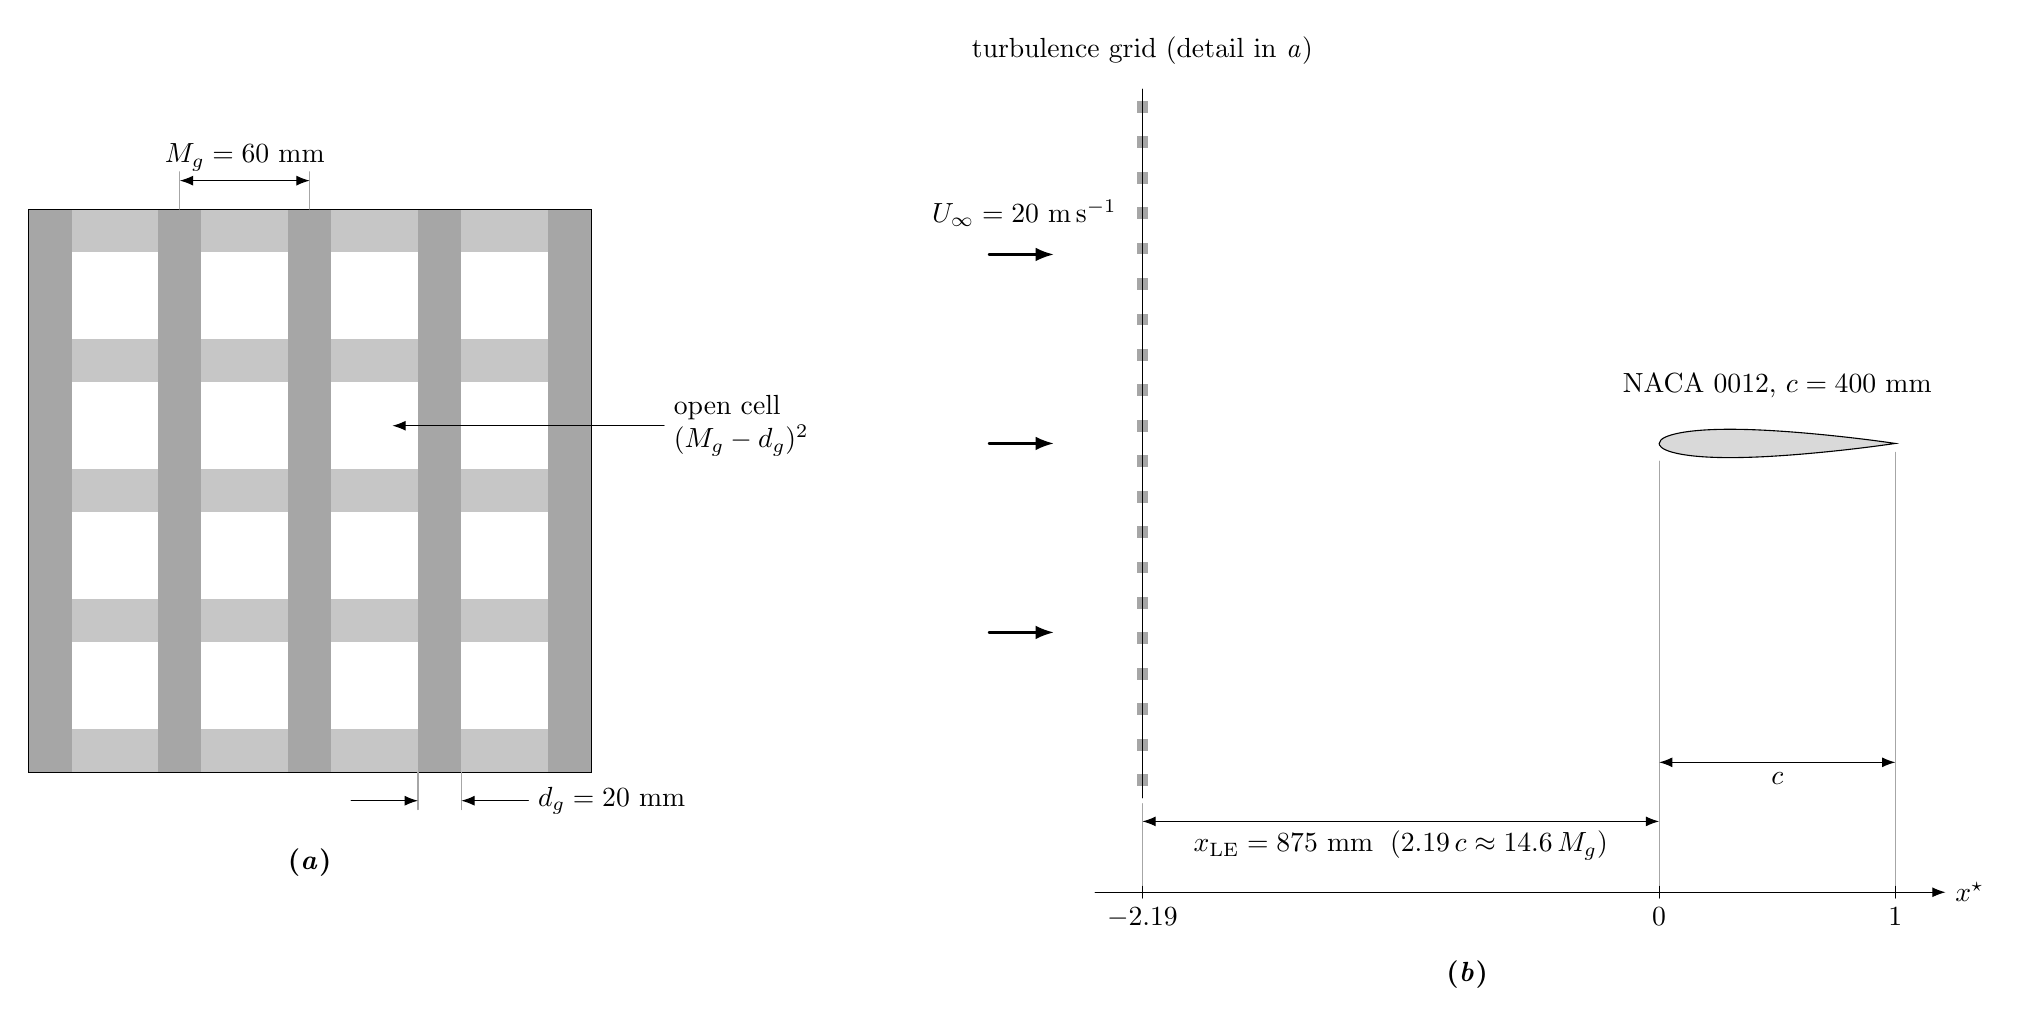
\begin{tikzpicture}[
  >=Latex,
  line cap=round,
  scale=0.75,
  every node/.style={transform shape=false},
  dimline/.style={<->, thin},
  ext/.style={thin,gray!70},
  flow/.style={->, thick},
  lbl/.style={font=\normalsize}
]

%========== (a) Front view of the turbulence grid ==========
\begin{scope}[shift={(0,0)}]
  \def\M{2.2}\def\d{0.7333}\def\N{4}
  \foreach \i in {0,...,\N}{\fill[gray!45] (-0.5*\d, \i*\M-0.5*\d) rectangle (\N*\M+0.5*\d, \i*\M+0.5*\d);}
  \foreach \i in {0,...,\N}{\fill[gray!70] (\i*\M-0.5*\d, -0.5*\d) rectangle (\i*\M+0.5*\d, \N*\M+0.5*\d);}
  \draw[thin] (-0.5*\d,-0.5*\d) rectangle (\N*\M+0.5*\d,\N*\M+0.5*\d);
  \draw[ext] (1*\M, \N*\M+0.5*\d) -- (1*\M, \N*\M+1.0);
  \draw[ext] (2*\M, \N*\M+0.5*\d) -- (2*\M, \N*\M+1.0);
  \draw[dimline] (1*\M, \N*\M+0.85) -- node[above,lbl]{$M_g = 60$~mm} (2*\M, \N*\M+0.85);
  \draw[ext] (3*\M-0.5*\d,-0.5*\d) -- (3*\M-0.5*\d,-1.0);
  \draw[ext] (3*\M+0.5*\d,-0.5*\d) -- (3*\M+0.5*\d,-1.0);
  \draw[<-,thin] (3*\M-0.5*\d,-0.85) -- (3*\M-1.5,-0.85);
  \draw[<-,thin] (3*\M+0.5*\d,-0.85) -- (3*\M+1.5,-0.85) node[right,lbl]{$d_g = 20$~mm};
  \draw[->,thin] (\N*\M+1.6, 2.5*\M) node[right,lbl,align=left]{open cell\\$(M_g-d_g)^2$} -- (2.5*\M+0.3, 2.5*\M);
  \node[lbl] at (0.5*\N*\M,-1.9) {\textbf{(\textit{a})}};
\end{scope}

%========== (b) Computational arrangement, midspan (x,y) plane ==========
% to scale: 1 cm = 100 mm
\begin{scope}[shift={(18.5,5.2)}]
  \def\xLE{8.75}   % 875 mm
  \def\cho{4.0}    % chord 400 mm
  \def\hgrid{6.0}  % grid half-height 600 mm
  % turbulence grid at x = 0 (bars to scale: 20 mm at 60 mm pitch)
  \foreach \yy in {-5.7,-5.1,...,5.7}{\fill[gray!70] (-0.1,\yy-0.1) rectangle (0.1,\yy+0.1);}
  \draw[thin] (0,-\hgrid) -- (0,\hgrid);
  \node[lbl,above,align=center] at (0,\hgrid+0.25) {turbulence grid (detail in \textit{a})};
  % NACA 0012 airfoil at x_LE, to scale (c = 4 cm, t = 0.48 cm)
  \begin{scope}[shift={(\xLE,0)}]
    \draw[fill=gray!30, thin, samples=120, domain=0:1]
      plot ({\cho*\x}, { 5*0.12*\cho*(0.2969*sqrt(\x) - 0.1260*\x - 0.3516*\x*\x + 0.2843*\x*\x*\x - 0.1036*\x*\x*\x*\x)})
      -- plot ({\cho*(1-\x)}, {-5*0.12*\cho*(0.2969*sqrt(1-\x) - 0.1260*(1-\x) - 0.3516*(1-\x)*(1-\x) + 0.2843*(1-\x)*(1-\x)*(1-\x) - 0.1036*(1-\x)*(1-\x)*(1-\x)*(1-\x))})
      -- cycle;
  \end{scope}
  \node[lbl,above] at (\xLE+0.5*\cho,0.6) {NACA 0012, $c = 400$~mm};
  % inflow arrows
  \foreach \yy in {-3.2,0,3.2}{\draw[flow] (-2.6,\yy) -- (-1.5,\yy);}
  \node[lbl,above,align=center] at (-2.0,3.5) {$U_\infty = 20$~m\,s$^{-1}$};
  % dimension chain: grid -> LE, and chord
  \draw[ext] (0,-\hgrid-0.1) -- (0,-7.6);
  \draw[ext] (\xLE,-0.3) -- (\xLE,-7.6);
  \draw[ext] (\xLE+\cho,-0.15) -- (\xLE+\cho,-7.6);
  \draw[dimline] (0,-6.4) -- node[below,lbl]{$x_{\mathrm{LE}} = 875$~mm\; ($2.19\,c \approx 14.6\,M_g$)} (\xLE,-6.4);
  \draw[dimline] (\xLE,-5.4) -- node[below,lbl]{$c$} (\xLE+\cho,-5.4);
  % x* axis
  \draw[->] (-0.8,-7.6) -- (13.6,-7.6) node[right,lbl]{$x^{\star}$};
  \foreach \xx/\tt in {0/-2.19, \xLE/0, 12.75/1}{%
    \draw (\xx,-7.5) -- (\xx,-7.7) node[below,lbl]{$\tt$};}
  \node[lbl] at (5.5,-9.0) {\textbf{(\textit{b})}};
\end{scope}
\end{tikzpicture}
}
\caption{Computational arrangement.
(\textit{a})~Front view of the turbulence grid: square mesh of bars of
width $d_g = 20$~mm at mesh size $M_g = 60$~mm, replicating the AWB
grid (\S\ref{sec:ExpSetup}).
(\textit{b})~Midspan $(x,y)$ view, to scale: the grid plane at
$x^{\star} = -2.19$ and the NACA~0012 airfoil with its leading edge at
$x_{\mathrm{LE}} = 875$~mm downstream --- the station occupied by the
cross-wire probes in the experiment. The wind-tunnel nozzle is not
modelled; grid and airfoil are immersed in a uniform stream of
$U_{\infty} = 20$~m\,s$^{-1}$, with the span $L_z = 800$~mm bounded by
free-slip walls.}
\label{fig:grid_schematic}
\end{figure}

\newpage
% ======================================================================
% COMPUTATIONAL CONFIGURATION -- values extracted from problem.pbu
% (model U20_biggerDomain_likesquareTest, lbpre 3.3.1, 2025/12/09)
% and from the run statistics (pieceDetailedStatistics.txt).
% Remaining flags are marked [CONFIRM]. NO measured turbulence
% quantities appear in this section.
%
% DISCREPANCIES FOUND (do not delete until resolved):
%  1. Re_c: with nu = 1.49e-5 m^2/s from problem.pbu,
%     Re_c = 20*0.4/1.49e-5 = 5.4e5, NOT the 5.1e5 of the conference
%     paper (which implies nu ~ 1.57e-5). The .pbu is authoritative
%     for the simulation; the conference value should be corrected.
%  2. NO nozzle geometry exists in this configuration. Geometries:
%     airfoil, grid, slip-wall box, inlet, outlet, refinement boxes
%     only. Any earlier interpretation of upstream-rms features as a
%     "nozzle-exit signature at x* = -0.95" cannot refer to THIS
%     simulation and must be re-examined (experimental origin? older
%     run?). The results discussion must be made consistent.
%  3. Conference statement "patches one leading-edge radius upstream"
%     is wrong: patches are at x = 0.435/0.460/0.475 m
%     (x* = -1.10/-1.04/-1.00). The nose-conforming toroidal surface
%     approaches to 4 mm = 0.63 r_LE from the LE.
%  4. Legacy artefacts in the .pbu: initial velocity field 30 m/s and
%     run-length normalisation "/30" inherited from the U30 case.
%     Harmless (transient discarded) but worth noting internally.
% ======================================================================

\subsection{Computational configuration and turbulence generation}
\label{sec:method_configuration}

% \begin{figure}
%     \centering
%     \includegraphics[width=0.95\columnwidth]{Figures/grid_schematic.pdf}
%     \caption{Computational arrangement.
%     (\textit{a})~Front view of the turbulence grid: square mesh of
%     bars of width $d_g = 20$~mm at mesh size $M_g = 60$~mm,
%     replicating the AWB grid (\S\ref{sec:ExpSetup}).
%     (\textit{b})~Midspan $(x,y)$ view, to scale: the grid plane at
%     $x^{\star} = -2.19$ and the NACA~0012 airfoil with its leading
%     edge at $x_{\mathrm{LE}} = 875$~mm downstream --- the station
%     occupied by the cross-wire probes in the experiment. The
%     wind-tunnel nozzle is not modelled; grid and airfoil are immersed
%     in a uniform stream of $U_{\infty} = 20$~m\,s$^{-1}$, with the
%     span $L_z = 800$~mm bounded by free-slip walls.}
%     \label{fig:grid_schematic}
% \end{figure}

\subsubsection{Geometry and coordinate system}

The computational arrangement reproduces the turbulence--airfoil
interaction configuration of the AWB experiment
(\S\ref{sec:ExpSetup}): a passive turbulence grid placed upstream of a
NACA~0012 airfoil at zero geometric incidence. A global Cartesian
frame is adopted in which $x$ denotes the streamwise, $y$ the
transverse and $z$ the spanwise direction, with the origin in the
plane of the turbulence grid. The airfoil leading edge lies at
$x_{\mathrm{LE}} = 0.875$~m, i.e.\ $2.19$ chord lengths downstream of
the grid --- the same grid-to-reference-station distance as in the
experiment, where the cross-wire probes occupy this location.
Positions referenced to the airfoil are expressed via
\begin{equation}
  x^{\star} = \frac{x - x_{\mathrm{LE}}}{c},
  \label{eq:xstar_def}
\end{equation}
so that the grid plane corresponds to $x^{\star} = -2.19$ and the
leading and trailing edges to $x^{\star} = 0$ and $x^{\star} = 1$.

The airfoil has chord $c = 0.400$~m and spans the full distance
between the spanwise boundaries, $L_z = 0.800$~m, giving an aspect
ratio $L_z/c = 2$. The maximum thickness is $t = 0.12\,c = 48$~mm and
the geometric leading-edge radius follows from the thickness ratio
$t_c = 0.12$ as
\begin{equation}
  r_{\mathrm{LE}} = 1.1019\,t_c^{2}\,c \approx 6.3~\mathrm{mm}
  \label{eq:rLE_def}
\end{equation}
\citep{AbbottDoenhoff1959}, so that
$r_{\mathrm{LE}}/c = 1.6\times10^{-2}$. The turbulence grid replicates
the experimental geometry of \S\ref{sec:ExpSetup}, with bar width
$d_g = 20$~mm and mesh size $M_g = 60$~mm.
% [CONFIRM: STL "Grid_NACA0012_ascii - Part1-2" -- verify the bar
%  cross-section and pitch in the STL match the experimental
%  d_g = 20 mm, M_g = 60 mm]
The grid-to-leading-edge separation thus corresponds to
$x_{\mathrm{LE}}/M_g \approx 14.6$ mesh sizes, beyond the conventional
minimum of about $10\,M_g$ for the bar wakes to merge into a
spatially decorrelated field \citep{Roach1987,ComteBellotCorrsin1971},
yet short enough that the energy-containing scales remain energetic
on arrival. The wind-tunnel nozzle is not modelled: grid and airfoil
are immersed in a single free domain, so that the incident turbulence
develops in a nominally uniform stream rather than within the
experimental contraction and jet.

\subsubsection{Non-dimensional parameters and characteristic scales}

The leading-edge radius constitutes the geometric inner scale of the
interaction and enters the analysis through the dimensionless
wavenumber
\begin{equation}
  \kappa = k\,r_{\mathrm{LE}},
  \label{eq:kappa_def}
\end{equation}
which compares the scale of an incident turbulent structure with the
scale of the nose geometry it encounters; the chord-based Strouhal
number $St_c = fc/U_{\infty}$ provides the complementary outer-scale
frequency parameter. Throughout this paper $\kappa$ is reserved
exclusively for $k\,r_{\mathrm{LE}}$; streamwise distances scaled by
the nose radius are written $x/r_{\mathrm{LE}}$, and the azimuthal
coordinate on the nose-conforming sampling surfaces is denoted
$\phi$.

The free-stream velocity is $U_{\infty} = 20$~m\,s$^{-1}$. With the
reference sound speed $c_0 = 343.2$~m\,s$^{-1}$ and kinematic
viscosity $\nu = 1.49\times10^{-5}$~m$^2$\,s$^{-1}$ (air at
$p_0 = 101\,325$~Pa, $T_0 = 293.15$~K, $\rho_0 = 1.204$~kg\,m$^{-3}$),
the Mach number is $M = 0.058$ and the chord-based Reynolds number
$Re_c = U_{\infty}c/\nu \approx 5.4\times10^{5}$.
% [NOTE: the conference paper states 5.1e5; the problem definition
%  gives nu = 1.49e-5, hence 5.4e5. Correct the published value or
%  identify the nu used there.]
At this Mach number the flow is effectively incompressible at the
level of the turbulence dynamics, while the compressible
lattice-Boltzmann formulation (\S\ref{sec:numerical}) retains the
acoustic degrees of freedom.

Two kinematic scales follow directly from the configuration and
parameterise the theoretical framework of \S\ref{sec:3}. An ideal
stagnation flow about a nose of radius $r_{\mathrm{LE}}$ possesses
the strain-rate scale
\begin{equation}
  a \sim \frac{U_{\infty}}{2\,r_{\mathrm{LE}}}
    \approx 1.6\times10^{3}~\mathrm{s}^{-1},
  \label{eq:strain_scale}
\end{equation}
and the convection time across one nose radius is
$\tau \sim r_{\mathrm{LE}}/U_{\infty} \approx 3.2\times10^{-4}$~s, so
that the a~priori estimate of the integrated distortion parameter is
\begin{equation}
  \vartheta = a\tau = \mathcal{O}(1/2).
  \label{eq:vartheta_estimate}
\end{equation}
These are geometric estimates, independent of the turbulence realised
in the computation; the strain field actually established in the
stagnation region is assessed from the data in \S\ref{sec:results}.

\subsubsection{Computational domain and boundary conditions}

The domain is a rectangular box extending from $x = -6.0$~m to
$x = +8.96$~m in the streamwise direction
($x^{\star} \in [-17.2,\,+20.2]$), $16.6$~m in the transverse
direction and $0.928$~m in the spanwise direction. A uniform velocity
inlet ($U_{\infty} = 20$~m\,s$^{-1}$) is imposed on a face at
$x \approx -5.7$~m, $14.3\,c$ upstream of the turbulence grid, and a
static-pressure outlet ($p_0 = 101\,325$~Pa) at $x \approx +8.7$~m,
$18.6\,c$ downstream of the trailing edge. The large streamwise
margins ensure that the imposed uniform inflow does not constrain the
development of the grid wakes and that the airfoil wake leaves the
region of interest without upstream contamination.

In the spanwise direction the flow is bounded by a pair of
frictionless (free-slip) walls separated by $L_z = 0.800$~m, between
which the airfoil spans wall to wall; the geometry is thus nominally
homogeneous in $z$ without enforcing spanwise periodicity. The same
free-slip box bounds the domain transversely at approximately
$\pm 8$~m ($\pm 20\,c$) from the model, giving a geometric blockage
of the airfoil section below $0.3\,\%$. All inlet, outlet and
free-slip boundaries are backed by absorbing (sponge) layers of
$0.3$~m thickness, in which the fluctuating fields are progressively
relaxed toward the corresponding far-field state; this treatment
suppresses the spurious reflection of hydrodynamic and acoustic
disturbances, the latter being of particular concern for a
compressible time-domain method in which outgoing waves are
explicitly resolved.

\subsubsection{Spatial resolution}

The lattice is block-refined over nine refinement levels with a
factor of two between successive levels, spanning lattice spacings
from $\Delta x_{\min} = 0.5$~mm to $128$~mm. The finest level is
concentrated at the airfoil surface and in a trailing-edge box, so
that the nose radius is covered by
$r_{\mathrm{LE}}/\Delta x_{\min} = 12.6$ cells and the chord by $800$
cells. The turbulence grid, and the entire corridor connecting it to
the airfoil, are resolved with $\Delta x = 4$~mm, corresponding to
five cells across each grid bar and approximately ten cells per
wavelength at the geometric crossover scale
$\lambda(\kappa{=}1) = 2\pi r_{\mathrm{LE}} \approx 40$~mm; the same
wavelength is covered by about $80$ cells in the near-nose region
where the distortion is interrogated. Intermediate boxes at $2$~mm
(near wake) and $16$~mm, embedded in a $128$~mm background, complete
the hierarchy. The complete mesh comprises $557\times10^{6}$ fluid
nodes, of which $41\,\%$ lie on the finest level; the fine-equivalent
update count is $2.8\times10^{8}$ nodes. At solid surfaces a
wall-function boundary treatment is applied
(\S\ref{sec:numerical}), and the subgrid stresses are closed with the
shear-improved Smagorinsky model \citep{Leveque2007}.

\subsubsection{Time advancement, statistical sampling and record
length}

The time step at the finest level is fixed by the acoustic lattice
condition $\Delta t = \Delta x_{\min}/(\sqrt{3}\,c_0)
= 8.41\times10^{-7}$~s. The simulation is advanced for
$792\,596$ fine-level steps, i.e.\ a physical time of $0.667$~s
corresponding to $33.3$ flow-through times $c/U_{\infty} = 0.02$~s.
The first half of the run ($0.333$~s, equal to $16.7\,c/U_{\infty}$
or $7.6$ grid-to-leading-edge convection times) is discarded as the
initial transient; all statistics are accumulated over the remaining
$0.333$~s. Statistical stationarity of the retained record is
verified by comparison of statistics over its first and second
halves, reported alongside the corresponding quantities in
\S\ref{sec:results}.
% [CONFIRM: recording periods are interpreted in fine-level steps;
%  verify against output time stamps]

Three families of recording locations are employed
(\S\ref{sec:sampling} gives their geometric construction).
(i)~A midspan probe line of $200$ stations spanning
$x \in [0,\,2.075]$~m at $10.4$~mm spacing --- from the grid plane to
$2\,c$ behind the trailing edge --- records velocity and pressure at
$23.8$~kHz; on it, mean profiles, Reynolds stresses and anisotropy
invariants are evaluated as functions of $x^{\star}$.
(ii)~Three planar patches of $32\times32$ points at
$x = 0.435$, $0.460$ and $0.475$~m
($x^{\star} = -1.10$, $-1.04$, $-1.00$), each spanning $1.2$~m
transversely and the full $0.8$~m span, are sampled at $5.94$~kHz;
they establish the upstream reference state
$\Phi^{\infty}_{ij}$ and, through their mutual streamwise
separations, permit an estimate of the convection velocity from
cross-spectral phase.
(iii)~A geometry-matched pair of nose-conforming surfaces of
identical topology and point count ($1000$ points each, $25$ spanwise
stations), sampled at $5.94$~kHz: one wraps the leading edge from
$4$~mm ($0.63\,r_{\mathrm{LE}}$) ahead of the nose to
$x^{\star} = 0.25$, and its upstream twin occupies
$x \in [0.746,\,0.850]$~m, terminating $4\,r_{\mathrm{LE}}$ ahead of
the leading edge. The Nyquist frequency of the patch records
($2.97$~kHz) lies far above the frequency band in which
$\kappa = \mathcal{O}(1)$ is anticipated for any plausible convection
velocity, so the geometric crossover region is bracketed with margin.
All spectral estimates employ a frequency resolution
$\Delta f = U_{\infty}/(10c) = 5$~Hz, resolving the range
$St_c \in [0.1,\,200]$; the estimation procedure, patch aggregation
and reliability thresholds are given in \S\ref{sec:methodology_gain}.

\begin{table}
  \begin{center}
  \def~{\hphantom{0}}
  \begin{tabular}{lll}
    Quantity & Symbol & Value \\[3pt]
    Airfoil section                  & ---                & NACA~0012, zero incidence \\
    Chord                            & $c$                & $0.400$~m \\
    Span (slip-wall to slip-wall)    & $L_z$              & $0.800$~m \quad ($L_z/c = 2$) \\
    Leading-edge radius              & $r_{\mathrm{LE}}$  & $6.3$~mm \quad ($r_{\mathrm{LE}}/c = 1.6\times10^{-2}$) \\
    Grid--leading-edge separation    & $x_{\mathrm{LE}}$  & $0.875$~m \quad ($2.19\,c = 14.6\,M_g$) \\
    Grid bar width / mesh size       & $d_g$ / $M_g$      & $20$~mm / $60$~mm \\
    Free-stream velocity             & $U_{\infty}$       & $20$~m\,s$^{-1}$ \\
    Mach number                      & $M$                & $0.058$ \\
    Chord Reynolds number            & $Re_c$             & $5.4\times10^{5}$ \\
    Stagnation strain-rate scale     & $a$                & $\approx 1.6\times10^{3}$~s$^{-1}$ (Eq.~\ref{eq:strain_scale}) \\
    Distortion parameter (estimate)  & $\vartheta$        & $\mathcal{O}(1/2)$ (Eq.~\ref{eq:vartheta_estimate}) \\
    Finest lattice spacing           & $\Delta x_{\min}$  & $0.5$~mm \quad ($r_{\mathrm{LE}}/\Delta x_{\min} = 12.6$) \\
    Grid-corridor lattice spacing    & ---                & $4$~mm \quad ($\approx 10$ cells per $\lambda(\kappa{=}1)$) \\
    Refinement levels                & ---                & $9$ \quad ($\Delta x$: $0.5$--$128$~mm) \\
    Fluid nodes                      & ---                & $557\times10^{6}$ \\
    Fine time step                   & $\Delta t$         & $8.41\times10^{-7}$~s \\
    Total run / retained record      & ---                & $33.3$ / $16.7$ $\times\,c/U_{\infty}$ \\
    Sampling rates (line / patches)  & ---                & $23.8$ / $5.94$~kHz \\
    Frequency resolution             & $\Delta f$         & $5$~Hz \quad ($St_c \in [0.1,\,200]$) \\
  \end{tabular}
  \caption{Summary of the computational configuration (problem
  definition U20, ProLB~3.3.1).}
  \label{tab:config}
  \end{center}
\end{table}

\bibliographystyle{jfm}
\bibliography{jfm}

\end{document}

% =========================================================================
% Section 2 — Theoretical framework: pre-impact distortion as a tensorial
% mapping. Target: Journal of Fluid Mechanics (natbib, \citep / \citet).
%
% NOTATION DECISIONS (must propagate through the manuscript):
%   - \vartheta : integrated-strain (distortion) parameter, formerly θ in
%                 the conference §II. Resolves the collision with the
%                 azimuthal coordinate.
%   - \theta    : azimuthal coordinate around the leading edge, in the
%                 MIDSPAN (x,y) plane, θ = 0 on the upstream stagnation
%                 line (PDF Fig. 4 convention).
%   - Local cylindrical projection acts on (u,v) in the midspan plane,
%     with w unchanged (PDF Eq. 27 convention). >>> DECISION POINT: if the
%     post-processing in fact projected (v,w) in the (y,z) plane, §2.6
%     and the trace identity (eq:trace) must be changed accordingly. <<<
% =========================================================================

\section{Theoretical framework: pre-impact distortion as a tensorial mapping}
\label{sec:framework}

\subsection{Flow configuration and the two turbulence states}
\label{sec:framework_states}

We consider statistically stationary turbulence, generated far upstream and
carried by a uniform mean stream $U_\infty \boldsymbol{e}_x$, convecting onto
a symmetric airfoil of chord $c$ and leading-edge radius $r_{\mathrm{LE}}$
held at zero incidence. Cartesian coordinates $(x,y,z)$ denote the
streamwise, transverse and spanwise directions, with the origin such that
the leading edge lies at $x = x_{\mathrm{LE}}$, $y = 0$. The configuration
is statistically homogeneous in $z$ and stationary in time, and the
turbulence intensity is small, $u'_\infty/U_\infty \ll 1$, so that the mean
flow may be treated as the steady flow past the airfoil, unmodified at
leading order by the fluctuations.

The analysis is organised around two turbulence states, defined as
statistical ensembles on two control surfaces rather than by reference to
any particular measurement apparatus. The \emph{upstream state} is the
ensemble of velocity and pressure fluctuations on a plane
$\mathcal{S}_\infty$ normal to $\boldsymbol{e}_x$, located a distance
$\ell_\infty$ ahead of the leading edge, with $\ell_\infty$ chosen large
enough that the mean flow on $\mathcal{S}_\infty$ is uniform to within a
prescribed tolerance, yet small enough that free decay between
$\mathcal{S}_\infty$ and the airfoil is negligible compared with the
distortion to be quantified. The \emph{pre-impact state} is the ensemble on
a surface $\mathcal{S}_{\mathrm{LE}}$ conformal to the airfoil nose,
displaced from the wall by a fixed offset small compared with
$r_{\mathrm{LE}}$, on which the fluctuations have traversed the
stagnation-region mean strain but have not yet participated in the
scattering that produces the acoustic field. The acoustic response itself
is outside the scope of this framework: we characterise the transformation
of the turbulence between $\mathcal{S}_\infty$ and
$\mathcal{S}_{\mathrm{LE}}$, which precedes and conditions the scattering
problem treated by classical theory \citep{Amiet1975,Goldstein1976}.

Two local frames are attached to $\mathcal{S}_{\mathrm{LE}}$. Because the
nose is locally cylindrical, points on $\mathcal{S}_{\mathrm{LE}}$ in the
midspan plane are parametrised by the azimuthal angle $\theta$ measured
about the centre of the osculating nose circle, with $\theta = 0$ on the
upstream stagnation line and $\theta \gtrless 0$ on the two sides of the
airfoil. The associated cylindrical unit vectors are
$\boldsymbol{e}_r(\theta)$ and $\boldsymbol{e}_\theta(\theta)$, lying in
the $(x,y)$ plane, together with $\boldsymbol{e}_z$. On the nose circle the
surface-aligned frame $(t,n,z)$ coincides with this cylindrical frame,
$\boldsymbol{e}_n = \boldsymbol{e}_r$ and
$\boldsymbol{e}_t = \boldsymbol{e}_\theta$, so that `wall-normal' and
`radial' are used interchangeably there; away from the nose circle the two
frames separate and the distinction must be retained. All azimuthally
resolved quantities below are referred to this frame.

In this frame, the mean rate of strain experienced by fluid approaching and
rounding the nose takes, near the surface, the approximate form
\begin{equation}
  \mathsf{S} \;\approx\; a\,(\boldsymbol{e}_t\boldsymbol{e}_t
                            - \boldsymbol{e}_n\boldsymbol{e}_n),
  \qquad a > 0,
  \label{eq:strain_local}
\end{equation}
i.e. extension along the surface tangent and compression along the surface
normal, with the spanwise direction neutral. We emphasise that
(\ref{eq:strain_local}) is written in the \emph{local surface frame}: on
the upstream stagnation streamline, where
$\boldsymbol{e}_n = -\boldsymbol{e}_x$, the same tensor corresponds to
streamwise compression ($\partial \overline{U}/\partial x < 0$ as the flow
decelerates toward the stagnation point) and transverse extension. This is
the canonical plane stagnation flow of rapid distortion theory
\citep{BatchelorProudman1954,Hunt1973}, and it is the agent of the
transformation studied here.

\subsection{Spectral and single-point statistical descriptions}
\label{sec:framework_descriptions}

Let $\boldsymbol{u}'(\boldsymbol{x},t)$ and $p'(\boldsymbol{x},t)$ denote
the velocity and pressure fluctuations about the mean. The two-point,
two-time correlation tensor is
\begin{equation}
  R_{ij}(\boldsymbol{x};\boldsymbol{r},\tau)
  = \big\langle u_i'(\boldsymbol{x},t)\,
                u_j'(\boldsymbol{x}+\boldsymbol{r},\,t+\tau) \big\rangle ,
  \label{eq:twopoint}
\end{equation}
where $\langle\cdot\rangle$ denotes the ensemble (here, time and spanwise)
average. Where the turbulence may be treated as locally homogeneous and
stationary, the wavenumber--frequency spectral tensor is the Fourier
transform of (\ref{eq:twopoint}),
\begin{equation}
  \Phi_{ij}(\boldsymbol{k},\omega)
  = \frac{1}{(2\pi)^4}
    \int\!\!\int R_{ij}(\boldsymbol{r},\tau)\,
    \mathrm{e}^{-\mathrm{i}(\boldsymbol{k}\cdot\boldsymbol{r}-\omega\tau)}
    \,\mathrm{d}\boldsymbol{r}\,\mathrm{d}\tau ,
  \qquad
  \int\!\!\int \Phi_{ij}\,\mathrm{d}\boldsymbol{k}\,\mathrm{d}\omega
  = \big\langle u_i' u_j' \big\rangle ,
  \label{eq:spectraltensor}
\end{equation}
which is Hermitian and positive semi-definite at every
$(\boldsymbol{k},\omega)$ \citep{Batchelor1953,Pope2000}. The flow at hand
is inhomogeneous in $x$ and $y$; the directions of exact statistical
symmetry are $z$ and $t$. Accordingly, the quantities that are defined
without approximation at every point are the one-sided frequency spectra
\begin{equation}
  \int_0^\infty \Phi_{qq}(f)\,\mathrm{d}f = \big\langle q'^2 \big\rangle ,
  \qquad q \in \{u, v, w, p\},
  \label{eq:freqspec}
\end{equation}
together with the corresponding cross-spectra, and the superscripts
$\infty$ and $\mathrm{LE}$ will indicate evaluation on
$\mathcal{S}_\infty$ and $\mathcal{S}_{\mathrm{LE}}$ respectively. The
passage from frequency to wavenumber, which is required to compare the
data with wavenumber-space theory, is an additional modelling step and is
treated separately in \S\,\ref{sec:framework_observables}.

The single-point state is summarised by the Reynolds-stress tensor
$R_{ij} = \langle u_i' u_j' \rangle$, the kinetic energy
$k = \tfrac{1}{2}R_{ii}$, and the anisotropy tensor
\begin{equation}
  b_{ij} = \frac{R_{ij}}{2k} - \frac{1}{3}\delta_{ij},
  \qquad
  II = -\tfrac{1}{2}\,b_{ij}b_{ji},
  \qquad
  III = \tfrac{1}{3}\,b_{ij}b_{jk}b_{ki},
  \label{eq:anisotropy}
\end{equation}
whose invariants $(III,-II)$ locate the state within the realisable region
bounded by the axisymmetric and two-component limits
\citep{LumleyNewman1977,Banerjee2007}. We stress that $(III,-II)$ is a
\emph{state} space: a trajectory traced in it by sampling successive
streamwise stations records the structural evolution of the stress tensor,
normalised free of amplitude, and is logically distinct from any trajectory
in physical space. The spectral description (\ref{eq:spectraltensor})
resolves the transformation by scale; the invariant description
(\ref{eq:anisotropy}) resolves it by tensorial structure. Both are needed,
because a mapping may preserve single-point invariants while redistributing
energy across scales, and conversely.

\subsection{The distortion-operator hypothesis}
\label{sec:framework_hypothesis}

The central proposition of this paper --- a proposed formulation, not an
established result --- is that the action of the leading-edge mean flow on
the incident turbulence is usefully represented as a linear mapping between
the two spectral tensors,
\begin{equation}
  \Phi^{\mathrm{LE}}_{ij}(\boldsymbol{k},\omega;\theta)
  = \mathcal{D}_{ijmn}(\boldsymbol{k},\vartheta;\theta)\,
    \Phi^{\infty}_{mn}(\boldsymbol{k},\omega),
  \label{eq:operator}
\end{equation}
in which $\mathcal{D}_{ijmn}$ is a dimensionless fourth-order operator,
$\vartheta$ is the integrated-strain parameter defined in
\S\,\ref{sec:framework_groups}, and the dependence on the azimuthal station
$\theta$ records the fact that the pre-impact state is inhomogeneous along
$\mathcal{S}_{\mathrm{LE}}$. Summation over repeated indices is implied.
Since $\Phi^{\infty}$ and $\Phi^{\mathrm{LE}}$ share dimensions,
$\mathcal{D}$ is dimensionless; and since both tensors must be Hermitian
and positive semi-definite, $\mathcal{D}$ is constrained to map the cone of
realisable spectral tensors into itself. These are structural requirements
on any admissible $\mathcal{D}$, not properties we claim to have verified
componentwise.

The hypothesis rests on assumptions that we state explicitly.
\emph{(i) Stationarity}: both states are statistically stationary, so that
the mapping is time-independent. \emph{(ii) Linearity in
$\Phi^{\infty}$}: the transformation of each spectral component is taken to
be independent of the amplitude of the others. This is the rapid-distortion
approximation, formally justified when the transit time
$\tau_{\mathrm{t}}$ of a fluid parcel from $\mathcal{S}_\infty$ to
$\mathcal{S}_{\mathrm{LE}}$ is short compared with the eddy turnover time
$L_\infty/u'_\infty$ of the energy-containing scales, so that the
mean-strain term dominates the nonlinear interactions in the fluctuation
equations \citep{BatchelorProudman1954,HuntCarruthers1990}.
\emph{(iii) Frozen mean geometry}: the mean flow is steady and is the sole
agent of the transformation; free decay over the transit is neglected, an
approximation controlled by the same time-scale separation.
Assumption~(ii) is a modelling assumption whose breakdown is itself of
interest: the diagnostics of \S\,\ref{sec:framework_observables} are
constructed so that signatures of nonlinear, finite-time effects ---
in particular pressure--strain redistribution
\citep{SpezialeSarkarGatski1991} --- appear as identifiable departures from
the linear predictions, rather than being absorbed invisibly.

Equation~(\ref{eq:operator}) deliberately relocates the modelling burden.
In Amiet-type formulations the incident spectrum is prescribed and the
entire interaction is carried by an aerodynamic--acoustic transfer
function \citep{Amiet1975}; corrections for finite thickness then enter as
modifications of that transfer function or as fitted attenuation factors.
Here the transfer function is left untouched and the modification is
assigned to the turbulence itself, following the precedent of
rapid-distortion corrections to the incident upwash spectrum
\citep{deSantana2016} but generalised from a corrected scalar spectrum to a
mapping of the full tensor. We do not claim that
(\ref{eq:operator}) constitutes a closure: $\mathcal{D}$ is introduced as
an organising and diagnostic framework, to be constrained empirically, and
the limits of its identifiability from the present data are stated in
\S\,\ref{sec:framework_observables}.

\subsection{Linear rapid-distortion structure: straining and blocking}
\label{sec:framework_rdt}

Linear theory supplies the expected structure of $\mathcal{D}$, and ---
importantly for the interpretation of the results --- it supplies
\emph{two} physically distinct contributions of opposite tendency for the
wall-normal component.

The first is distortion by the mean strain. For weak turbulence carried
through a spatially smooth mean flow, each Fourier mode evolves
independently along mean trajectories \citep{BatchelorProudman1954}.
Conservation of phase under the local deformation gradient
$\mathsf{F}(\vartheta)$ of the mean flow implies that an upstream mode of
wavevector $\boldsymbol{k}_0$ arrives with wavevector
\begin{equation}
  \boldsymbol{k} = \mathsf{F}^{-\top}(\vartheta)\,\boldsymbol{k}_0,
  \qquad\text{equivalently}\qquad
  \boldsymbol{k}_0 = \mathsf{F}^{\top}(\vartheta)\,\boldsymbol{k},
  \label{eq:kvec}
\end{equation}
so that spectral support is redistributed in wavenumber space, while
incompressibility, $\nabla\cdot\boldsymbol{u}' = 0$, is enforced mode by
mode through the solenoidal projector
\begin{equation}
  \Pi_{ij}(\boldsymbol{k}) = \delta_{ij}
  - \frac{k_i k_j}{\|\boldsymbol{k}\|^{2}} .
  \label{eq:projector}
\end{equation}
The strain contribution to the operator therefore has the structural form
\begin{equation}
  \mathcal{D}(\boldsymbol{k},\vartheta)\big[\Phi^{\infty}\big]
  \;\sim\;
  \Pi(\boldsymbol{k})\,\mathsf{F}(\vartheta)\,
  \Phi^{\infty}\!\big(\mathsf{F}^{\top}(\vartheta)\boldsymbol{k},\,\omega\big)\,
  \mathsf{F}^{\top}(\vartheta)\,\Pi(\boldsymbol{k}),
  \label{eq:rdt_structure}
\end{equation}
which we use throughout as a structural guide --- it fixes which couplings
between components and wavevectors are admissible at linear order --- and
not as a closed predictive model.

The second contribution is the inviscid blocking imposed by the
impermeable surface. Following \citet{Hunt1973}, the fluctuation field near
a bluff body may be decomposed into the strained free-stream part and an
irrotational correction $\boldsymbol{u}^{(s)} = \nabla\phi^{(s)}$, with
$\phi^{(s)}$ harmonic and chosen so that the total normal velocity vanishes
on the surface,
\begin{equation}
  \frac{\partial \phi^{(s)}}{\partial n}\bigg|_{\mathrm{wall}}
  = -\,\boldsymbol{u}^{(d)}\!\cdot\boldsymbol{n},
  \label{eq:blocking}
\end{equation}
where $\boldsymbol{u}^{(d)}$ is the strained (distorted) free-stream
contribution. The blocking correction decays away from the surface over a
distance comparable to the eddy length scale, so that eddies large compared
with the body scale are modified throughout the region they occupy, whereas
small eddies are affected only within a thin layer
\citep{Hunt1973,HuntGraham1978}. Its principal effect is to suppress the
surface-normal velocity component at the expense of a redistribution into
the tangential components.

The two mechanisms compete. For the plane strain
(\ref{eq:strain_local}), free-space rapid distortion tends to amplify the
fluctuation component aligned with the compressive (here surface-normal)
principal axis, whereas blocking suppresses precisely that component near
the wall. For a circular cylinder of radius $a_{\mathrm{cyl}}$,
\citet{Hunt1973} showed, and \citet{Bearman1972} and
\citet{BritterHuntMumford1979} confirmed experimentally, that the outcome
on the stagnation line is organised by the ratio of eddy size to body
radius: the variance of the body-normal component of eddies large compared
with $a_{\mathrm{cyl}}$ is reduced on approach (blocking-dominated), while
sufficiently small-scale content is amplified by the straining. The
transposition of this competition to an airfoil nose, with the leading-edge
radius $r_{\mathrm{LE}}$ playing the role of the body scale, is a
hypothesis of the present work; it is consistent with, but not established
by, the documented sensitivity of high-frequency leading-edge noise to nose
geometry \citep{Gill2013,DevenportStaubsGlegg2010} and with
rapid-distortion corrections applied to measured upwash spectra
\citep{deSantana2016,dosSantos2023}. Verifying it, and locating the
crossover, is one task of the diagnostics defined below.

\subsection{Dimensionless groups and limiting regimes}
\label{sec:framework_groups}

Two dimensionless groups govern the linear problem. The first compares the
turbulent scale with the geometric scale of the nose,
\begin{equation}
  \kappa = k\, r_{\mathrm{LE}},
  \label{eq:kappa}
\end{equation}
where $k = \|\boldsymbol{k}\|$. The second measures the total strain
accumulated along a mean trajectory $\boldsymbol{X}(t')$ from
$\mathcal{S}_\infty$ to the station $\theta$ on
$\mathcal{S}_{\mathrm{LE}}$,
\begin{equation}
  \vartheta(\theta) = \int_{0}^{\tau_{\mathrm{t}}}
  a\big(\boldsymbol{X}(t')\big)\,\mathrm{d}t' ,
  \label{eq:vartheta}
\end{equation}
with $a$ the local principal strain rate of (\ref{eq:strain_local}) and
$\tau_{\mathrm{t}}$ the transit time. An elementary potential-flow estimate
fixes the magnitude of $a$ near the nose: for irrotational flow past a
circular cylinder of radius $r_{\mathrm{LE}}$, the tangential strain rate
at the stagnation point is $2U_\infty/r_{\mathrm{LE}}$, so that
$a = \mathcal{O}(U_\infty/r_{\mathrm{LE}})$ in the pre-impact region, and
the strain is concentrated within a region of extent
$\mathcal{O}(r_{\mathrm{LE}})$ around the nose.

The operator structure of \S\,\ref{sec:framework_rdt} then implies two
limiting regimes, which we state as expectations to be tested rather than
as established results for this geometry:
\begin{equation}
  \kappa \lesssim 1:\;\;
  \mathcal{D} \text{ far from identity, blocking-dominated for the normal
  component};
  \qquad
  \kappa \gg 1:\;\;
  \mathcal{D} \to \mathcal{I},
  \label{eq:limits}
\end{equation}
where $\mathcal{I}_{ijmn} = \delta_{im}\delta_{jn}$. The first limit
follows from the blocking analysis: eddies with wavelengths exceeding
$r_{\mathrm{LE}}$ cannot satisfy impermeability without a substantial
irrotational correction, and their surface-normal content is suppressed
over the whole pre-impact region. The second limit reflects two compounding
facts: the blocking layer for small eddies is thin compared with the
sampling offset, and the strain accumulated over the short residence of a
small, rapidly convected eddy within the $\mathcal{O}(r_{\mathrm{LE}})$
strain region is small. The crossover is therefore expected at
$\kappa = \mathcal{O}(1)$, which identifies $r_{\mathrm{LE}}$ as the
geometric filter scale separating strongly and weakly distorted classes of
motion. We note for later reference that the validity of the linear
framework is itself scale-dependent: the rapid-distortion condition is most
secure for the large, slowly evolving scales and degrades as the eddy
turnover time decreases, so that the $\kappa \gg 1$ limit is approached for
reasons partly outside linear theory.

\subsection{Observable projections, frequency--wavenumber assignment, and
identifiability}
\label{sec:framework_observables}

The data to be presented are pointwise frequency spectra and cross-plane
statistics on the two surfaces. The diagnostics are therefore defined now,
as projections of $\mathcal{D}$, so that the results sections evaluate
pre-declared quantities.

The primary diagnostic is the component-wise spectral gain
\begin{equation}
  G_q(f) = \frac{\Phi^{\mathrm{LE}}_{qq}(f)}{\Phi^{\infty}_{qq}(f)},
  \qquad q \in \{u,v,w,p\},
  \label{eq:gain}
\end{equation}
the ratio of like-component power spectral densities, with no implied
summation over $q$. Departures of $G_q$ from unity measure the amplitude
of the transformation at each scale; inequality among the $G_q$ at fixed
$f$ is the signature that the mapping is tensorial, i.e. not expressible
as $\Phi^{\mathrm{LE}} = \alpha(f)\,\Phi^{\infty}$ for any scalar
$\alpha$. Because (\ref{eq:gain}) is a ratio of power spectral densities,
any acoustic quantity linear in the incident spectrum --- such as the
far-field pressure spectral density of Amiet-type models, which is
proportional to the upwash spectrum \citep{Amiet1975} --- inherits the
factor $G$ linearly, not quadratically.

Azimuthal structure is resolved by projecting the midspan-plane velocity
components onto the cylindrical frame of
\S\,\ref{sec:framework_states},
\begin{equation}
  u_r = u\cos\theta + v\sin\theta,
  \qquad
  u_\theta = -\,u\sin\theta + v\cos\theta,
  \qquad
  u_z = w,
  \label{eq:projection}
\end{equation}
an orthogonal rotation in the $(x,y)$ plane, which preserves the in-plane
trace,
\begin{equation}
  \Phi_{uu} + \Phi_{vv} = \Phi_{rr} + \Phi_{\theta\theta},
  \qquad
  \Phi_{zz} = \Phi_{ww},
  \label{eq:trace}
\end{equation}
so that any inequality between $\Phi_{rr}$ and $\Phi_{\theta\theta}$
reflects genuine directional redistribution rather than an artefact of the
frame. The azimuthally resolved distortion is quantified by
\begin{equation}
  \Delta_{qq}(St_c,\theta)
  = \log_{10}
    \frac{\widetilde{\Phi}^{\mathrm{LE}}_{qq}(St_c,\theta)}
         {\widetilde{\Phi}^{\infty}_{qq}(St_c,\theta)},
  \qquad q \in \{r,\theta\},
  \qquad
  \widetilde{\Phi}_{qq} = St_c\,\Phi_{qq},
  \label{eq:delta}
\end{equation}
with $St_c = fc/U_\infty$, together with two reduced quantities: the
in-plane trace gain
\begin{equation}
  G_\perp(St_c,\theta)
  = \frac{\widetilde{\Phi}^{\mathrm{LE}}_{rr}
        + \widetilde{\Phi}^{\mathrm{LE}}_{\theta\theta}}
         {\widetilde{\Phi}^{\infty}_{rr}
        + \widetilde{\Phi}^{\infty}_{\theta\theta}},
  \label{eq:tracegain}
\end{equation}
which by (\ref{eq:trace}) is invariant under rotations in the projection
plane and isolates the net in-plane energy change, and the in-plane
anisotropy parameter
\begin{equation}
  \chi = \frac{\Phi_{rr} - \Phi_{\theta\theta}}
              {\Phi_{rr} + \Phi_{\theta\theta}},
  \qquad
  \Delta\chi = \chi^{\mathrm{LE}} - \chi^{\infty},
  \label{eq:chi}
\end{equation}
which isolates directional redistribution independently of energy level.
The single-point counterpart of these scale-resolved diagnostics is the
trajectory of $(III,-II)$ of (\ref{eq:anisotropy}) along the approach,
which records the structural transformation integrated over all scales.

Comparison with the wavenumber-space theory of
\S\S\,\ref{sec:framework_rdt}--\ref{sec:framework_groups} requires
assigning a wavenumber to each measured frequency. We adopt the
frozen-convection assignment
\begin{equation}
  \kappa(f) = \frac{2\pi f\, r_{\mathrm{LE}}}{U_c(f)},
  \label{eq:kappa_f}
\end{equation}
where $U_c(f)$ is the convection velocity estimated from the phase of
streamwise cross-spectra between adjacent upstream probes. This step
carries known caveats, which we state as limitations rather than resolve:
the hypothesis of frozen convection \citep{Taylor1938} is least secure
precisely where the distortion is strongest, since the mean flow
decelerates and the convection velocity is scale-dependent in
inhomogeneous turbulence
\citep{WyngaardClifford1977,DelAlamoJimenez2009}. Accordingly,
(\ref{eq:kappa_f}) is applied with $U_c$ evaluated on the upstream side,
$\kappa$ values quoted near the leading edge are interpreted as nominal,
and no conclusion below rests on the precise location of the
$\kappa = \mathcal{O}(1)$ crossover, only on its existence and on the
component ordering across it. With $U_c \approx U_\infty$,
(\ref{eq:kappa_f}) places $\kappa = 1$ at
$f \approx U_\infty/(2\pi r_{\mathrm{LE}})$, equivalently at
$St_c \approx c/(2\pi r_{\mathrm{LE}})$, which provides a single
consistency check linking the frequency-domain and Strouhal-domain
diagnostics.

Finally, we state what the present data can and cannot determine about
$\mathcal{D}$. The diagnostics
(\ref{eq:gain})--(\ref{eq:chi}) constrain the diagonal action of the
operator in two frames --- the Cartesian gains $G_q$ and the cylindrical
maps $\Delta_{qq}(St_c,\theta)$ --- together with the rotation-invariant
in-plane reductions $G_\perp$ and $\Delta\chi$. They do not constrain the
components of $\mathcal{D}_{ijmn}$ that generate or destroy cross-spectra
($\Phi_{ij}$, $i \neq j$), nor any phase information, and they sample
$\mathcal{S}_{\mathrm{LE}}$ on a single offset surface rather than
resolving the wall-normal structure of the blocking layer. The full
reconstruction of $\mathcal{D}_{ijmn}(\kappa,\vartheta;\theta)$ would
require co-spectral measurements in a consistently surface-aligned frame
and is beyond the scope of this paper. Within these limits, the linear
framework yields three falsifiable expectations that organise the results:
(i) at $\kappa \lesssim 1$ the gains are unequal with the wall-normal
(radial) component the most strongly suppressed, the blocking signature of
\S\,\ref{sec:framework_rdt}; (ii) the transition between distorted and
undistorted behaviour occurs at $\kappa = \mathcal{O}(1)$ in every
component; and (iii) the invariant-space trajectory follows the
axisymmetric branch predicted by a dominant plane strain acting on a
strongly anisotropic upstream state, with any excursion off that branch ---
in particular toward $III < 0$ --- constituting direct evidence of
contributions, such as pressure--strain redistribution
\citep{SpezialeSarkarGatski1991,DurbinReif2017}, beyond the linear operator
(\ref{eq:rdt_structure}).